\documentclass[11pt]{tex/book/upenndiss}

%bibliography
\usepackage{natbib}
\bibpunct[:]{(}{)}{,}{a}{}{,}

% phonological examples

% fonts
\usepackage[normalem]{ulem}
\usepackage[T1]{fontenc}
%\usepackage{mathspec}
%\setmainfont[Mapping=tex-text]{Linux Libertine}
%\setmathfont(Digits,Greek,Latin){Linux Libertine}
%\usepackage{microtype}
%\usepackage{coptic}

\usepackage{setspace}

% tables and figures
\usepackage{booktabs}
\usepackage{floatrow}
\usepackage{enumitem}
\setlist{noitemsep}
\usepackage{multirow,sectsty}
\usepackage{subfig}
\usepackage{graphicx}

% Add packages and definitions you want to use here:
\usepackage[papersize={8.5 in, 11 in}, nohead, left=1.5 in, right = 1 in, vmargin= 1 in]{geometry}

%\usepackage{times}


%\usepackage{tipa}

\usepackage{amssymb}
\usepackage[all]{xypic}

\usepackage{chngcntr}
\counterwithout{footnote}{chapter}

% titles
\title{Parameterising Germanic ditransitive variation:\newline A historical-comparative study}
\author{Hezekiah Akiva Bacovcin}
\supervisor{Anthony Kroch}

\copyrighttrue
\department{Linguistics}

% Abstract
\abstractfile{tex/book/Abstract} 
% Acknowledgement
\acknowledgementsfile{tex/book/Acknowledgements}

% Dedication
%\dedication{
%}



\usepackage{gb4e}
\noautomath

\begin{document}

\thispagestyle{empty}\enlargethispage{\the\footskip}%
\null\vskip.1in%
\begin{center}
        {\setstretch{2.5} \MakeUppercase{Parameterising Germanic ditransitive variation}\par }%
        \vskip.3in
        Hezekiah Akiva Bacovcin
        \vskip .3in
        A DISSERTATION \\[.1in]
        in \\[.1in]
        Linguistics
		\vskip .5in
Presented to the Faculties of the University of Pennsylvania in Partial \\
Fulfillment of the Requirements for the Degree of Doctor of Philosophy
\\[0.3in]
        2017
  \end{center}
  
  \parbox[t]{12cm}{\parindent=0pt Supervisor of Dissertation \vskip 0.5in
  \par \hrule width 7cm \vskip .1in Anthony Kroch, Professor of  Linguistics}
  
  \vskip 0.3in
  
  \parbox[t]{12cm}{\parindent=0pt Graduate Group Chairperson \vskip 0.5in
  \par \hrule width 7cm \vskip .1in Eugene Buckley, Associate Professor of Linguistics}

  \vskip 0.2in
  
  \parbox[t]{12cm}{\parindent=0pt Dissertation committee 
  \vskip -.1in
  David Embick, Professor of Linguistics
  \vskip -.1in
  William Haddican, Associate Professor of Linguistics, CUNY
  \vskip -.1in  
  Julie Legate, Professor of Linguistics
  \vskip -.1in
  Don Ringe, Professor of Linguistics
  }



\newpage 


\FrontMatter

% {\addcontentsline{toc}{chapter}{\listtablename}\listoftables}

%%%%%%%%%
%\chapter{Introduction}
\chapter{Introduction}
\label{ch:introduction}

% Larger picture situation
This dissertation addresses three larger questions: (a) what is the distribution of labour between the syntactic and morphological components of the grammar, (b) what aspects of syntax are universal/language particular, and (c) what methods can/should be used to address morphosyntactic problems. The first question bears on the architecture of the grammar, namely which surface properties are driven by the presence/absence/position of syntactic atoms and which properties are driven by the phonological (and semantic) realisation of those atoms. The answer to this question ideally reduces surface complexity to the interaction of simple independently necessary syntactic and morphological operations.

Part of this question also relies on determining what aspects of language can be attributed to the grammar, and what should be attributed to extra-grammatical factors. A grammar can be thought of as a list of the possible sound--meaning pairs in a language. Since at least \cite{Chomsky.1957}, it has been recognised that this list would be infinitely long for any natural language (because of the recursive nature of natural language). The generative grammar program has endeavoured to describe a set of finite rules which are capable of generating the correct sound--meaning pairs. Often, an even simpler goal is attempted, namely to separate strings (chunks of sound) into two sets: (a) the strings that have at least one meaning associated with them (grammatical strings) and (b) the strings that have no meaning associated with them (ungrammatical strings). Note that these meanings do not need to plausibly arise in actual discourse; all that is necessary for a string to be grammatical is that it have \textbf{some} meaning associated with it.\footnote{The classic example from Chomsky's work is ``Colourless green ideas sleep furiously'', which certainly has no real world referent, but is grammatical and has a meaning associated with it (simply a nonsensical meaning). Given that contradictions are stateable in natural languages, whatever our definition of meaning is for grammaticality, it must be able to include nonsensical meanings. That these meanings are truth conditionally equivalent, but yet are felt to be distinct for speakers (e.g., ``Both A and not A'' and ``X equals 1 and not 1'' are both contradictions, but have different meanings), suggests that natural language meaning is fundamentally intensional rather than extensional.}

The grammar of natural languages often associates multiple strings with the same meaning (and multiple meanings with the same string). Since the purpose of the grammar is to simply list whether a string is associated with an meaning, it cannot help a speaker decide which string to use in production from among the set of strings compatible with the meaning they are trying to express. This problem of knowing which of the options produced by the grammar to use in any particular circumstance is an equally important part of any native speakers linguistic competence. These choices are often impacted by language specific implementations of general social or psychological factors (see \cite{Bresnan.2007,Bresnan.2010,Zeevat.2014} and \cite{Tamminga.2016} for a discussion of these issues and their relationship to the grammar). These choices can be formalised as representing probability distributions over the forms provided for by the grammar.

Given that such probability distributions need to exist (in order for speakers to use language), it is worthwhile to discuss what properties they might have. These choices often depend on specific properties of the strings in questions (e.g., on the prosodic heaviness of certain arguments for determining the likelihood of Heavy NP shift). Therefore, the same logic that motivated adopting generative approaches to grammar (i.e., the impossibility of simply listing the grammatical/ungrammatical pairings) applies here. It would be impossible to simply memorise the relevant probability distributions, since they apply to (and are affected by properties of) an infinite number of strings. Thus, a generative mechanism for producing probability distributions for any given set of grammatical alternatives is necessary. While the existence of such a generative method for probabilities is referenced at various points in this text, a full fledged theory of generative probability would require another dissertation. For this text, the essential points are that: (a) there exists some non-grammatical component of linguistic competence responsible for determining the probability of particular utterances in cases of ambiguity and (b) as will be discussed in more detail below that this non-grammatical component has a role in all aspects of linguistic performance, including acceptability judgements.

The second question mentioned above (what aspects of syntax are universal/language particular) has direct implications for Plato's Problem, namely how do children acquire language as quickly as they do. Assuming that only material particular to the relevant language needs to be acquired, the more universal properties that can be ascribed to human language or related cognitive systems, the easier it is to solve Plato's Problem \citep{Chomsky.1993}. The specific aspect of this question addressed here is the tension between argument structure and movement operations; different word orders could arise either by (a) being base generated in each position or (b) created by moving arguments from a previous (moved or base generated) position. This dissertation argues that there is no variation in base generation (the strong version of the Uniformity of Theta Assignment Hypothesis, \citealt{Baker.1988}) and that syntactic variation comes from differences in movement operations, morphological realisations, and associations of particular semantic concepts with the universally provided base constructions.

The answer to the final question (what methods are necessary to address morphosyntactic problems) depends on the nature of the problems being considered. Theoretical linguistics has a problem (common to the social sciences) of finding empirical validations for theoretical claims. Building on the work starting during the cognitive revolution in the 50s and 60s, the goal of generative linguistics has been to study the linguistic competence of speakers, which consists of the language specific information that is needed to use a language natively \citep{Chomsky.1981,Chomsky.1986}. Unfortunately, it has been known since the beginning of the generative grammar enterprise that there is no direct evidence of linguistic competence (see \cite{Schutze.1996} for a discussion of early claims about this issue), which is typical of knowledge and psychological constructs. Instead, it has been necessary to deduce the nature of the linguistic knowledge by studying its effects on language performance.

One of the most prominent types of linguistic performance to be used in theoretical linguistics is the acceptability judgement (see \citealt{Stroud.2012,Phillips.2013, Phillips.2013b, Phillips.2013c} for an arguments that acceptability judgements are fundamentally performative). These judgements reflect a native speaker's sensation of naturalness/unnaturalness upon encountering a particular linguistic utterance in context. These sensations have a cognitive reality similar to that of pain sensations \citep{Schutze.2014}. A major advantage to the acceptability judgement is that even utterances that would never occur in natural production (due to a combination of contextual factors each of which is extremely infrequent) can still be studied. However, as mentioned above, grammaticality is only one aspect that contributes to the sensation of naturalness; other factors (such as pragmatic concerns) can often render a perfectly grammatical utterance unnatural (e.g., because there is a more concise grammatical way of conveying the same information). Trained linguists (and ideal native language informants) are able to minimise contextual factors that impact naturalness by attempting to evaluate the utterance in a number of hypothetical linguistic contexts, but these techniques cannot rescue a grammatical utterance that is ruled out because of context independent problems inherent to the utterance itself (e.g., cultural taboos rendering an utterance an unacceptable way of conveying some meaning). These non-grammatical problems often have a gradual impact on acceptability, reflecting a gradient notion of pragmatic infelicity or psychological complexity \citep{Bresnan.2007,Bresnan.2010,Schutze.2014}.

Quantitative studies of language performance are useful for isolating these extra-grammatical factors, so that they can be factored out when studying grammaticality. Since corpora (ideally) provide multiple instances of the relevant features in a variety of pragmatic contexts, the gradient effects of non-grammatical factors can be investigated for the observed contexts and statistically extrapolated to unobserved contexts. In addition, corpora provide a means of studying diachronic processes that cannot be studied using traditional acceptability judgements, since the earlier speakers in the diachronic process are unavailable for consultation. 


Returning to the overarching questions, the question on addressing the underlying sources of surface complexity requires studying situations that involve some degree of surface complexity. However, in most cases, it is impossible to tease apart closely related solutions by looking at a single construction in a single language. The need to consider data from multiple sources is even more acute in the case of the question of language particulars versus universals. In order to plausibly argue for universality, it is necessary to demonstrate that the universal analysis has empirical coverage over a variety of distinct surface realisations. This dissertation solves this problem in two ways: (a) by using data from languages throughout the Germanic family and (b) bringing in qualitative and quantitative analysis of language change.

Typological study of closely related languages permits necessary comparisons for investigating the predictions of a particular syntactic analysis. Often one language cannot provide the necessary data to support any given analysis (the crucial data is ambiguous or the necessary constructions do not exist for reasons irrelevant to the current theoretical question). However, a closely related language often provides the needed data, while being similar enough to the first language that we can be confident that the relevant theoretical implications are the same. The Germanic language family has the advantage of containing a number of well studied languages (including English, which has received the largest share of linguistic inquiry of any language), which encompass a large degree of morphosyntactic variation (e.g., presence/absence of complex inflectional morphology and OV vs. VO word order). This variation, however, occurs within the framework of familial similarity that comes from all the languages being derived from a common ancestor. Variation within a broader framework of similarity helps reveal true comparisons between related elements, which might otherwise be obscured by irrelevant differences between the languages in question.

Another reason to study Germanic languages is the ability to do large scale quantitative diachronic research. Diachronic investigations provide their own independent verification of linguistic theories parallel to the type of data found in synchronic typological investigations. Language change cannot radically alter underlying grammars, since the speakers of the new variety must participate in a speech community with speakers of the old variety. Instead, change must proceed via gradual alternations, which introduce small variation between otherwise identical grammars. This makes diachrony an ideal place for typological investigation; variation between stages of a language closely related in time provide the nearest example to controlled experimentation available using natural language data. In addition, patterns of co-occurrence between changes in surface forms can reveal underlying structures (\citet{Kroch.1989}; see Chapter \ref{ch:diachron} for further discussion on the use of quantitative diachronic investigation).

As discussed above, traditional syntactic inquiry has relied on the use of acceptability judgements to probe grammatical structure. However, it has been noted since the beginnings of the generative program that acceptability judgements are not a perfect probe for grammatical structure (see \citealt{Schutze.1996} for a discussion of the history of this issue). Acceptable sentences (when the judgement was given after long deliberation) are all grammatical\footnote{Barring grammaticality illusions, such as those that arise in cases of agreement attraction, e.g., ``The key to the cabinets are on the table.''}, but ungrammaticality is only one of a number of factors that can contribute to unacceptability. While generative linguistics has developed a number of techniques for trying to overcome this issue (e.g., the use of multiple different lexicalisation and providing explicit contexts to alleviate pragmatic issues), quantitative corpus data provides an independent source of information about grammatical structure (\citealt{Kroch.1989,Kroch.1994} and others working in this programme). We can be more confident in conclusions that are supported by both sources of information, since the odds that both production and comprehension would coincidentally support the same conclusion are lower than the odds that production or comprehension would support a conclusions on their own.

The case study that I have used to address the first two questions is the analysis of recipients in Germanic ditransitives. Ditransitive clauses provide the necessary surface complexity to be able to study how different grammatical components interact to produce that complexity. By constraining my focus to a particular semantic feature (recipients), I legitimise cross-linguistic comparisons in looking for universals. While all languages have the expressive capacity to capture any semantic notion (and thus ultimately share all semantic features), not all languages possess all morphosyntactic constructions. A comparison on semantic grounds is, thus, guaranteed to find a correlate construction in all languages, but a comparison on morphosyntactic grounds is likely to have gaps. By holding semantics constant, we can study which morphosyntactic correlates of the semantics are universal and which are subject to linguistic variation.

The main theoretical claim of the dissertation is that recipients are base generated as dative PPs in the specifier of an applicative phrase (henceforth the dative PP + applicative analysis). As the dissertation progresses, a number of ancillary morphological and syntactic operations will be proposed to generate the surface complexity seen in Germanic. While none of the components (main or ancillary) are original, this dissertation provides a unique combination of previous theoretical proposals. Also, while cross-linguistic study of Germanic ditransitives have been employed previously (\citealt{Falk.1990}, \citealt{Sprouse.1995}, and \citealt{Holmberg.1995}, among others) this dissertation is the first complete survey of Germanic ditransitive data from all modern standard Germanic languages and also includes some relevant dialect data. As such, all natural language examples as well as a list of references used as sources for data for each language are collected by language in Appendix B for ease of reference.

The dissertation has the following structure. Chapter \ref{ch:theoryback} presents the theoretical background for the dissertation. This chapter focuses on presenting the theoretical claims in an abstract way independent from the inherent messiness of any natural language examples. Each component of the main claim is explicated. Morphosyntactic operations necessary for deriving surface forms from the base generated structure are also introduced. Where appropriate, the theory argued for her is situated among other live possibilities from the literature. When multiple theories are presented, a brief discussion of the differences in empirical predictions is presented. These empirical predictions are tested against natural language data in the following chapters.

Chapter \ref{ch:active} presents data concerning active ditransitive constructions in Germanic. I prioritise providing the data that demonstrates the empirical coverage of the dative PP + applicative analysis. Variation in the marking of recipients between unmarked, marked with synthetic dative case, and introduced by overt preposition (e.g., English \textit{to}) is explained by reference to allomorphy (i.e., the same operation that explains the variation in plural marking between \textit{dogs}, \textit{sheep}, \textit{children} and \textit{men}). Evidence is provided to support the following three morphosyntactic operations: (a) VP-internal scrambling, (b) pronoun cliticisation, and (c) P-incorporation. 

Chapter \ref{ch:passive} presents data concerning passive ditransitive constructions in Germanic. I explore different distributions of subject properties (namely raising to spec-TP and receiving nominative case) over the recipient and theme. P-incorporation is used to explain dative-to-nominative raising, while unincorporated dative Ps provide a fertile study of passive locality. Across (and sometimes within the same language) dative Ps range from being valid targets of passivisation through being invisible for locality to being defective interveners.

Chapter \ref{ch:diachron} returns to the question of linguistic evidence and presents two case studies in using quantitative data about language use to support grammatical arguments. Building on the arguments from the previous two chapters, this chapter discusses changes in recipient marking and recipient passivisation in the history of the English language. I show how the quantitative data provides independent support for the analysis previously suggested, and how the historical data can give information about the nature of language change and linguistic competence.

The final chapter summarises the support for the dative PP + applicative analysis. The chapter then returns to the larger questions introduced at the beginning of this chapter and argues for what (partial) answers the dative PP + applicative analysis provides. Finally, some further implications and broader predictions are provided. 
%\bibliography{diss}

%\chapter{Methodology}
%\input{chmethod}
%\chapter{Theoretical Background}
\chapter{Theoretical Background}
\label{ch:theoryback}
\section{Introduction}
The goal of this section is to introduce the theoretical options relevant to the claim of the dissertation: namely that recipients are universally merged as dative PPs in the specifier of an Applicative Phrase. This claim has three parts, each of which is explicated below. The first part of the claim concerns the nature of recipients. The first section in this chapter introduces the notion of theta roles, situates the work in the context of Dowty's Proto-Role theory and defines the notion of Recipient used here.

The second section deals with the second aspect of the claim, namely that Recipients are universally introduced as dative PPs. The possible difference between syntactic case and morphological case is explored with the claim that morphological case is the phonological realisation of syntactic case features. These features are then separated into structural and non-structural types, with dative case as an example of a non-structural case. The PP analysis is introduced as a way of capturing the structural/non-structural distinction. Structural case is a property of DPs, while non-structural case is the realisation of a P-head (or the reflex of concord with a P-head).

The third section addresses the structural claim of the dissertation, namely that recipients are introduced in the specifier of an applicative. Before explaining the applicative analysis, alternative analyses are introduced. The most radically different analysis introduces recipients as prepositional objects of verbs. \cite{Pylkkanen.2001} argues for a similar structure in her Low Applicative analysis, in so far as the recipient is introduced as an object of the verb. Another analysis, which argues that the recipient is introduced below the verb, suggests that recipients are the subject of small clauses. Finally, I adopt the analysis that place recipients in the specifier of an Applicative Phrase attached above the verb.

The final section introduces further morphosyntactic operations that are motivated in the following chapters. These operations are used to account for surface variation from the base generated order described here. In this chapter, I focus on introducing the operations and citing relevant background material; the arguments supporting the use of these operations and the evidence supporting the particular versions proposed here are found in the following three chapters. 

In the conclusion, I bring together a summary of the dative PP + Applicative analysis of recipients. I argue on purely theoretical grounds that (assuming it has empirical coverage) the dative PP + Applicative analysis is to be preferred as being more parsimonious. The next two chapters argue that the dative PP + Applicative analysis has at least as good empirical coverage (and sometimes better) than alternative theories.

\section{Thematic Roles}
This dissertation is about the morphosyntactic nature of recipients. This section is focused on defining what the dissertation considers recipients to be (and what it does not). The use of recipient here assumes that morphosyntactic constructions cluster around theta roles as privileged atoms of argument structure (this underlies the UTAH from \citealt{Baker.1988}). The only necessary aspect of this assumption is that the term recipient selects a set of semantically related arguments whose morphosyntactic realisation can be compared across languages and that such arguments are formally marked with the same morphosyntactic features, which connect the theta role with morphosyntactic expression of the theta role (e.g., in the form of case/prepositions as discussed in the next section). Theta roles are intended to classify the arguments of verbal events into related classes, for example Agent, Patient, Experiencer and Recipient. 

In particular, I am assuming a system similar to that of \cite{Dowty.1991}, who argued that theta roles like Agent and Patient are prototypes that particular arguments cluster around. Any particular argument may share properties with multiple different prototypes. In such cases where multiple proto-types are implicated, the role that is formally assigned to any particular argument of any particular verb is linguistically/culturally determined. The version of the theory I am assuming here assumes that roles like Recipient can be accessed by the morphosyntax to distinguish between different arguments (and the constructions they appear in). Languages (and possibly speakers) may differ as to which of these prototypical roles is assigned to any particular argument by any particular verb.

The prototypical recipient is the caused possessor in a transfer of possession event. Recipients are a particularly useful thematic role to study, because they almost always occur in triadic constructions (since there are almost always also an object transferred and a previous owner). Since ownership (and the transfer thereof) is an (essentially) universal property of human cultures, the recipient role guarantees a uniform point of comparison across various languages. 

The prototypical verb that introduces this role is thus GIVE, which indicates a semantically neutral transfer of a \textbf{theme} from an \textbf{agent} to a \textbf{recipient} without encoding anything about the manner of the transfer. Since the non-theme object of GIVE is the proto-type of the recipient role, the equivalent of GIVE across languages should be the focus point for studying recipient constructions. Other verbs \textit{may} introduce recipient roles, but the putative recipient could be construed (in that particular linguistic/cultural context) as being more similar to some other thematic role, and thus outside of the claims being made in this dissertation. For example, no claim is made about the morphosyntactic properties of Benefactives or Addressees, even though those argument are often also marked with dative case like recipients (i.e., dative PP in this case should be read as recipient--marking PP with the understanding that the term "dative" is primarily used for the morphosyntactic element responsible for recipient--marking). The existence of ditransitive verbs that do not exhibit the behaviour expected from the dative PP + Applicative analysis can only count as counter-examples if it can be proven that the relevant argument is being treated as a recipient in that linguistic context.

\section{Recipient Case}
Since \cite{Vergnaud.1977} a distinction has been made between syntactic (or abstract) case and morphological case. Syntactic case has been viewed as a crucial property in licensing DPs. Morphological case refers to the affixes used in various languages to indicate semantic/grammatical roles (e.g., nominative, accusative, ablative, etc). In this dissertation, I assume that morphological case is the morphological realisation of syntactic case features \citep{Legate.2008}. This morphological realisation implies a grammatical relationship between abstract features and phonological forms, for example the operation of vocabulary insertion from Distributed Morphology \citep{Halle.1993}. In many languages the morphological reflex of syntactic case is null, which means that the evidence for syntactic case in those languages can only come from its impact on syntactic operations. Similarly, in a language with overt case realisations, morphological syncretism can cause distinct syntactic cases to have the same morphological reflex (e.g., German \textit{das} ``the'' is both nominative and accusative neuter). Finally, the same syntactic case can have multiple morphological reflexes in the same language, representing case allomorphy similar to multiple reflexes of plurality in English (e.g., dogs vs. children vs. women).

Two different analyses for the distribution of syntactic case has been proposed. The system dating back to \cite{Vergnaud.1977} argues that case is assigned in the syntax and plays a crucial role in licensing A-positions and triggering A-movement. Another strand, going back to \cite{Yip.1987}, argues that abstract case features are assigned post-syntactically dependent on the relative structural position of the arguments after syntactic operations are complete. Under this dependent case approach (further explored in \citealt{Marantz.1991,McFadden.2004} and others), syntactic operations cannot reference the abstract case properties of arguments (since they have not yet been assigned). While this dissertation does not make a strong claim on either side of this debate (i.e., the main claim of this dissertation is compatible with both accounts), the account of locality in passivisation given here relies on nominative case being assigned by T in the syntax. 

Both analyses of case make a distinction between structural cases (e.g., nominative and accusative) and non-structural cases (e.g., ablative). The fundamental distinction between these two classes is their sensitivity to (relative) syntactic position \citep{Woolford.2006}. Structural case forms are manipulated by valency altering operations (e.g., passivisation or causitivisation), while non-structural cases are unaltered. The classic example of this is the transformation of accusative objects to nominative subjects in passives.

\begin{exe}
	\ex High German:\label{ex:hg-accnom}
	\begin{xlist}
		\ex \gll Ich habe den Mann gesehen\\
		I.NOM have the.\textbf{ACC} man seen\\
		\trans `I saw the man.'
		\ex \gll Der Mann wurde gesehen\\
		the.\textbf{NOM} man was seen\\
		\trans `The man was seen.'
	\end{xlist}
\end{exe}

Non-structural case, rather than being sensitive to syntactic position/valency, is associated with either particular semantic roles or idiosyncratic lexical assignment (see \citealt{Woolford.2006}). Dative case is generally considered a non-structural case, since it is associated with a specific semantic role (recipient) and generally is not altered by valency change operations (although see Chapter \ref{ch:passive} for a discussion of dative-to-nominative conversion).

The PP analysis of inherent case captures the structural/non-structural distinction syntactically. \cite{Bayer.2001}, building on the work of \cite{Bittner.1996}, argues the non-structural properties of dative case in German can be captured by adding another structural layer above the dative DP: called the KP (for Kase Phrase). \cite{Asbury.2005,Asbury.2007}, looking at Hungarian and Finnish, shows how K and P occupy parallel structural positions and form similar roles (classification of the semantic role of the DP in the event structure). Asbury is non-commital about the status of datives, focusing on locative cases, however, \cite{Rezac.2008} and \cite{Caha.2009} explicitly argue for treating recipient dative arguments as PPs. This follows a long tradition of associating certain types of (semantic) cases with prepositional phrases (\citealt{McFadden.2004} and citations therein). In this dissertation, I use the term PP to refer both to classical prepositional phrases and also to Bayer-style KPs.

The term dative PP, thus refers to a phrase headed by a preposition that introduces a "dative" thematic role, just as a locative PP is a phrase headed by a locative preposition. In both cases, the preposition is the element that provides the thematic linking between the noun phrase is governs and the broader clause. Thus, the preposition is the locus of the morphosyntactic features associated with thematic roles. As with any morphosyntactic features, they have an origin in a sematic concept of thematic role, but can be dissociated from their semantic origin in particular cases (i.e., in some cases, particular verbs may be lexically associated with certain formal thematic roles that no longer make sense semantically as in the discussion of lexical case from \cite{Woolford.2006}). In many cases, multiple thematic roles will cluster under the same preposition (i.e., not all languages formally distinguish between all possible thematic roles). This can be captured by viewing such prepositions as syncretic realisations of multiple different thematic roles introduced in the syntax. For example, Recipient PPs and Benefactive PPs would have different syntactic features, but their morphological realisation may be the same in some languages. The patterns of syncretism across world languages (e.g., the fact that recipients and benefactives are often both introduced with dative case) can be captured by decomposing thematic roles in primitives (e.g., +/- benefit and +/- directionality), where thematic roles that share primitives are able to show syncretism. Since the focus of the dissertation is specifically on recipient noun phrases, I do not provide an exhaustive list of such primitives here, but mention some subcases in future chapters.

In explaining the PP analysis of inherent case, \cite{Asbury.2005} also explains why it appears that P-heads in many languages govern DPs that seem to have their own case marking (e.g., in High German, certain prepositions take arguments that have dative, accusative or genitive marking). Asbury argues that this phenomenon represents cases of preposition stacking, which can be supported by a comparison between English and German. 

In English, there is a distinction between \textit{in} and \textit{into} that represents the difference between a locative and goal interpretation of \textit{in}. In German, the same distinction is made by changing the case marking on the DP (in + dative = \textit{in} and in + accusative = \textit{into}). The dative and accusative case can be seen as the corresponding elements to the plain \textit{in} and the \textit{to} in English \textit{in} and \textit{into} respectively. Thus, the accusative and dative forms in these cases do not reflect syntactic accusative and dative P-heads, but instead a locative and goal P-head respectively, which happen to be syncretic in their realisation on noun phrases with the dative and accusative case.

\begin{exe}
	\ex High German:\label{ex:hg-Pcomp}
	\begin{xlist}
		\ex \gll in + P$_{goal}$ den Baum\\
			 in + P$_{goal}$ the.GOAL=ACC tree\\
			 \trans `into the tree'
		\ex \gll in + P$_{location}$ dem Baum\\
			 in + P$_{location}$ the.LOC=DAT tree\\
			 \trans `in the tree'
	\end{xlist}

\end{exe}

Traditional dative marked elements (as in German) do not surface with a separate lexical item indicating dative case (as in traditional prepositional phrases). Instead, the case information is represented on various elements of the DP (including the determiner, adjective or head noun). The transfer of the abstract case properties from the P head to the rest of the nominal elements is attributable to the same operation that spreads gender and number feature throughout the DP in cases of adjective/determiner agreement (see \citealt{Norris.2012} for a modern analysis of this phenomenon under the label concord). Once the features are attached to each of the elements in the DP, they can be associated with the appropriate morphological reflexes.

\begin{exe}
\ex Dative PP: \\
\xymatrix@=2pt{
 & PP\ar@{-}[dl]\ar@{-}[dr]\\
 P_{\text{dat}}\ar@{-}[d]& & DP\ar@{-}[dl]\ar@{-}[dr]\\
 \emptyset& \text{D}\ar@{-}[d] & & NP\ar@{-}[d]\\
 & \text{den}& & DP\ar@{-}[d]\\
 & \text{the.DAT.PL}& & \text{Kindern}\\
 & & & \text{children.DAT.PL}}
\end{exe}

Returning to the general discussion of case in ditransitives, two different cases have been proposed for Germanic recipients: accusative and dative. As discussed above, accusative case is structural and dative case is non-structural. Given that some Germanic languages show a morphological distinction between accusative and dative case (with recipients receiving dative), proponents of the accusative case analysis argue that languages (and constructions within languages) vary as to the case assigned to recipients. The dative PP analysis predicts that there should be syntactic and/or morphological evidence for the dative P. The accusative analysis predicts that the recipient should behave like other accusative predicates for all purposes.

\section{Argument Structure}
The final component of the analysis of the base generated structure of recipients discussed in this dissertation is their syntactic position. As was the case with the accusative case analysis of recipients discussed above, it is often the case that combinations of these analysis are assumed for different languages (or constructions within languages). I introduce alternative analyses first, starting with analyses that have recipients introduced as (part of) the complement of the main verb, and then conclude with the analysis that I am arguing for.

The first analysis holds that recipients are introduced as prepositional objects. This means that they have the same syntactic position as prepositional object in cases like ``John put the book \textbf{on the table}''. These analyses predict that recipients (of this type) should behave like other prepositional objects for all relevant purposes. The structure, which is assumed to be shared between these cases, has the theme in the specifier of the main verb and the recipient as its complement (see \citealt{Larson.1988}:ex. 13 and citations therein).

\begin{exe}
	\ex Prepositional Object Construction:\label{ex:POC} \\
\xymatrix@=2pt{
	& VP\ar@{-}[dl]\ar@{-}[dr] \\
 DP_{\text{Theme}} && \bar{V}\ar@{-}[dl]\ar@{-}[dr]\\
 &  V & & PP_{\text{Recipient}}}
\end{exe}


A similar analysis, which has the recipient as part of the complement of the main verb, is the Low Applicative analysis of \cite{Pylkkanen.2001}. This analysis places an applicative phrase as the complement of the main verb, with the recipient in the specifier and the theme as the complement of the applicative. 
\begin{exe}
\ex Low Applicative Construction: \\
\xymatrix@=2pt{
 & VP\ar@{-}[dl]\ar@{-}[dr]\\
 V & & ApplP\ar@{-}[dl]\ar@{-}[dr]\\
 & DP_{\text{Recipient}} && \bar{Appl}\ar@{-}[dl]\ar@{-}[dr]\\
 && Appl && DP_{\text{Theme}}}
\end{exe}

The main argument that Pylkkanen makes for her claim that recipients are introduced by a separate type of applicative from High Applicatives (e.g., instruments) is based on a claim about the semantics of recipients, namely that ``low applied arguments bear no semantic relation to the verb whatsoever; they bear only a transfer-of-possession relation to the direct object'' \citep{Pylkkanen.2008}. However, \cite{Larson.2010} shows that those semantics do not properly capture the meaning of recipients used by the relevant verb, which proves problematic for her system (see \citealt{Georgala.2012} for an alternative that captures the semantics, but is similar to the high applicative account argued for here).

Another analysis that has a similar structure to Pylkkanen's is the small clause structure proposed by \cite{DenDikken.1995} and adopted by \cite{Harley.2002,Harley.2015} and \cite{Ormazabal.2012}. Under this analysis, ditransitives are small clauses that are in the complement of the main verb. These small clauses place the recipient as the complement of a preposition.

\begin{exe}
	\ex Small Clause Analysis \citep[ simplified from ex. 38]{DenDikken.1995}:\\
			\xymatrix@=2pt{
			 & VP\ar@{-}[dl]\ar@{-}[dr]\\
			 V & & SC\ar@{-}[dl]\ar@{-}[dr]\\
			 & ``BE'' & & PP\ar@{-}[dl]\ar@{-}[dr]\\
			 && DP_{\text{Theme}} && \bar{P}\ar@{-}[dl]\ar@{-}[dr]\\
			 &&& P && DP_{\text{Recipient}}}
\end{exe}

Finally, the analysis argued for in this dissertation has the recipient introduced in the specifier of a head introduced above the main verb. \cite{Larson.1988} introduced the notion that this head is a purely formal copy of the main verb (or plausibly part of a lexical decomposition of the main verb) as part of his VP shell analysis. Building on work on Bantu, going back to \cite{Baker.1988b}, this head has been called an applicative head, since Bantu (and other languages) show an overt morpheme on the verb (called the applicative) that co-varies with the presence of recipients (and other elements). For ease of exposition, I adopt the applicative terminology, but none of my arguments hinge on this; the Larsonian VP-shell structure is equally compatible with my claims. 

\begin{exe}
	\ex Applicative Analysis (with dative PP):\\
			\xymatrix@=2pt{
			& ApplP\ar@{-}[dl]\ar@{-}[dr]\\
			PP_{\text{Recipient}} & & \bar{Appl}\ar@{-}[dl]\ar@{-}[dr]\\
			& Appl & & VP\ar@{-}[dl]\ar@{-}[dr]\\
			& & V & & DP_{\text{Theme}}}
\end{exe}

In many theories of applicatives (e.g., \citealt{Pylkkanen.2008} and \citealt{McGinnis.2001}, the applicative assigns the theta role to its specifier. For me, however, the specifier already has a theta role assigned by its P-head. Thus, the distinction between different types of applicatives (as seen in Bantu languages) cannot reflect different types of arguments introduced by the applicatives. Instead, it must reflect verbal agreement with the types of argument that occur in the clause (i.e., in the same way that subject agreement reflects the person/number of the subject without introducing those semantic features). Applicatives provide a formal role in providing a functional projection for additional arguments to be added, but do not themselves introduce the thematic role that the arguments in their specifiers play in the clause.

There is a split between the analysis I adopt (the applicative analysis) and all the alternatives, namely the position of the recipient vis-a-vis the main verb. All of the alternative analyses have the recipient as or as part of the complement of the main verb. The applicative analysis places the recipient higher than the main verb. Thus, the applicative analysis makes different empirical predictions about the relative C-command relationship between the recipient and the main verb (or material attached to the main verb).

\section{Morphosyntactic Operations}
There are five major morphosyntactic operations that I rely on to derive surface variation in Germanic ditransitives from the base generated structure that I argued for above: (i) contextual allomorpy, (ii) VP-internal scrambling, (iii) P-incorporation, (iv) cliticisation and (v) locality and intervention effects. In this subsection, I describe these operations and the assumptions that I rely on. While I will provide some examples of the kinds of surface structures that these operations generate, the evidence and arguments in support of these operations are presented in the next three chapters. I also show in the following chapters, that all of these operations are either independently necessary components of the grammar, or clearly necessary in at least some Germanic languages. Given that the operations are already necessary, there is no loss in parsimony to extend their coverage to cases that they were not previously used to account for (e.g., English ditransitives).

Contextual allomorphy is the operation that determines that the plural of \textit{book} is \textit{books}, but that the plural of \textit{sheep} is \textit{sheep}. In both cases, the syntax/semantics has a plural element and it is necessary to know what the phonological reflex of plurality is. The contextual aspect comes from the fact that plurality has different realisations depending on what noun they are adjacent to (see \citealt{Embick.2010} for an indepth discussion on the locality constraints on allomorphy). 

In this dissertation, I argue that many of the Germanic languages show allomorphy in the realisation of the dative P-head. In particular, many of the languages show an alternation between an overt and a null allomorph for the dative P-head. The null allomorph is often restricted to contexts adjacent to the verb. This alternation can be seen in English with \textit{to} as the overt allomorph:
\begin{exe}
	\ex English, Dative Shift: \label{ex:dat-shift}
	\begin{xlist}
		\ex \label{ex:english-1} I sent the woman the book.
		\ex \label{ex:english-2} I sent the book to the woman.
	\end{xlist}
\end{exe}

The second operation is VP-internal scrambling. Given the base generated structure that I am assuming, the active word order should always be recipient--theme (e.g., ``I gave John the book'', henceforth RT). However, in many of the Germanic languages, theme--recipient (henceforth TR) word orders are also grammatical (e.g., ``I gave the book to John''). Following \cite{Takano.1998} for English and a tradition going back to \cite{Lenerz.1977} for High German, I propose that these are derived via VP-internal scrambling.

\cite{McGinnis.1998} calls this operation A-scrambling and proposes that it targets a higher specifier of the applicative phrase (\ref{ex:doubspec-tree}). For McGinnis, this created a situation of Equidistance, where the theme and the recipient were unordered with respect to one another, since they were both specifiers of the same phrase. For me, the theme is asymmetrically c-commands the recipient; there is no assumption of Equidistance. I need the theme to be in a higher specifier of the same clause in order to be able to block P-incorporation as explained below. 

\begin{exe}
	\ex Scrambling Analysis:\label{ex:doubspec-tree}
\xymatrix@=2pt{
 & vP\ar@{-}[dl]\ar@{-}[dr]\\
DP\ar@{-}[d] & & \bar{v}\ar@{-}[dl]\ar@{-}[dr]\\
\text{Mary} & \text{v} & & ApplP\ar@{-}[dl]\ar@{-}[dr]\\
 & & DP\ar@{-}[d] & & \bar{Appl}\ar@{-}[dl]\ar@{-}[dr]\\
 & & \text{the book$_{i}$}\ar@{<-}@(dl,dl)[ddrrr] & DP\ar@{-}[d] & & \bar{Appl}\ar@{-}[dl]\ar@{-}[dr]\\
 & & & \text{to John} & Appl & & VP\ar@{-}[dl]\ar@{-}[dr]\\
 & & & & & DP_{i} & & \bar{V}\ar@{-}[d]\\
 & & & & & & & V\ar@{-}[d] \\
 & & & & & & & \text{give}}
 \end{exe} 

 The third operation, P-incorporation, provides a method for rendering dative PPs available for nominative case assignment. The need for Dative to Nominative conversion in passives was already noticed in \cite{Larson.1988}, who gives Japanese and Ancient Greek examples where arguments marked with dative case in the active surface as nominative subjects in the passive. The argument for using P-incorporation to account for these cases assumes that nominative (as a structural case) is only available for DPs, and thus that the PP layer needs to be removed in order for the recipient to be visible for nominative case assignment. \cite{Alexiadou.2014} suggest that P-incorporation as a mechanism for removing the PP layer, but do not give an explicit account of P-incorporation. 

 P-incorporation can be thought of as an exceptional instance of head movement (building on some of the original suggestions of head movement in \citealt{Baker.1988}). Head movement seems to be driven by properties of the mover rather than the landing site. An example of this principle can be seen in English V to T movement (as seen by do-support). Most English verbs do not move to T (\ref{ex:main-verb-do}), but there are a class of auxiliary verbs that do (\ref{ex:aux-verb-do}). Crucially, it is the class of verb (i.e., the type of head) that determines whether or not head movement occurs, not the tense of the clause.

 \begin{exe}
	 \ex Main Verb:\label{ex:main-verb-do}
	\begin{xlist}
		\ex[ ]{John did not eat the apple.}
		\ex[*]{John ate not the apple.}
	\end{xlist}
	\ex Auxiliary Verb:\label{ex:aux-verb-do}
	\begin{xlist}
		\ex[*]{John did not have eaten the apple.}
		\ex[ ]{John has not eaten the apple.}
	\end{xlist}
 \end{exe}

 In this case, P-heads in languages can vary as to whether or not the P-head undergoes head movement or not. P-incorporation is an exceptional type of head movement, since it can be triggered from a specifier. Since head movement has been previously defined in terms of head-comp relationships, I provide a more general definition of head movement in (\ref{ex:headmovement}), which covers movement of heads out of phrases in both complement and specifier positions.

 \begin{exe}
	 \ex Head Movement Targeting Condition: When head movement is triggered, the head triggering the movement adjoins to the nearest head that asymmetrically c-commands the highest position of the triggering head. \label{ex:headmovement}
 \end{exe}

 The condition in (\ref{ex:headmovement}) assumes Bare Phrase Structure \citep{Chomsky.1993}, where Phrases are labelled with their heads. Bare Phrase Structure has two consequences. The first is that entire phrases can satisfy the ``nearest head'' sub-condition. Therefore, the theme after VP-internal scrambling would be the target of P-incorporation from the recipient, since the D-head of the theme is the nearest head that asymmetrically c-commands the recipient (\ref{ex:doubspec-tree}). Without Bare Phrase Structure, the theme D-head would not c-command the dative P head, since it would be embedded inside the theme DP. Also, the theme is only a target, because it is in a higher specifier of the applicative phrase. If the theme were moved into a different functional projects (e.g., ScramP) attached above the applicative, then the Scram head, rather than the theme would be the target:
 
\begin{exe}
	\ex Alternate Scrambling Analysis:\label{ex:Scramp-tree}\\
\xymatrix@=2pt{
 & vP\ar@{-}[dl]\ar@{-}[dr]\\
DP\ar@{-}[d] & & \bar{v}\ar@{-}[dl]\ar@{-}[dr]\\
\text{Mary} & \text{v} & & ScramP\ar@{-}[dl]\ar@{-}[dr]\\
 & & DP\ar@{-}[d] & & \bar{Scram}\ar@{-}[dl]\ar@{-}[dr]\\
 & & \text{the book$_{i}$} & Scram\ar@{<-}@(dl,dl)[ddrr] & & ApplP\ar@{-}[dl]\ar@{-}[dr]\\
 & & & & DP\ar@{-}[d] & & \bar{Appl}\ar@{-}[dl]\ar@{-}[dr]\\
 & & & & \text{to John} & Appl & & VP\ar@{-}[dl]\ar@{-}[dr]\\
 & & & & & & DP_{i} & & \bar{V}\ar@{-}[d]\\
 & & & & & & & & V\ar@{-}[d] \\
 & & & & & & & & \text{give}}
 \end{exe} 

 The second consequence of Bare Phrase Structure is that the highest position of the triggering head is the phrase level, which insures that heads will not head move into their own specifiers. Without Bare Phrase Structure, the specifier would asymmetrically c-command the head of the phrase it is contained in and thus would be a valid target for head movement (\ref{ex:specifierBPS}). Instead, the specifier is a daughter of the highest position of the head and thus does not meet the requirements for c-command.

 \begin{exe}
	\ex \xymatrix@=2pt{
 & XP vs X\ar@{-}[dl]\ar@{-}[dr]\\
ZP & & \bar{X} vs X\ar@{-}[dl]\ar@{-}[dr]\\
& X & & YP} \label{ex:specifierBPS}
 \end{exe}
 
 When considering P-incorporation, there are three relevant configurations. For non-recipient PPs, which are merged as complements of V, V is the target of P-incorporation. For the recipient, there are two logically possible targets. If the theme has scrambled, then it would be the target, if P-incorporation into D was a valid operation. If the theme does not scramble, then the dative P adjoins to v, since v is the nearest head that asymmetrically c-commands the recipient. These targets hold for VO languages. As will be argued in Chapter \ref{ch:passive}, OV languages have a different target for P-incorporation, namely auxiliaries in T.

 The fourth operation is cliticisation, which involves some combination of head movement and/or scrambling of weak pronouns. For this dissertation, the crucial elements of cliticisation are: (a) that the clitic is in an A-bar and not an A position and thus does not intervene for A-movement locality and (b) that the clitic ends up being incorporated into an adjacent word and thus does not intervene for linear locality and is thus invisible for contextual allomorphy.

Finally, looking at passivisation implicates the internal properties of subjecthood. \cite{McCloskey.1997} describes how one of the major innovations of the generative program was to remove subjecthood as a primitive notion, instead associating different properties of subjecthood with distinct structural positions. The two properties focused on here are: (a) the nature of the higher subject position (i.e., spec-TP) and (b) the assignment of nominative case and triggering of subject agreement on the finite verb. Ditransitive passives show how arguments are chosen for the assignment of these two properties, since multiple arguments are available for selection (i.e., the theme and the recipient).

Similar to \cite{Platzack.2005}, I propose a theory that unites the two main theories of argument selection in passivisation, namely: case--based theories \citep{Larson.1988,Baker.1988,Pesetsky.1996,Holmberg.2001} and locality based theories \citep{Falk.1990,Holmberg.1995,McGinnis.1998,Anagnostopoulou.2003}.  Case based theories assume that only non-inherently case marked elements (or direct objects instead of indirect objects) are available to receive subject properties. The strongest version of case-based theories is impossible given the possibility of oblique subjects (see \citealt{Zaenen.1985} and below), which has led to a general rise in prominence of locality-based theories.

Locality-based theories state that only the structurally highest DP is available to receive subject properties. The applicative analysis claims that recipients are base generated higher than the theme, which means that the locality approach predicts that, baring intervening factors, the recipient should always become the subject (recipient passivisation). However, among Germanic languages, theme passivisation (where the theme becomes the subject) is available indicating mechanisms for obviating the locality violation. One mechanism is to move either the recipient or the theme (i.e., recipient cliticisation or VP-internal scrambling), after which movements the theme is the highest DP in an A-position.

In addition to movement effects, which were already discussed above, I also propose variation in the treatment of interveners in the search for an argument to raise to subject position. Assuming that there is no P-incorporation, VP-internal scrambling or cliticisation, the recipient will intervene between T and the theme when T is looking for an argument to move to subject position. Three possible intervention effects are seen: (a) the PP recipient is a valid target of subject movement (oblique subjects), (b) the PP recipient is not a valid target of subject movement (*PP subjects) and the theme raises past the recipient (direct theme passivisation), or (c) passivisation is impossible without P-incorporation, VP-internal scrambling or cliticisation (defective intervention). 

Two of these effects were already identified in \cite{McGinnis.1998b}, which she attributes to variation in the type of case assigned to the arguments. She introduced the distinction between quirky case, which could move under passivisation and blocked other arguments from moving past it, and inert case, which could not move under passivisation and did not block other arguments from moving pass. She does not address cases where the argument cannot move, but blocks movement, although her analysis would allow for positing a third kind of case, which has these properties. For McGinnis, the distinct blocking and movement properties of the arguments are attributed to the different kinds of case that inherent case marked objects can receive. Since I am assuming that all inherent case marked arguments are actually PPs, McGinnis's argument would translate to claiming that there are three types of PPs, each of which has the blocking/movement properties described.

While most of the data in this dissertation is compatible with such an analysis (variation in P-heads), I find the idea of positing different cases as primitive objects as an unsatisfying solution to the problem, since it simply reifies the facts as different types of case instead of providing any deeper explanation. In this dissertation, I propose that these facts can be reduced to restrictions on T in the assignment of subject properties. As described above, T has two distinct roles that it can assign to arguments: (i) movement to subject position and (ii) assignment of nominative case. I propose that there are two binary parameters on T, which constrain its search and generate the three surface patterns discussed above as well as a fourth attested pattern, which is not predicted by the case based account.

The two parameters constrain the domain of the search for a subject and the nature of valid subjects. The first parameter constrains the possible phrases that can satisfy T's requirement to have its specifier filled. In particular, are PPs valid subjects or not? The second parameter constrains how many arguments T evaluates when attempting to assign nominative case and trigger subject raising. In particular, can T check the \textbf{two} most local arguments, or is it restricted to checking only the highest argument? \cite{Nevins.2011} argues that T can at least sometimes check multiple arguments in order to account for cases where verbal agreement relies on properties of two of the arguments in the clause. Even in cases where multiple arguments are checked, I assume that each property of T (subject raising and case assignment) is still attributed to the highest valid argument. Example (\ref{ex:Tvariation}) shows the outcome of each combination of the two parameters.

\begin{exe}
	\ex \label{ex:Tvariation}
	\begin{tabular}{cc}
		&	PP Subjects \\
Two Arguments	& DAT recipient subject and NOM theme object \\
One Argument    & ?DAT recipient subject and ACC theme object\\
\hline
	      & No PP Subjects \\
Two Arguments & NOM theme subject and DAT recipient object\\
One Argument  & Ungrammaticality\\
	\end{tabular}
\end{exe}

If T is able to look at multiple arguments, then the theme will receive nominative case in the passive, since the theme is the only phrase capable of receiving nominative case and T is allowed to look deep enough into the clause in order to find the theme and assign nominative case. For cases where T can see two arguments, the difference is only in which arguent raises to subject position. If PPs are valid subjects, then the PP recipient raises, since it is more local, and the result is an oblique subject and a nominative object. If PPs are not valid subjects, then the theme raises directly to subject position.

However, if T only looks at the higher argument, the theme must receive accusative case, since T is unable to see deep enough to assign nominative case. The inability to assign nominative case does not seem to be sufficient to lead to ungrammaticality, since many languages allow nominativeless clauses in the passive (\ref{ex:german-help-pass}). For languages with obligatory subject positions, however, if the PP is not a valid subject, the inability of T to raise anything to subject position does lead to ungrammaticality. T cannot raise the recipient to subject position, since it is not a valid subject and T cannot look further in the clause to find the theme.

\begin{exe}
	\ex High German, Passive without nominative:
	\gll Ihm wird geholfen\label{ex:german-help-pass}\\
	him.DAT was helped\\
	\trans `He was helped.'
\end{exe}

The final case occurs when PPs are valid subjects. In this case, the recipient raises to subject position, but cannot receive nominative case, since it is not a bare DP and thus not a vaild recipient of structural case. Since T cannot look further into the clause, the theme is also not able to recieve nominative case and remains accusative. As discussed above, T does not need to assign nominative case, so the result is a grammatical clause with an oblique subject and an accusative object. Unlike the other three situations, it seems difficult to be able to capture these types of sentences with a case driven proposal like that found in \citet{McGinnis.1998b}.

This section reviewed the morphosyntactic mechanisms that I need to derive the surface forms found in Germanic languages from the universal dative PP + applicative base generated construction. Contextual allomorphy accounts for differences in the realisation of the dative P head. VP-internal scrambling generates TR word orders. P-incorporation converts the base generated non-structural PP into a DP capable of receiving structural case. Cliticisation moves pronominal elements out of the way for locality calculations, both for contexual allomorphy and passivisation. Finally, I argue for a novel approach to the way T assigns nominative case and triggers subject raising based on a parameterisation of valid subjects and the domain of the subject search.

\section{Conclusions}
This chapter gave further specification about the main claim of this dissertation. Recipients are defined as the proto-role, which is prototypically introduced by the verb GIVE (or its counterpart in other languages). Focusing on a thematic role eases cross-linguistic comparison, since all languages have some means of conveying a concept and those means can then be directly compared. One of the assumptions of this dissertation, however, is that the linguistic association of a particular verbal argument with the recipient theta role is culturally/linguistically determined. Thus, while the object of GIVE and its counterparts are always going to be recipients, that is not always the case for other verbs. At certain points in the following chapters, I mention possible counterexamples to my generalisations and claim that there are good reasons to think that these cases involve theta roles other than recipients, in particular I focus on the common confusion between Recipient and Goal arguments.

As mentioned in the previous two sections, most analyses of recipients claim that there is a diversity of constructions needed to analyse recipients, even across the closely related Germanic languages. This dissertation makes the strong (and more parsimonious claim) that only one analysis is needed for the syntax of all recipients. The complexity of surface forms comes from the interaction of the universal base order and \textbf{independently necessary} syntactic (scrambling, passivisation, cliticisation and P-incorporation) and morphological (allomorphy) operations. Since the operations are independently necessary, using them to account for recipient data leads to no increase in the complexity of the analysis of the human faculty of language, even if it may lead to slightly more complex analyses of particular language data. The objective pursued in this dissertation is to find the most parsimonious description of the human language faculty, not the most parsimonious description of individual languages. The next two chapters shows how this analysis is able to capture the range of data from Germanic languages and explicates the syntactic and morphological operations alluded to in the previous sentence.

%\bibliography{../diss}

%\chapter{Active Ditransitives}\label{part:act}
\chapter{Active Syntax of Recipient Ditransitives}\label{ch:active}
\section{Introduction}
This chapter focuses on the proper analysis of active recipient ditransitives. Using data from Germanic languages, I support the claim that all recipients are base generated as dative PPs in the specifier of an applicative phrase. One of the main goals of this chapter is to distinguish this analysis of recipients from the proper analysis of goals, which are often confused with recipients (due to a large degree of semantic overlap). Goals are the end point of a path of motion. Recipients, on the other hand, are the new possessors after a transfer of possession event (in which no movement is necessary), as described in the previous chapter. Given that moving something from one person's domain to another is a standard way of enacting a transfer of possession, these two notions can often be introduced by the same verbs, which can lead to syntactic ambiguity. The determination of whether the argument of one of these verbs is more similar to the recipient or goal proto-role is determined by each speech community.

The main empirical puzzle that this chapter addresses is the relationship between the three forms found with certain High German verbs of motion (\ref{ex:german-forms}) and the two forms of English dative shift (\ref{ex:dat-shift}). These patterns are replicated across the other Germanic languages, and relevant data from other languages are also examined. With verbs like High German, \textit{schicken} ``to send'', a goal/recipient can occur in three different positions: (\ref{ex:german-1}) marked with dative before an accusative marked theme, (\ref{ex:german-2}) marked with dative after an accusative marked theme, and (\ref{ex:german-3}) introduced by the preposition \textit{an} ``to/on'' after an accusative marked theme. In Modern American English, the same argument can occur in the following positions: (\ref{ex:english-1}) unmarked before an unmarked theme or (\ref{ex:english-2}) introduced by the preposition \textit{to} after an unmarked theme. I will argue that English (\ref{ex:english-1}) is always a reflection of German (\ref{ex:german-1}) and the English (\ref{ex:english-2}) is ambiguous between German (\ref{ex:german-2}) and (\ref{ex:german-3}) with the syntactic ambiguity reflecting a semantic difference between a recipient and goal interpretation.

\begin{exe}
	\ex High German, Dative--Preposition Alternation: \label{ex:german-forms}
	\begin{xlist}
		 \ex \label{ex:german-1} \gll Ich habe der Frau das Buch geschickt\\
		 	 I.NOM have the.DAT woman the.ACC book sent\\
			 \trans `I sent the woman the book.'
		 \ex \label{ex:german-2} \gll Ich habe das Buch der Frau geschickt\\
			 I.NOM have the.ACC book the.DAT woman sent\\
			 \trans `I sent the woman the book.'
		 \ex \label{ex:german-3} \gll Ich habe das Buch an die Frau geschickt\\
			 I.NOM have the.ACC book to the.ACC woman sent\\
			 \trans `I sent the book to the woman.'
	\end{xlist}
	\exr{ex:dat-shift} English, Dative Shift:
	\begin{xlist}
		\exr{ex:english-1} I sent the woman the book.
		\exr{ex:english-2} I sent the book to the woman.
	\end{xlist}
\end{exe}

German and Icelandic encode the distinction between the goals and recipients with the morphological distinction between prepositions and dative case. This morphological distinction is coupled with a syntactic distinction in base generation position. Using data from other Germanic languages, I argue that the distinction between prepositions and dative case morphology does not always clearly align with this semantic difference and thus that the presence/absence of a preposition cannot be used as a diagnostic for syntactic structure. The dative PP analysis described in the previous chapter is used to account for these mismatches. The presence/absence of \textit{to} in dative shift can then be accounted for using contextual allomorphy as discussed in Chapter \ref{ch:theoryback}. Evidence from Swedish and Middle English is brought to support this KP + contextual allomorphy account.

After demonstrating that recipients and goals are generated in different constructions, I provide support for the claim that TR (theme--recipient) word orders (e.g. ``I gave the theme to the recipient'') are derived via VP-internal scrambling. I present typological evidence suggesting that the RT (recipient--theme) order is base generated and then give data from High German that suggests that the mechanism for deriving the TR order is scrambling. I finish by presenting evidence from Low German that demonstrates that complex surface morphology is unnecessary for scrambling to occur.

\section{Goals and Recipients}
	\subsection{Introduction}
	This section focuses on arguing that goals and recipients are distinct thematic roles and therefore introduced in distinct constructions in natural language. As discussed in the previous chapter, my claims are specifically about the syntactic structures associated with recipients. The comparison with goals provides an example of how concepts that are closely related semantically can have quite different syntactic realisations. It is necessary to emphasise this point, because this distinction is poorly marked in English and this has confused research about the structure of English ditransitives (see \citet{Hovav.2008} for a full discussion). I show how evidence from Icelandic and German (both of which maintain synthetic dative case forms) support different thematic roles and base generation positions for recipients and goals. I then review evidence from modern English that shows that this difference also applies in English with the caveat that some surface forms are ambiguous between a recipient and goal interpretation. 

	In Icelandic, recipients are marked with dative case. Indeed, \cite{Thrainsson.2007}, in his grammar of Icelandic, describes the availability of PP-alternants as follows: 
	\begin{quotation}
	\ldots in Icelandic the PP-alternative is pretty much restricted to verbs of sending (i.e., where the IO is an actual goal of some sort of movement) \ldots Interestingly, if the verbs \textit{gefa} `give' and \textit{selja} `sell' can be interpreted as having a directional sense, then it becomes normal to use the prepositional variant in Icelandic:
	\begin{exe}
		\ex Icelandic: \label{ex:icelandic-goals}
		\begin{xlist}
		\ex \gll \'{E}g gaf b\ae kurnar til H\'ask\'olab\'okasafnsins\\
		I.NOM gave books.the.ACC to University.Library.the.GEN\\
		\trans `I gave the books to the University Library'
		\ex \gll \th eir seldu skipi\dh  til Englands\\
		they.NOM sold ship.the.ACC to England.GEN\\
		\trans `They sold the ship to England.'
		\end{xlist}
	\end{exe}
	In the last example a dative IO would not be a possibility since `England' would not be the actual recipient (unless one was talking about the English (or British) state or some such \ldots \citep[fn 64]{Thrainsson.2007}
	\end{quotation}
	For German, the same pattern holds, prepositional objects with \textit{an} ``to (for animate goals)'' or \textit{nach} ``to (for inanimate goals)'' are restricted to verbs of motion (i.e. they cannot occur with pure verbs of transfer, e.g. \textit{geben} `give'). Also, when dative case is used with verbs of motion, an obligatory recipient interpretation is derived, i.e. the theme must actually have been transferred into the possession of the recipient. In the following examples (\ref{ex:german-goals}), the verb \textit{schicken} ``send'' can take both dative and prepositional objects. When a dative object is used, then the dative object must actually gain possession of the theme. With a prepositional complement, change of possession need not occur. This difference supports the idea that the dative encodes recipients (the end point of a transfer of possession), while the prepositional varieties encode goals (end point of a movement path, which can be interrupted).

\begin{exe}
	\ex High German:\label{ex:german-goals}
	\begin{xlist}
		\ex[\#]{\gll Er hat \textbf{Maria} einen Brief geschickt, aber er ist bei ihr nicht angekommen\\
		he.NOM has \textbf{Maria} a.ACC letter sent, but he.NOM is by her.DAT not arrived\\
\trans `He sent Maria a letter, but it has not reached her.'}
\ex[\#]{\gll Er hat einen Brief \textbf{Maria} geschickt, aber er ist bei ihr nicht angekommen\\
		he.NOM has a.ACC letter \textbf{Maria} sent, but he.NOM is by her.DAT not arrived\\
\trans `He sent a letter to Maria, but it has not reached her.'}
\ex[ ]{\gll Er hat einen Brief \textbf{an} \textbf{Maria}  geschickt, aber er ist bei ihr nicht angekommen\\
he.NOM has a.ACC letter \textbf{to} \textbf{Maria} sent, but he.NOM is by her.DAT not arrived\\
\trans `He sent a letter to Maria, but it has not reached her.'}
	\end{xlist}
\end{exe}

German also provides evidence that the dative recipients and prepositional goals are syntactically distinct. While German has fairly free word order, topicalised VPs provide a window into which word orders are possible within the verb phrase. With dative recipients, both RT and TR word orders are possible in topicalised VPs:

	\begin{exe}
		\ex\label{ex:german-VP-top} High German, VP-topicalisation:
		\begin{xlist}
			\ex \gll  Dem Mann das Buch gegeben habe ich, (nicht der Frau dEN Film geschenkt).\\
			the.DAT man the.ACC book given have I, (not the.DAT woman the.ACC film sent).\\
			\trans `It was giving the man the book that I did (not sending the woman the film).'
			\ex \gll Das Buch dem Mann gegeben habe ich, (nicht dEN Film der Frau geschenkt).\\
			the.ACC book the.DAT man given have I, (not the.ACC film the.DAT woman sent).\\
			\trans `It was giving the book to the man that I did (not sending the film to the woman).\\
		\end{xlist}
	\end{exe}

	However, with prepositional goals, only the theme--goal order is possible (\ref{ex:hg-vp-top-goals}), suggesting that prepositional goals start below the theme in a prepositional object construction and are unable to move above the theme inside the VP. Here, the main point is that the prepositional goals and dative recipients do not show the same syntactic pattern indicating that they occupy distinct syntactic positions. A full analysis of these differences is provided in Section \ref{sec:synrecp}. The basic outline is that recipients are introduced in the specifier of an applicative phrase (i.e., in a higher functional projection above the main verb), while goals are introduced as the complement of the main verb. 

	\begin{exe}
		\ex\label{ex:hg-vp-top-goals} High German, VP-topicalisation:
		\begin{xlist}
			\ex[*]{ \gll  An den Mann das Buch geschickt habe ich, (nicht an die Frau dEN Film übergeben).\\
			to the.ACC man the.ACC book sent have I, (not to the.ACC woman the.ACC film delivered).\\
		\trans `It was sending to the man the book that I did (not delivering to the woman the film).'}
		\ex[ ]{\gll Das Buch an den Mann gegeben habe ich, (nicht dEN Film an die Frau übergeben).\\
			the.ACC book to the.ACC man given have I, (not the.ACC film to the.ACC woman delivered).\\
		\trans `It was sending the book to the man that I did (not delivering the film to the woman).\\}
		\end{xlist}
	\end{exe}

	\subsection{Two \textit{to}s in English}
	Much confusion has occurred in the discussion English ditransitives from combining recipient and non-recipient ditransitives in the same analysis. As discussed above, there is good cross-linguistic evidence that non-recipient ditranstives have a different structure than recipient ditransitives (and are therefore not probative of recipient constructions). \cite{Levinson.2005} and \cite{Hovav.2008} show that there are (at least) two \textit{to}s in English: one that introduces recipients and one that introduces goals. Any argument that uses verbs of motion (e.g. \textit{send}) is going to run afoul of this ambiguity.

	One of the best arguments for the distinction between recipient and goal \textit{to} comes from wh-questions. Goals introduce a location and can therefore be questioned with \textit{where}, while recipients are not locative and therefore do not allow for \textit{where}-questions:

	\begin{exe}
		\ex English, Recipients:\label{ex:eng-rec-wh}
		\begin{xlist}
			\ex[ ]{Who did you give the package to?}
			\ex[*]{Where did you give the package to?}
		\end{xlist}
		\ex English, Goals:\label{ex:eng-goal-wh}
		\begin{xlist}
			\ex[ ]{Who did you send the package to?}
			\ex[ ]{Where did you send the package to?}
		\end{xlist}
	\end{exe}

	\cite{Hallman.2015} provides additional evidence supporting a distinction between goal and recipient interpretations (or at least between \textit{to}-marked recipients and prepositional object constructions). He notes that \textit{to}-marked recipients pattern with bare recipients and not with prepositional objects in their ability to control into purpose clauses. In both the RT and TR orders (\ref{ex:hallman-rec}), the recipient is able to bind PRO in the purpose clause and the theme is able to bind the empty category object. Crucially, this means that the recipient needs to be higher than $\bar{V}$, which is the site of purpose clause attachment.
\begin{exe}
	\ex English \citep[exx 6 \& 7]{Hallman.2015}:\label{ex:hallman-rec}
\begin{xlist}
\ex Mary gave John$_{i}$ a puppy$_{k}$ [PRO$_{i}$ to play with e$_{k}$].
\ex Mary gave a puppy$_{k}$ to John$_{i}$ [PRO$_{i}$ to play with e$_{k}$].
\ex Mary sent John$_{i}$ a manuscript$_{k}$ [PRO$_{i}$ to read e$_{k}$]
\ex Mary sent a manuscript$_{k}$ to John$_{i}$ [PRO$_{i}$ to read e$_{k}$]
\end{xlist}
\end{exe}%12 - Recipient--theme and TR purpose clauses

This is crucially different from the behaviour of prepositional objects in prepositional object constructions (e.g. as introduced by `put'). The prepositional objects scope under the purpose clause and cannot control into it (\ref{ex:hallman-poc}). Example (\ref{ex:hallman-control-2}) shows that the ungrammaticality comes from the presence of the purpose clauses, as opposed to some inherent problem in the matrix POC constructions.

\begin{exe}
	\ex English \citep[ex 9]{Hallman.2015}:\label{ex:hallman-poc}
	\begin{xlist}
		\ex[*]{Mary put the child$_{k}$ on the horse$_{i}$ [PRO$_{i}$ to carry e$_{k}$]}
		\ex[*]{Mary led the horse$_{k}$ to John$_{i}$ [PRO$_{i}$ to feed e$_{k}$]}
		\ex[*]{Mary immersed the cloth$_{k}$ in oil$_{i}$ [PRO$_{i}$ to permeate e$_{k}$]}
		\ex[*]{Mary placed the planting pots$_{k}$ under the tomato vines$_{i}$ [PRO$_{i}$ to grow over e$_{k}$]}
	\end{xlist}
	\ex \label{ex:hallman-control-2}English \citep[ex 10]{Hallman.2015}:
	\begin{xlist}
		\ex[ ]{Mary put the child on the horse}
		\ex[ ]{Mary led the horse to John}
		\ex[ ]{Mary immersed the cloth in oil}
		\ex[ ]{Mary placed the planting pots under the tomato vines}
	\end{xlist}
\end{exe}

Hallman argues that this control asymmetry can be captured by having the recipient \textit{to} and goal \textit{to} in different syntactic positions. Assuming that purpose clauses are adjoined to the edge of V-bar, recipient \textit{to} must occur outside of VP in order to be able to bind into the purpose clause. In the previous chapter, I showed how the main difference between the applicative analysis of recipients and the other currently viable analyses was that the applicative analysis put the recipient in a higher functional projection than the VP (and thus positions the recipient to be able to bind into VP level material). All the other analyses had the recipient as either the complement of the main verb or part of the complement of the main verb and thus underneath the purpose clause and unable to bind into it. The goal \textit{to} as part of a prepositional object construction is placed inside the VP and thus is unable to bind into the purpose clause. The exact structures under consideration are discussed in the end of this chapter; here the essential point is that even in English there is good evidence for a syntactic difference between recipients and goals.

\section{Morphology and Dative Marking}
	\subsection{Typology of Morphosyntactic Marking}
	I argued above that goals and recipients have distinct syntactic positions. Also, in High German and Icelandic, recipients were marked with dative case while goals were introduced by prepositions. The purpose of this section is to argue that the preposition/case distinction is a surface morphological property and that both goals and recipients are introduced as the same type of syntactic object. As discussed in the previous chapter, I argue for an analysis of recipients as being dative PPs.

	One example of the interchangability of case and prepositions in recipient ditransitives comes from certain dialects of High German (in particular the dialects spoken in Alsace, Baden-Württemberg, Switzerland, and Bavaria). In these dialects, the preposition \textit{in} `in/into' or the preposition \textit{an} `on/onto' has come to be used with full noun phrases in cases where standard German has dative case. This occurs even though synthetic dative case is still marked in these dialects \citep{Seiler.2001,Seiler.2003}. If the distinction between case and preposition was deeply syntactic (especially if it correlated with the difference between goals and recipients), syntactic and semantic restrictions on the distribution of prepositional elements is predicted. 
	
	However, \cite{Seiler.2001} claims, using data both from dialect corpora and traditional fieldwork, that ``PDM [Prepositional Dative Marking] is not sensitive to different semantic roles, and PDM does not encode different information than does a bare dative NP.'' He also states that ``the relative order of direct and indirect object in the middle field doesn't cause any asymmetry in the acceptance of PDM.'' Thus, prepositional marking can freely occur with ditransitives in both RT and TR orders as seen below \citep{Seiler.2001,Seiler.2003}:
	\begin{exe}
		\ex Zürich German:\label{ex:zurich}
		\gll si schänkt äine \textbf{a} \textbf{de} \textbf{Tristane}\\
		they.NOM sent one.ACC to the Tristan\\
		\trans `The sent one to Tristan \citep[pg. 175]{Seiler.2003}.'
		\ex Luzern German:\label{ex:luzern}
		\gll miir verchauggid \textbf{i} \textbf{de} \textbf{Chunde} nur Mère-Josephine-Poulets\\
		we.NOM sold to the clients only Mere-Josephine chicken\\
		`We sold the clients only Mere-Josephine chicken \citep[pg. 175]{Seiler.2003}.'

	\end{exe}
	Dutch also shows a pattern where prepositional marking is not restricted to certain syntactic positions or thematic roles. In modern Standard Dutch, the prepositions \textit{aan} `to' can be used both with goals and with recipients. In the TR order, \textit{aan} must occur before the recipient (\ref{ex:dutch-rec-marking-tr}). In the RT order, \textit{aan} becomes optional, but is still grammatical (\ref{ex:dutch-rec-marking-rt}). While the exact factors that trigger the variation are debated \citep{vanBelle.1996b,Colleman.2010b}, there is consensus that the variation is not driven by the heaviness of the theme (e.g., heavy NP shift from the TR order). 
	\begin{exe}
		\ex Dutch:\label{ex:dutch-rec-marking}
		\begin{xlist}
			\ex \label{ex:dutch-rec-marking-tr}\gll Ik heb een boek *(aan) Jan gegeven\\
			I have a book to John given\\
			\trans `I gave a book to John \citep{Tiersma.1985}.'
			\ex \label{ex:dutch-rec-marking-rt}\gll Ik heb (aan) Jan een boek gegeven\\
			I have to John a book given\\
			\trans `I gave John a book \citep{Tiersma.1985}.'
		\end{xlist}
	\end{exe}
	Another example comes from certain dialects of British English. In the previous examples, prepositions occurred in positions that are restricted to synthetic dative case in German and Icelandic. In these dialects, the opposite situation occurs; prepositions do not occur even in goal contexts. \cite{Biggs.2015} shows that in the dialect spoken in and around Liverpool \textit{to} is used for neither recipients nor goals. Here even goal elements are not being introduced by an overt preposition. This can be seen in the following examples, where bare recipients/goals occur in all three word orders.
	\begin{exe}
		\ex Liverpool English \citep{Biggs.2015}:\label{ex:liverpool}
		\begin{xlist}
			\ex Mary gave the teacher the book.
			\ex Mary gave the book the teacher.
			\ex Mary sent the package her nan's.
			\ex I want to go Chessington. (unambiguous goal)
		\end{xlist}
	\end{exe}
	This subsection showed that the association between the overt preposition vs synthetic case in the morphology and goals and recipients in the semantics is not universal. All possible combinations of morphology and semantics are attested with overt prepositions introducing recipients in High German dialects, Middle English and Dutch and with synthetic dative case (realised as null) introducing goals in Liverpool English. Together, this indirect relationship argues that the difference between overt prepositions and synthetic case in languages like Standard High German and Icelandic does not reflect an underlying syntactic difference between PPs and DPs, but instead a morphological difference in the realisation of the P-head.
	\subsection{Analysis of Recipient Marking}
	In the above sections, I showed the following: (a) High German and Icelandic distinguish between recipients and goals by generating goals as prepositional objects in a prepositional object construction and recipients with dative case in the specifier of an applicative phrase and (b) that the association of prepositions with goals and case with recipients does not hold cross-linguistically. This section directly addresses the question of how the surface marking is derived. \cite{Bayer.2001} introduced the notion of a K(ase) Phrase that occurs on top of a DP for non-structurally case marked nouns (the issue of structural case will be dealt with along with passivisation in the next chapter). \cite{Asbury.2005}, using Hungarian data, argues that KPs and PPs should be unified. As discussed in the previous chapter, I adopt the label dative PP to reinforce the syntactic unity between inherent case and prepositional phrases under this analysis.

	Under this analysis, there is no syntactic difference between dative case marked elements and prepositional phrases. One way of thinking about this is that all dative elements are actually PPs \citep{Bittner.1996,Caha.2009,Alexiadou.2014} and that dative case is a particular morphological realisation of the dative preposition. In particular, the realisation of dative case on elements within the DP (e.g. determiners, adjectives and nouns) can be viewed as a concord effect with a null dative preposition (similar to the concord in gender seen in many languages, were gender information from the head noun appears on modifying adjectives and determiners).

	The data from High German dialects given by \cite{Seiler.2001,Seiler.2003} supports this analysis in the following way. The High German dialects still have overt realisation of dative case (at least on free standing pronouns), yet the dative preposition can still co-occur with the overt case marking (e.g. \textit{in der frau} ``to the.DAT woman'', \citealt[ex 3]{Seiler.2001}). The null prepositional element posited in the previous paragraph can be realised overtly in these dialects without any syntactic or semantic effect. Example (\ref{ex:standgermvsdialect}) shows how the null preposition in Standard German is realised overtly in Luzern German.

	\begin{exe}
		\ex Comparison of Standard High German and Dialectal High German:\label{ex:standgermvsdialect}
		\begin{xlist}
			\ex Standard High German:\\
			\gll wir haben $\emptyset$ den Kunden nur Mère-Josephine-Poulets verkauft\\
			we.NOM have P the.DAT client.PL only {Mere-Josephine chicken} sold\\
			\trans `We sold the clients only Mere-Josephine chicken.'
			\ex Luzern German:
			\gll miir verchauggid \textbf{i} \textbf{de} \textbf{Chunde} nur Mère-Josephine-Poulets\\
			we.NOM sold to the.DAT clients only {Mere-Josephine chicken}\\
			`We sold the clients only Mere-Josephine chicken \citep[pg. 175]{Seiler.2003}.'
		\end{xlist}
	\end{exe}

	Before turning to how dative Ps are realised in English, it is necessary to support the notion that recipients in English are obligatorily dative. One strong piece of evidence that English recipients never receive accusative case is their inability to surface as genitives in nominalisation (unlike other accusative elements in the language):

	\begin{exe}
		\ex Modern English, Accusative-to-genitive in nominalisation (Non-recipient):\label{ex:me-accgen}
		\begin{xlist}
			\ex John kissed Mary.
			\ex John's kissing of Mary\ldots
		\end{xlist}
		\ex Modern English, Accusative-to-genitive in nominalisation (Recipient):\label{ex:me-rec-nominal-gen}
		\begin{xlist}
		\ex[ ]{John gave Mary a book.}
		\ex[*]{John's giving of a book of Mary\ldots}
		\ex[*]{John's giving of Mary\ldots}
		\ex[*]{John's giving of Mary of a book\ldots}
		\end{xlist}
	\end{exe}

	However, if the recipient surfaces with \textit{to}, then the nominalisation is possible:

	\begin{exe}
		\ex Modern English, Recipients in nominalisation:\label{ex:me-rec-nominal}
		\begin{xlist}
			\ex[ ]{John gave Mary a book.}
				\ex[ ]{John's giving of a book to Mary\ldots}
				\ex[ ]{John's giving to Mary\ldots}
				\ex[?]{John's giving to Mary of a book\ldots}
		\end{xlist}
	\end{exe}

	If \textit{to} is the reflex of dative case, then the above facts can be explained in the following way: structurally case marked elements in verbal phrases are realised with genitive case in nominalisations of the verbal phrase, but non-structurally case marked elements retain their non-structural case (in this case dative). One potential problem with this theory is that many other Germanic languages do not permit recipients inside of nominalisations (\ref{german-nom}), however, other languages with overt dative case do allow synthetically dative marked recipients in nominalisations (e.g., Czech, ex \ref{czech-nom}). This difference can be captured by the amount of verbal structure underlying the DP (i.e., can ApplPs be nominalised or only VPs). English (and Czech) allow ApplP nominalisations, while German only allows VP nominalisations.

	\begin{exe}
		\ex High German:\label{german-nom}
		\begin{xlist}
			\ex[ ]{\gll Oswald hat den P\"{a}sident errnordet\\
		Oswald has the president.ACC assassinated\\
		\trans `Oswald assassinated the president \citep[ex 5a]{Bayer.2001}'}
		\ex[ ]{\gll die Ermordung des Pr\"{a}sidenten\\
		the.NOM assassination the.GEN president\\
		\trans `the assassination of the president \citep[ex 5c]{Bayer.2001}'}
		\ex[ ]{\gll Oswald hat dem Pr\"{a}sidenten gehuldigt\\
		Oswald has the.DAT president given-homage\\
		\trans `Oswald gave homage to the president \citep[ex 6a]{Bayer.2001}'}
		\ex[*]{\gll die Huldigung des/dem Pr\"{a}sidenten\\
			the.NOM homage-giving the.GEN/the.DAT president\\
			\trans `the homage giving to the president \citep[ex 6]{Bayer.2001}'}

		\end{xlist}
		\ex Czech:\label{czech-nom}\\
		\gll darov\'{a}n\'{i} knihy Marii\\
		giving.NOM.SF book.GEN Mary.DAT\\
		\trans `Giving a book to Mary \ldots \citep[ex. 14]{Dvorak.2009}'
	\end{exe}

	If, following the argument expressed above, the recipient in English is a dative PP, an analysis of the alternation between the presence and absence of \textit{to} in English dative shift in terms of contextual allomorphy is possible (e.g. ``John gave Mary the books'' vs ``John gave the books to Mary''). The dative P element in English has two possible realisations:

	\begin{exe}
		\ex Modern English, Dative P Realisations:
		\begin{xlist}
			\ex Phonologically null\label{ex:k-null} (henceforth $\emptyset$)
			\ex \textit{to}\label{ex:k-to}
		\end{xlist}
	\end{exe}

	In modern American English, the distribution of the two forms follows the following rule: (\ref{ex:k-to}) is the default form and (\ref{ex:k-null}) can only occur when P is linearly adjacent to the verb. This linear adjacency restriction is typical of contextual allomorphy (see \citet{Embick.2010} for a discussion of locality in contextual allomorphy). The contextual allomorphy analysis of dative shift claims that the choice between marking recipients with \textit{to} and not marking them overtly is driven by the exact same mechanism that determines that \textit{cat} has a plural in \textit{cat-s}, but \textit{sheep} has a plural in \textit{sheep-$\emptyset$}.

	The same contextual allomorphy can account for the fact that recipient and goals are marked with the same form, namely \textit{to}. Distributed Morphology \citep{Halle.1993} captures cases of syncretism (where the same surface form is used to represent multiple syntactic/semantic feature bundles), by associating allomorphs with a subset of the features in the feature bundles. For example, if the same form is used for verbal agreement for all plurals, that form would be associated with +pl, but not with any person features. Both goals and recipients share the property of involving end points (of motion in one case and a transfer event in the other). By having the allomorph \textit{to} associated with +endpoint, without referring to motion or transfer, the \textit{to} allomorph would be the default for both. The following set of Vocabulary Items (following the DM structure) can capture Dative Shift and the recipient/goal syncretism in English.

	\begin{exe}
		\ex Modern English Vocabulary Items:\label{ex:mevi}
		\begin{xlist}
			\ex /$\emptyset$/ $\leftrightarrow$ [+endpoint,transfer] / verb$^{\smallfrown}$\_
			\ex /tu/ $\leftrightarrow$ [+endpoint]
		\end{xlist}
	\end{exe}

	The linear adjacency restriction manages to capture the standard dative shift data (\ref{ex:modeng-P realisation}). I use the notation of ``P=/x/'' to indicate the linear position of P and its phonological realisation in the following examples in order to emphasise the syntactic unity underlying the morphological variation and show the location of null prepositions.
	\begin{exe}
		\ex Modern English:\label{ex:modeng-P realisation}
		\begin{xlist}
	\ex John [gave] [P=$\emptyset$ Mary] [a book].
	\ex John [gave] [a book] [P=to Mary].
\end{xlist}
	\end{exe}

	English \textit{gonna}/\textit{wanna} contraction provides evidence for contextual allomorphy in the realisation of P-heads. Both \textit{gonna} and \textit{wanna} come from the contraction of the infinitive \textit{to} with verbal material, namely \textit{going} and \textit{want}. In neither case can the contracted form be derived via regular phonological rules of English. In particular, the vowel change from /u/ to /a/ occurs only here. This requires a special allomorph of infinitive \textit{to} as \textit{na} when infinitive \textit{to} is adjacent to \textit{going} or \textit{want}. Since English already shows contextual allomorphy in its P-heads depending on verbal material to the left, it requires no extra complexity to use the same mechanism to account for the dative shift facts.

	Apparent counterexamples to the linear adjacency condition on the allomorphy are informative about the existence of other post-syntactic operations and their relative ordering. For example, \textit{to} surfaces adjacent to the verb in cases of Heavy NP Shift of the theme (\ref{ex:theme-HNP}), suggesting that the phonological deletion of copies (or traces) occurs after the determination of linear adjacency for contextual allomorphy (see \citet{Franks} for a similar argument using data on the distribution of multiple wh-movement). The copy of the theme, which intervenes between the verb and P is not pronounced, but is still able to prevent the null allomorph of P to be used.
	\begin{exe}
		\ex \label{ex:theme-HNP} English: John [gave] [\sout{a book that I read}] [P=to Mary] [a book that I read]
	\end{exe}
	In some dialects of British English, the opposite sort of counterexample occurs, namely \textit{to} fails to surfaces even when some element intervenes between the verb and \textit{to} on the surface. However, this is restricted to cases with theme pronouns \citep{Biggs.2015}. If the theme pronoun is analysed as cliticising to the verb, then it would no longer intervene between the verb and the recipient, since it would be form a subpart of the verb (as discussed in Chapter \ref{ch:theoryback}).
	\begin{exe}
		\ex Northwestern British English:\label{ex:nw-brit-P}
		\begin{xlist}
		\ex[ ]{John [gave=it] [P=$\emptyset$ Mary]}
		\ex[*]{John [gave] [the book] [P=$\emptyset$ Mary]}
	\end{xlist}
	\end{exe}
	The PP + allomorphy analysis also provides an explanation for the data from Liverpool English discussed above. In Liverpool English, neither goals nor recipients are marked with \textit{to}. Referring back to the Vocabulary Items in \ref{ex:mevi}, the /tu/ Vocabulary Item has been lost and the $\emptyset$ Item has replaced it, as can be seen in (\ref{ex:livervi}). Without the PP + allomorphy assumptions, it is difficult to see why the null form from the recipient would spread to goals. Under the analysis proposed here, it only required a small change in Vocabulary Items (the spread of an exception to become the default), especially since there was already a syncretism between recipient and goal P-heads.

	\begin{exe}
		\ex Liverpool Vocabulary Item: \label{ex:livervi}
		\begin{xlist}
			\ex /$\emptyset$/ $\leftrightarrow$ [+endpoint]
		\end{xlist}
	\end{exe}

	This subsection showed how contextual allomorphy can be used to capture the morphological distinction between PPs and synthetically case marked DPs, by claiming that syntethic dative involves morphological realisation of dative features on elements in the DP paired with a null P head. In some High German dialects, the syntethic dative case remains and the P head is overtly realised. Given that both null and overt forms for the dative P head are found cross linguistically, it is not surprising that they are also found within languages as Contexual Allomorphs. These allomorphs are distributed so that the null allomorph is restricted to be linearly adjacent to the verb, while the overt allomorph is the default, generating the Dative Shift pattern of realisation.
	\subsection{Case Studies in Dative Shift}
	In this subsection, I show how the morphosyntactic analysis given above is able to account for the variation in the availability of dative shift in Swedish between different verb classes and the quantitative evidence about the use of \textit{to} in Middle English. 
	In Swedish, ditransitive verbs with (e.g., \textit{er-bjöd} ``offer'') and without (e.g. \textit{ge} ``give'') prefixes pattern differently concerning the availability of dative shift. Verbs without prefixes can occur in both RT and TR orders, but only with an overt prepositional element in TR orders.
		\begin{exe}
			\ex Swedish:\label{ex:sw-act-simple}
			\begin{xlist}
				\ex \gll Han gav Jan bollen\\
				he.NOM gave John ball.the\\
				\trans `He gave John the ball'
				\ex \gll Han gav bollen *(til) Jan\\
				he.NOM gave ball.the to John\\
				\trans `He gave the ball to John'
			\end{xlist}
		\end{exe}
		Prefixed verbs, however, can only occur in the RT order; the TR order, even with a preposition, is ungrammatical. As discussed in Chapter \ref{ch:theoryback}, I proposed an operation of P-incorporation, where the P-head undergoes head movement to adjoin to the v-head, but that the theme can intervene in the TR order. \cite{Holmberg.1995} already suggested that complex verbs in Swedish reflect P-incorporation in order to account for passive data (discussed in the next chapter). If verbs like \textit{er-bjöd} are built by P-incorporation and the TR order blocks P-incorporation, then the lack of TR orders for these verbs can be derived from the fact that the verb cannot be constructed in the TR order.
		\begin{exe}
			\ex Swedish:\label{ex:Swedish-complex-act}
			\begin{xlist}
				\ex[ ]{\gll Han erbjöd Jan ett nytt jobb\\
				he.NOM offered John a new job\\
			\trans `He offered John a new job'}
				\ex[??]{\gll Han erbjöd ett nytt jobb til Jan\\
				he.NOM offered a new job to John\\
			\trans `He offered a new job to John'}
				\ex[*]{\gll Han erbjöd ett nytt jobb Jan\\
				he.NOM offered a new job John\\
			\trans `He offered a new job to John'}
			\end{xlist}
		\end{exe}
		Using the Penn Parsed Corpus of Middle English \citep{Kroch.2000}, \cite{McFadden.2002} showed that recipient \textit{to} entered the English language during the Early Middle English period (c. 1200). At this point, the old synthetic case marking forms still existed on some pronouns in some dialects, but were in the process of being completely lost. McFadden showed that texts that still had the synthetic pronominal forms were significantly less likely to use recipient \textit{to} than texts that had completely lost synthetic dative marking. This suggests that \textit{to} and the synthetic case marker were in competition for the same grammatical position.

		McFadden adopted an analysis of Icelandic (and Old English), in which the TR order with a dative recipient was base generated as a prepositional object construction with a null PP. He argued that the rise of dative shift in English was due to the introduction of \textit{to} as the realisation of this previously null preposition. The facts from German VP-fronting and Hallman's purpose clause facts discussed above argue against any such proposal that unifies prepositional objects and TR word orders.

		Also, McFadden was only able to look at the data from Middle English (because parsed corpora of later stages of the language were not yet available). When data from Modern English \citep{Kroch.2004,Kroch.2010,Taylor.2006} is included, a different pattern emerges.\footnote{See Chapter \ref{ch:diachron} for details about the data set and statistical methods.} When both the recipient and theme are full noun phrases, recipient \textit{to} rises in use in all contexts in the Middle English period, and then around 1400 \textit{to} begins to decline in use in the RT context. Table \ref{tab:britto} shows the rates of \textit{to}-marking in various syntactic contexts.

\input{output/tables/To-Prop.tex}

McFadden noticed the rise at the end of the Middle English period, i.e. that \textit{to}-marking was common even in the RT order. He suggested that this was caused by a larger number of heavy themes in later texts. However, when further statistics are run on the data, that hypothesis becomes untenable. Table \ref{tab:model-comp-weight} shows the results of a model that uses year of composition and properties of the object size to predict \textit{to}-marking after 1425 (when the rate of \textit{to}-marking begins to fall) in RT ditransitive sentences with full noun phrase recipients and full noun phrase themes (e.g., ``John gave Mary the books.'' vs ``John gave to Mary the books''). As is disscussed in greater detail in Chapter \ref{ch:diachron}, the model results are from a Bayesian logistic regression model and show the 95\% uncertainty interval (i.e., the true parameter value has a 95\% chance of being within the stated range). Crucially, here the value for Year of Composition is reliably negative, which means that even accounting for variation in the size of NPs, there is a decrease in the use of \textit{to} with recipients in RT contexts after 1425. If the high rates around 1425 were the product of Heavy NP Shift, it is unexpected that the rate should change independently of changes in NP weight.

\begin{table}[ht!]
	\RawFloats
	\input{output/tables/weight-mcmc.tex}
	\caption{Uncertainty Intervals for Parameter Estimates for prediction \textit{to} use in RT contexts after 1425}
	\label{tab:model-comp-weight}
	\input{output/tables/heavy-mcmc.tex}
	\caption{Uncertainty Intervals for Parameter Estimates for comparing \textit{to} use in RT contexts and rates of Heavy NP Shift}
	\label{tab:model-comp-heavy}
\end{table}

\begin{figure}[t!]
	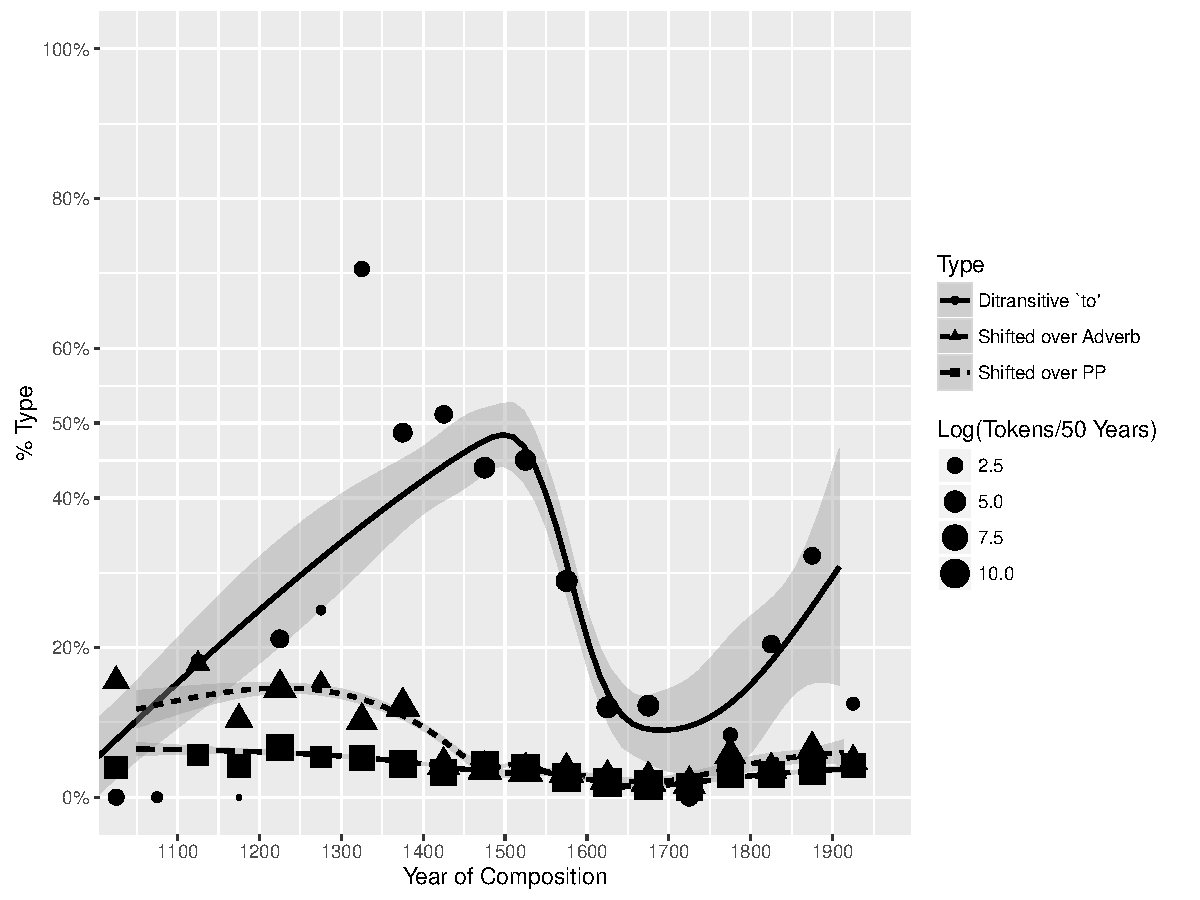
\includegraphics[width=\linewidth]{output/images/shifting}
	\caption{GAM smooth over weights of \textit{to} use in RT ditransitives and heavy NP shift over adverbs and PPs with noun phrase objects}
	\label{fig:shifting}
\end{figure}

Also, Figure \ref{fig:shifting} shows the rates of \textit{to} with RT ditransitives as well as the rates of heavy NP shift as estimated by the proportion of objects post-posed after adverbs and PPs with full noun phrase objects. Between 1450 and 1650, the rate of \textit{to} use is significantly different from the rate of heavy NP-shift (see Table \ref{tab:model-comp-heavy}). The significant difference in rates between \textit{to} in RT ditransitives and other post-posing operations in this time period indicates that these constructions are almost certainly \textbf{not} derived via post-posing the theme from a TR construction.

In other words, up until about 1400, \textit{to} was being used to mark recipients in all syntactic positions, which supports the notion that recipients are base generated as PPs independently of the surface word order. In chapter \ref{ch:diachron}, I show how quantitative tools from the study of diachronic syntax are able to tease apart the initial spread of \textit{to} from the subsequent development of the allomorphy grammar. The details of the statistics can be found there, but the conclusion is that there is evidence that \textit{to} initially spread through all environments at the same rate and that a subsequent change affected the RT orders (the development of the dative shift grammar).

\section{Syntax of Recipients}\label{sec:synrecp}
The previous sections argued that recipients and goals occur in distinct syntactic constructions and that the difference between dative case and prepositions is a purely surface morphological alternation. In this section, I propose a analysis for the syntactic positions for goals and recipients. As hinted at above, I follow the rest of the literature (e.g., \citet{Jackendoff.1990,Harley.2002,Hallman.2015}) in analysing goals as being introduced in a prepositional object construction (i.e., as the object of V). For the recipient, I follow \cite{McGinnis.1998,Bruening.2010,Bruening.2010b} in assuming that the recipient is introduced in an applicative head above the VP as discussed in the previous chapter. Theme--recipient word orders are derived by scrambling the theme into a second specifier of the applicative phrase (a view first suggested for English in \citet{Takano.1998}). In the following section, I show the following: the theme can marginally reconstruct from its scrambled position (using tests for asymmetric c-command), typological evidence that the RT order is base generated and the TR order is derived, and High German specific evidence that the derivation operation is scrambling. I then further support the transformational account for English by responding to criticisms of such accounts from the literature. Finally, I use data from Low German to support the idea that scrambling occurs even in morphologically poor languages (c.f. \citealt{Weerman.1997}). 
	\subsection{Asymmetric C-command}
	Binding asymmetries provide some of the clearest evidence for the internal structure of English ditransitive clauses. \cite{Barss.1986} showed that, in the RT order, the recipient systematically asymmetrically c-commands the theme. \cite{Aoun.1989} showed that, in the TR order, the theme systematically asymmetrically c-commands the recipient.  Anaphor Binding (\ref{ex:en-anaphor}), Superiority (\ref{ex:en-superiority}) and Negative Polarity (\ref{ex:en-negpol}) all show the surface c-command possibilities, in which the leftmost element asymmetrically c-commands the rightmost element (examples adapted from \cite{Aoun.1989}).
\begin{exe}
	\ex English, Anaphor Binding:\label{ex:en-anaphor}
\begin{xlist}
\ex Recipient--theme: I showed Mary herself (in the mirror).
\ex Recipient--theme: *I showed herself Mary (in the mirror).
\ex Theme--recipient: I showed Mary to herself (in the mirror).
\ex Theme--recipient: *I showed herself to Mary (in the mirror).
\end{xlist}
\ex English, Superiority:\label{ex:en-superiority}
\begin{xlist}
\ex Recipient--theme: Who did you give which check?
\ex Recipient--theme: *Which paycheck did you give who?
\ex Theme--recipient: Which check did you give to who?
\ex Theme--recipient: *Who did you give which check to?
\end{xlist}
\ex English, Negative Polarity:\label{ex:en-negpol}
\begin{xlist}
\ex Recipient--theme: I showed no one anything.
\ex Recipient--theme: *I showed anyone nothing.
\ex Theme--recipient: I showed nothing to any one.
\ex Theme--recipient: *I showed anything to no one.
\end{xlist}
\end{exe}

However, when looking at binding tests that allow for reconstruction (quantifier binding and each...the other), the recipient binding the theme is (marginally) possible in the TR order. In the RT order, the binding relationship is completely fixed. 

\begin{exe}
	\ex English, Quantifier Binding:\label{ex:en-qb}
\begin{xlist}
\ex Recipient--theme: I gave every worker$_i$'s mother his$_i$ paycheck.
\ex Recipient--theme: * I gave his$_i$ mother every worker$_i$'s paycheck.
\ex Theme--recipient: I gave every worker$_i$'s paycheck to his$_i$ mother.
\ex Theme--recipient: ? I gave his paycheck to every worker$_i$'s mother.
\end{xlist}

\ex English, Each...the other:\label{ex:en-eachother}
\begin{xlist}
\ex Recipient--theme: I showed each man the other's friend.
\ex Recipient--theme: * I showed the other's friend each man.
\ex Theme--recipient: I showed each man to the other's friend.
\ex Theme--recipient: ? I showed the other's friend to each man.
\end{xlist}
\end{exe}

German shows a similar pattern to the English data discussed above with a bias towards surface scope, such that a quantifier needs to c-command any bound pronouns on the surface. This can be seen in the RT order, where there is no availability of reconstruction (since no movement has taken place).

\begin{exe}
	\ex High German, RT:\label{ex:hg-binding-rt}
\begin{xlist}
\ex[ ]{\gll dass Maria jedem seinen Nachbarn vorgestellt hat.\\
that Maria everyone.DAT his.ACC neighbour.ACC introduced has.\\
\trans `that Maria introduced everyone his neighbor \citep[ex. 11a]{Lee.1994}.'}
\ex[*]{\gll dass Maria seinem Nachbarn jeden vorgestellt hat.\\
	that Maria his.DAT neighbour.DAT everyone.ACC introduced had.\\
	\trans `that Maria introduced everyone to his neighbour \citep[ex. 9a]{Lee.1994}.'}
\end{xlist}
\end{exe}

In the TR order, the theme can easily scope over/bind into the recipient. However, the recipient is also able to marginally scope over/bind into the theme. The judgements here are subject to speaker variation, but there are some speakers who allow the scrambled theme to reconstruct (for example to prevent a weak crossover violation). This is consistent with the idea that the theme has moved from a position under the recipient and can (marginally) reconstruct to that position at LF.

\begin{exe}
	\ex High German, TR:\label{ex:hg-binding-tr}
\begin{xlist}
	\ex[ ]{\gll dass Maria jeden seinem Nachbarn vorgestellt hat.\\
	that Maria everyone.ACC his.DAT neighbour.DAT introduced had.\\
	\trans `that Maria introduced everyone to his neighbour \citep[ex. 10a]{Lee.1994}.'}
	\ex[\%]{\gll dass Maria seinen Nachbarn jedem vorgestellt hat.\\
	that Maria his.ACC neighbour.ACC everyone.DAT introduced had.\\
	\trans `that Maria introduced everyone his neighbour \citep[ex. 12a (note 10)]{Lee.1994}.'}
\end{xlist}
\end{exe}

Taken together the binding/scoping facts in English and German suggest that the recipient is based generated higher than the theme. The marginal ability for the theme to be bound by/scope under the recipient in TR word orders suggests that the TR word order is derived by moving the theme above the recipient. The theme is thus typically interpreted as c-commanding the recipient, but can marginally reconstruct to its base position, where the recipient c-commands the theme. Since there is no movement in the base generated RT order, no reconstruction is possible and the recipient has to asymmetrically c-command the theme \citep{Takano.1998}.

	\subsection{Evidence for scrambling}
	I start this section on scrambling by presenting typological evidence in support of the notion that the RT order is basic and the TR order is derived. The basic order should be available in all languages, and indeed the RT order is available in all Germanic languages:
	\begin{exe}
\ex
\begin{xlist}
	\ex Icelandic: \label{ex:ice-rt}
\gll P\'{e}tur gaf konunginum amb\'{a}ttina.\\
Peter.NOM gave king.DEF.DAT maid-servant.DEF.ACC.\\
\trans `Peter gave the king the maid-servant.'
\ex Faroese:\label{ex:far-rt}
\gll Hon gav Mariu troyggiuna.\\
She gave Maria.DAT sweater.DEF.ACC.\\
\trans `She gave Maria the sweater \citep{Lundquist.2013b}.'
\ex Standard Norwegian: \label{ex:nor-rt}
\gll Jeg har gitt mannen boken.\\
I have given man.DEF book.DEF.\\
\trans `I gave the man the book \citep[ex 10]{Sprouse.1995}.'
\ex Swedish:\label{ex:sw-rt}
\gll Jag gav Johan en bok.\\
I gave John a book.\\
\trans `I gave John a book \citep{Holmberg.1995}.'
\ex Danish:\label{ex:dan-rt}
\gll Peter viste jo Marie bogen.\\
Peter showed indeed Mary book.DEF.\\
\trans `Peter indeed showed Mary the book \citep{Vikner.1989}.'
\ex High German:\label{ex:hg-rt}
\gll weil er der Unehrlichkeit keine Chance gibt.\\
as he.NOM the.DAT dishonesty no.ACC opportunity gives.\\
\trans `as he gives dishonesty no opportunity \citep[162]{Draye.1996}.'
\ex Yiddish:\label{ex:yid-rt}
\gll Zi git der snjjer dus pékl. \\
she.NOM gives the.DAT daughter-in-law the.ACC parcel.\\
\trans 'She gives her daughter-in-law the parcel \citep[ex 190a]{Birnbaum.1979}.'
\ex Dutch:\label{ex:dut-rt}
\gll Ik heb (aan) Jan een boek gegeven.\\
I have (to) Jan a book given.\\
\trans `I gave Jan a book \citep{Tiersma.1985}.'
\ex Afrikaans:\label{ex:af-rt}
\gll dat die man die vrou `n dokument gegee het.\\
that the man the woman a document given has.\\
\trans `...that the man gave a document to the woman \citep{Louw.2012}.'
\ex Frisian:\label{ex:fri-rt}
\gll se joech jar kammeraatske in skjirre.\\
she gave her girlfriend a {pair of scissors}.\\
\trans `She gave her girlfriend a pair of scissors.'
\ex Low German: \label{ex:lg-rt}
\gll ick gaw den Mann dat Brod.\\
I gave the man the bread.\\
\trans `I gave the man the bread \citep{Mussaus.1829}.'
\ex English: I gave the man the book.\label{ex:eng-rt}
\end{xlist}
\end{exe}

Most of the Germanic languages\footnote{I do not have data on the availability of TR orders in Yiddish. See below for Icelandic} also allow TR word orders (as discussed above the difference between prepositions and dative case is syntactically irrelevant).

\begin{exe}
	\ex \label{ex:preprec}
	\begin{xlist}
		\ex[\%]{Faroese\footnote{Faroese is currently undergoing a change, where dative shift is becoming a regular part of the language. The \% indicates the variation seen between people, who have adopted this change versus those who have not. For those who have not adopted this change, Faroese behaves like Icelandic, which is described below.}:\label{ex:far-tr}
		\gll Hon gav telduna til gentuna.\\
		she gave computer-the.ACC to girl-the.ACC\\
		\trans `She gave the computer to the girl.'}
		\ex Norwegian:\label{ex:nor-tr}
		\gll Vi har lånt den interessante boken du nevnte *(til) Petter.\\
		we have lent the interesting book you mentioned to Peter.\\
		\trans `We have lent the interesting book you mentioned to Peter \citep{Larson.1988}.'
		\ex Swedish:\label{ex:sw-tr}
		\gll Jag gav en bok *(til) Johan.\\
		I gave a book to John.\\
		\trans `I gave a book to John \citep{Holmberg.1995}.'
		\ex Danish:\label{ex:dan-tr}
		\gll Jeg gav bogen *(til) Anna.\\
		I gave book.the to Anna.\\
		\trans `I gave the book to Anna\citep{Holmberg.1998}.'
		\ex High German:\label{ex:hg-tr}
		\gll weil er keine Chance der Unehrlichkeit gibt.\\
		as he.NOM no.ACC opportunity the.DAT dishonesty gives.\\
		\trans `as he gives no opportunity to dishonesty'
		\ex Dutch:\label{ex:dut-tr}
		\gll Ik heb een boek *(aan) Jan gegeven.\\
		I have a book *(to) Jan given.\\
		\trans `I gave a book to Jan.'
		\ex Afrikaans:\label{ex:af-tr}
		\gll Ek het `n fooitjie aan hom gegee.\\
		I have a tip to him given.\\
		\trans `I have given a tip to him \citep{Stadler.1996}.'
		\ex Frisian:\label{ex:fri-tr}
		\gll ik joech in plant oan Beppe.\\
		I gave a plant to Grandmother.\\
		\trans `I gave a plant to Grandmother \citep{Tiersma.1985}.'
		\ex Low German:\label{ex:lg-tr}
		\gll ick gaw dat Brod den Man, wobei dat Brod zeigend ist.\\
		I gave the bread the man who the bread shown is.\\
		\trans `I gave the bread to the man who was shown the bread \citep{Mussaus.1829}.'
		\ex English: I gave the book to the man.\label{ex:en-tr}
	\end{xlist}
\end{exe}

	However, Modern Icelandic does not allow TR orders except as the product of heavy NP shift \citep{Dehe.2004}.

\begin{exe}
	\ex Icelandic:\label{ex:ice-tr}
\gll ?*Hann gaf amb\'attina konunginum.\\
He.NOM gave maid-servant.DEF.ACC king.DEF.DAT. \\
\trans `He gave the king the maid-servant \citep[ex 14b]{Dehe.2004}.'
\end{exe}

The universality of the RT order and the unavailability of TR orders in some languages suggest that the RT order is basic and the TR order derived (with Modern Icelandic lacking the TR deriving transformation). \cite{Georgala.2011} provides evidence from stranded depictives, floating quantifiers and split topics that all support the notion that the RT order is basic in High German. High German also provides additional evidence that the transformation under discussion is scrambling \citep{Lenerz.1977,Abraham.1986,Webelhuth.1992,Choi.1996}.

\cite{Lenerz.1977} showed that all scrambling in High German is sensitive to information focus (i.e. the focus received by new information), but not contrastive focus. In particular, words that receive new information focus cannot be targeted by scrambling operations. \cite{Lenerz.1977} applied this heuristic to ditransitives and discovered that recipient ditransitives had the following pattern. When recipients received information focus (e.g., by being the answer to a wh-question), both RT and TR word orders were possible. This would be consistent with either of the following analyses: the two word orders are not derived via scrambling or the recipient is not the element that scrambles.

\begin{exe}
	\ex High German, Recipient Focus \citep{Choi.1996}:\label{ex:hg-rec-focus}
\gll Wem hast du das Geld gegeben?\\
whom.DAT have you.NOM the money.ACC given\\
\trans `Who did you give the money to?'
\begin{xlist}
\ex \gll Ich habe dem KASSIERER das Geld gegeben.\\
I.NOM have the cashier.DAT the money.ACC given.\\
\trans `I have given the cashier the money.'
\ex \gll Ich habe das Geld dem KASSIERER gegeben.\\
I.NOM have the money.ACC the cashier.DAT given.\\
\trans `I have given the money to the cashier.'
\end{xlist}
\end{exe}

However, when the theme receives information focus, only the RT word order is possible. Given the constraints on scrambling in High German, this indicates that the RT order is base generated and that the TR order is derived via scrambling the theme above the recipient.

\begin{exe}
	\ex High German, Theme Focus \citep{Choi.1996}:\label{ex:hg-theme-focus}
	\gll Was hast du dem Kassierer gegeben?\\
what.ACC have you.NOM the cashier.DAT given\\
\trans `What did you give to the cashier?'

\begin{xlist}
	\ex[ ]{\gll Ich habe dem Kassierer das GELD gegeben.\\
I.NOM have the cashier.DAT the money.ACC given.\\
\trans `I have given the cashier the money.'}
\ex[?*]{\gll Ich habe das GELD dem Kassierer gegeben.\\
I.NOM have the money.ACC the cashier.DAT given.\\
\trans `I have given the money to the cashier.'}

\end{xlist}
\end{exe}

In Example (\ref{ex:german-VP-top}), repeated below, I presented evidence from VP-fronting that the scrambling occurs within the verb phrase. This conclusion can be drawn from the fact that both word orders are grammatical inside of a fronted VP. Since High German is a V2 language, only one phrase is able to occur before the finite verb. In this case, the phrase is the VP and thus all material inside the fronted element must be inside of the verb phrase (i.e., not part of the T domain).

	\begin{exe}
		\exr{ex:german-VP-top} High German, VP-topicalisation:
		\begin{xlist}
			\ex \gll  Dem Mann das Buch gegeben habe ich, (nicht der Frau dEN Film geschenkt).\\
			the.DAT man the.ACC book given have I, (not the.DAT woman the.ACC film sent).\\
			\trans `It was giving the man the book that I did (not sending the woman the film).'
			\ex \gll Das Buch dem Mann gegeben habe ich, (nicht dEN Film der Frau geschenkt).\\
			the.ACC book the.DAT man given have I, (not the.ACC film the.DAT woman sent).\\
			\trans `It was giving the book to the man that I did (not sending the film to the woman).\\
		\end{xlist}
	\end{exe}

Another piece of evidence is that both word orders can occur after vP-level adverbs (such as negation). In combination, these facts show that the site of the scrambling is within the verb phrase (i.e., no higher than Voice).

\begin{exe}
	\ex High German, VP-level adverbs:\label{ex:hg-VPadverb}
	\begin{xlist}
		\ex \gll Ich habe nicht dem Mann das Buch gegeben, SONDERN DER FRAU DEN FILM GESCHENKT.\\
		I have not the.DAT man the.ACC book given, but the.DAT woman the.ACC film sent.\\
		\trans `I didn't give the man the book, instead I sent the woman the film.'
		\ex \gll Ich habe nicht das Buch dem Mann gegeben, SONDERN DEN FILM DER FRAU GESCHENKT.\\
		I have not the.ACC book the.DAT man given, but the.ACC film the.DAT woman sent.\\
		\trans `I didn't give the book to the man, insead I sent the film to the woman.'
	\end{xlist}
\end{exe}

This subsection showed that High German provides solid language internal evidence that TR word orders are derived via scrambling from RT orders. This scrambling targets a position within the verb phrase. Since the operation is necessary to account for the High German data, the most parsimonious account of TR orders in other languages would use the same operation.

\subsection{Replies to Arguments Against Transformational Analysis of English Dative Shift}

Since \cite{Oehrle.1976}, there has been an argument that English dative shift should not receive a transformational analysis, because there are interpretive differences between the RT and TR constructions. One of the interpretive differences is the existence of a completion implicature in the RT order.

\begin{exe}
	\ex Modern English:\label{ex:en-implicature}
	\begin{xlist}
		\ex[\#]{John taught the students French, but they didn't learn French}
		\ex[ ]{John taught French to the students, but they didn't learn French}
	\end{xlist}
\end{exe}

\cite{Hovav.2008} show that this completion implicature is actually the product of individual verbs and not directly attributable to the order of the objects. For example, \textit{give} entails successful transfer no matter which order the objects are in, and \textit{offer} does not entail it in either variant (it entails successful transfer in all plausible worlds in which the offer if accepted).

\begin{exe}
	\ex English, `give', \citep[exx 36 \& 37]{Hovav.2008}:\label{ex:en-implicature-give}
	\begin{xlist}
		\ex[\#]{My aunt gave my brother some money for new skis, but he never got it}
		\ex[\#]{My aunt gave some money to my brother for new skis, but he never got it}
	\end{xlist}
	\ex English, `offer', \citep[exx 38 \& 39]{Hovav.2008}:\label{ex:en-implicature-offer}
	\begin{xlist}
		\ex Max offered the victims help, but they refused his offer.
		\ex Max offered help to the victims, but they refused his offer.
	\end{xlist}
\end{exe}

\cite{Oehrle.1976}, also, demonstrated that there were a number of different type of recipient interpretations associated even with verbs like GIVE. He argued that one of the interpretations was only available in the RT order. This interpretation involves abstract possession. The classic example is given below:

\begin{exe}
	\ex English: Nixon gave Mahler a book.\label{ex:en-nixon-rt}
	\begin{xlist}
		\ex[ ]{Nixon gave Mahler a physical object (namely a book)}
		\ex[ ]{Nixon gave Mahler an idea (that Mahler wrote into a book)}
	\end{xlist}
	\ex English: Nixon gave a book to Mahler.\label{ex:en-nixon-tr}
	\begin{xlist}
		\ex[ ]{Nixon gave Mahler a physical object (namely a book)}
		\ex[*]{Nixon gave Mahler an idea (that Mahler wrote into a book)}
	\end{xlist}
\end{exe}

These abstract interpretations inevitably involve coercing the verb into a verb of creation, since the abstract entity always comes into being by the act of giving. \cite{Frey.2001} shows that in German indefinite objects under verbs of creation have to remain in base position (i.e. they must occur to the right of manner adverbs).

\begin{exe}
	\ex High German \citep[ex 31]{Frey.2001}:\label{ex:hg-creation}
	\begin{xlist}
		\ex[ ]{\gll dass Hans geschickt eine Flöte schnitzte\\
		that John skillfully a.ACC flute carved\\
	\trans `that John skillfully carved a flute.'}
	\ex[*]{\gll dass Hans eine Flöte geschickt schnitzte\\
		that John a.ACC flute skillfully carved\\
	\trans `that John skillfully carve a flute.'}
	\end{xlist}
\end{exe}

The fact that the objects cannot scramble in German, in combination with the German predilection for surface interpretation \citep{Beck.1996}, supports the conclusion that at LF these objects need to be in their base position. That the object of verbs of creation must be interpreted in its base position explains why \textit{to} variants are generally prohibited when verbs of transfer are coerced into a creation interpretation (when the theme comes into being as part of the transfer), which \cite{Bruening.2010b} used as an argument against a transformational account of dative shift in English.

\begin{exe}
	\ex English \citep[ex. 2]{Bruening.2010b}:\label{ex:en-creation}
	\begin{xlist}
	\ex[ ]{The lighting here gives me a headache}
	\ex[*]{The lighting here gives a headache to me}
	\end{xlist}
\end{exe}

The same interpretive pressure exists in cases of idioms. Under the assumption that at LF idiomatic objects need to form a constituent with the verb in order to receive an idiomatic interpretation, scrambled idiomatic objects would need to obligatorily reconstruct promoting the RT order. Under the assumption that reconstruction is costly, there must be some countervailing pressure that would motivate the scrambling (see \citep{Bruening.2010,Bruening.2010b,Bruening.2014} for a discussion of possible motivating pressures).

\begin{exe}
	\ex English \citep[ex 3]{Bruening.2010b}:\label{ex:en-idioms}
	\begin{xlist}
		\ex[ ]{The count gives me the creeps}
		\ex[*]{The count gives the creeps to me}
	\end{xlist}
\end{exe}

The scrambling analysis is also able to more easily explain some of the purpose clause facts from \citet{Hallman.2015}. Hallman suggests that the TR order is derived via internal passivisation from the RT order (see \citet{Larson.1988}). However, he notes that this gets the standard word order between the recipient and purpose clause wrong (\ref{ex:recipient--purpose}), since the recipient would be a right adjoined adjunct in a higher phrase than the purpose clause. He is thus forced to argue that the purpose clause obligatorily scrambles above the recipient adjunct (see (\ref{ex:hallman-tree})).

\begin{exe}
	\ex \label{ex:recipient--purpose} English \citep[ex 25]{Hallman.2015}:\label{ex:en-purpose-order}
	\begin{xlist}
		\ex[*]{Mary gave a puppy to play with to John}
		\ex[ ]{Mary gave a puppy to John to play with}
	\end{xlist}
\end{exe}

In (\ref{ex:comparison-trees}), I show trees of both the scrambling analysis (following the scrambling structure provided in \cite{McGinnis.1998}) pursued here and Hallman's analysis. In both cases, the recipient scopes over the purpose clause (unlike with goals, where the goal PP scopes under the purpose clause). Under the scrambling analysis, the word order falls out without any alterations, since the recipient is still in the left attached specifier of the applicative phrase.

\begin{exe}
\ex \label{ex:comparison-trees}
\begin{xlist}
\ex Scrambling Analysis: \\
\xymatrix@=1pt{
 & vP\ar@{-}[dl]\ar@{-}[dr]\\
DP\ar@{-}[d] & & \bar{v}\ar@{-}[dl]\ar@{-}[dr]\\
\text{Mary} & \text{v} & & ApplP\ar@{-}[dl]\ar@{-}[dr]\\
 & & DP\ar@{-}[d] & & \bar{Appl}\ar@{-}[dl]\ar@{-}[dr]\\
 & & \text{the book$_{i}$}\ar@{<-}@(dl,dl)[ddrrr] & DP\ar@{-}[d] & & \bar{Appl}\ar@{-}[dl]\ar@{-}[dr]\\
 & & & \text{to John} & Appl & & VP\ar@{-}[dl]\ar@{-}[dr]\\
 & & & & & DP_{i} & & \bar{V}\ar@{-}[dl]\ar@{-}[dr]\\
 & & & & & & V\ar@{-}[d] & & CP\\
 & & & & & & \text{give}& & \text{Op$_{k}$ PRO$_{i}$ to play with t$_{k}$}}
 \ex\label{ex:hallman-tree} Hallman's Analysis: \\
 \xymatrix@=1pt{&vP_{1}\ar@{-}[dl]\ar@{-}[dr]\\
DP\ar@{-}[d] && \bar{v_{1}}\ar@{-}[dl]\ar@{-}[dr]\\
\text{Mary}&v_{1}\ar@{-}[d]&&vP_{2}\ar@{-}[dl]\ar@{-}[dr]\\
&CAUSE&\Delta&&\bar{v_{2}}\ar@{-}[dl]\ar@{-}[dr]\\
&&&\bar{v_{2}}\ar@{-}[dl]\ar@{-}[dr]&&PP\ar@{-}[d]\\
&&v_{2}&&VP\ar@{-}[dl]\ar@{-}[dr]&\text{to John}\\
&&&DP\ar@{-}[d]&&\bar{V}\ar@{-}[dl]\ar@{-}[dr]\\
&&&\text{a picture}&V\ar@{-}[d]&&CP\ar@{-}[d]\\
&&&&\text{HAVE}&&\text{Op$_{k}$ PRO$_{i}$ to play with t$_{k}$}\\}
\\
\end{xlist}
\end{exe}%13 - Tree with V' attached purpose clause

A potential problem for the scrambling analysis in English is the existence of verbs that only occur in the TR order (verbs that only occur in the RT order can be explained as lacking the scrambling operation). These verbs (e.g., DONATE) form an ill defined class that shows a great deal of inter-speaker variation \citep{Levin.1993}. I propose that there is also interspeaker variation in the orgin of the unacceptability judgements for these verbs. For some speakers, it is plausible that these verbs are analysed as introducing goals instead of recipients. In this case, the \textit{to}-marked elements are the complement of the main verb and thus the TR order arises by default. The availabilty of goal thematic roles in Icelandic in the same situation (i.e., cases of donation) suggests that this reanalysis is plausible.

\begin{exe}
	\exr{ex:icelandic-goals} Icelandic:
	\gll \'{E}g gaf b\ae kurnar til H\'ask\'olab\'okasafnsins\\
	I.NOM gave books.the.ACC to University.Library.the.GEN\\
	\trans `I gave the books to the University Library'
\end{exe}

However, \cite{Hallman.2015} presents his judgements that suggest that even the object of these verbs are in the specifier of an applicative (namely that for him, their recipient objects are able to bind into purpose clauses). To the extent that these sentences are acceptable, the goal reanalysis is untenable.

\begin{exe}
	\ex English (ex. 48 from \citealt{Hallman.2015}):\label{ex:en-purpose-donate}
	\begin{xlist}
		\ex John donate money$_{j}$ to the church$_{i}$ [PRO$_{i}$ to buy candles with e$_{j}$].
		\ex Mary submitted a draft$_{j}$ to the professor$_{i}$ [PRO$_{i}$ to comment on e$_{j}$].
		\ex Mary returned the books$_{j}$ to John$_{i}$ [PRO$_{i}$ to reshelve e$_{j}$].
		\ex John revealed the plan$_{j}$ to Mary$_{i}$ [PRO$_{i}$ to consider e$_{j}$].
		\ex Mary demonstrated the technique$_{j}$ to John$_{i}$ [PRO$_{i}$ to teach e$_{j}$ to the new assistants].
	\end{xlist}
\end{exe}

However, a similar problem arises when looking at the behaviour of recipients in Romance languages (esp. since the English verbs are often characterised as being predominantly borrowed from Romance). The typical word order for recipients in Romance languages is TR and the recipient is obligatorily marked with a preposition (unless it has cliticised to the verb, where prepositional marking is prohibited).

\begin{exe}
\ex Italian \citep[sec. 4.3.1]{Proudfoot.2013}
\begin{xlist}
\ex \gll Ho dato il libro *(a) Paolo.\\
I.NOM gave the book to Paolo.\\
\trans `I gave the book to Paolo.'
\ex \gll Ho dato il libro *(a) LUI.\\
I.NOM gave the book to him.\\
\trans `I gave the book to HIM.'
\ex \gll (*A) gli ho dato il libro.\\
to him.DAT I.NOM gave the book.\\
\trans `I gave him the book.'
\end{xlist}
\end{exe}%22 - French examples

If the TR order is the only one that occurs, that would seem to be a refutation of the universaility of a RT base generation order, especially since requiring scrambling seems unsatisfactory. However, while TR orders are (vastly) preferred in Romance languages, there exists evidence that they are derived via the same VP-internal scrambling operation as in Germanic languages. In particular, Italian shows the same sensitivity to informaiton focus described for German, suggesting that just as in German, the TR order is derived from the RT order via scrambling.

\begin{exe}
\ex Italian \citep[ex 26]{Belletti.1995}:
\gll Che cosa hai restituto a Maria?\\
what did you.NOM {give back} to Maria?\\
\trans `What did you give back to Maria'
\begin{xlist}
\ex[ ]{\gll Ho restituto a Maria le chiavi.\\
I.NOM {give back} to Maria the keys\\
\trans `I gave back the keys to Maria'}
\ex[*]{\gll Ho restituto le chiavi a Maria.\\
I.NOM {give back} the keys to Maria\\
\trans `I gave back the keys to Maria'}
\end{xlist} 
\end{exe}%23 - Italian A-scrambling

Even though the Romance TR order is derived from VP-internal scrambling, it is necessary to explain why the operation is as restricted as it is in Romance, given that it applies much more freely in Germanic languages. At this point, it becomes useful to return to the distinction between grammar and use discussed in Chapter 1. A grammar generates the possible utterances of the language (i.e., it creates a possibility space). However, not all grammatical possibilities are equally natural (e.g., ``the button machine with letters'' is a perfectly grammatical way of referring to a ``keyboard'', but is not the way any native speaker of English would avail themselves of). Speakers of a language conform as a community on determining how the possibilities of their grammar will be deployed in order to satisfy various demands (including information structure, prosodic naturalness, social signalling, among others). The difference between Germanic and Romance can be attributed to the way in which the possibilities generated by the scrambling grammar are deployed in actual language use.

As discussed in Chapter \ref{ch:introduction}, unacceptability can, but need not, be derived from ungrammaticality. Corpus studies of dative shift \citep{Collins.1995,Bresnan.2007,Bresnan.2009} have shown that even when all other factors are kept constant (e.g., length of objects, information status of objects, etc.), there is a great deal of between verb variation in the probability of the RT and TR word orders. \cite{Bresnan.2010} use a series of gradient acceptability judgement tasks to show that degree of acceptability of a particular word order is strongly predicted by its corpus frequency (i.e., the more likely a particular sentence is to occur in the RT order in a corpus, the more acceptable participants tended to rate it). This suggests that one source of unacceptability is an extra--grammatical dispreference for the use of certain grammatical constructions (i.e., just because a grammar generates a sentence does not mean that any native speaker of the language would use that sentence or that it will sound natural). 

By associating the DONATE class's TR preference to the independently necessary verb specific patterns of use, the grammar of recipient ditransitives can be kept simple and universal. The verb specific nature, also, explains why there is so much inter-speaker variation as to which verbs belong in the DONATE class. Each speaker needs to estimate the probability of scrambling and not-scrambling for each verb; some speakers assign such a strong lexical probability to scrambling that no other factors can override it, while other speakers assign a weaker lexical probability to the same verb moving it out of the class. The tendency for verbs of similar types to pattern together (see \citealt{Levin.1993}) can be explained by the need for speakers to often estimate lexical probability from extremely small number of attestations of a particular lexical item in their input. In those situations, a sensible strategy is to group a number of phonologically/semantically related verbs together and estimate the lexical probability of each individual verb on the basis of the group corpus.

Some evidence that DONATE does not categorically prohibit RT orders, but simply strongly disprefers them, comes from cases in which all of the other contextual factors conspire to support the RT order. This situation arises in cases of organ donation, where the recipient of the donation is animate and can be realised pronominally. In this case, (\ref{ex:kidney}) are generally judged more acceptable than (\ref{ex:donate-inanim}). Indeed, a Google search for ``donated him a kidney'' had 71 hits, suggesting that a number of English speakers find the construction grammatical.

\begin{exe}
	\ex Modern English:\label{ex:en-donate}
	\begin{xlist}
		\ex[*]{John donated him a kidney.}\label{ex:kidney}
		\ex[?]{John donated the library books.}\label{ex:donate-inanim}
	\end{xlist}
\end{exe}

Over the last forty years, scholars have brought a number of arguments against transformational accounts of English RT and TR word orders. Many of the accounts rely on the confusion between goals and recipients. In the case of idioms and abstract interpretations of themes, the scrambling account provides an explanation for why the RT order is preferred based on restrictions on interpretation of themes and the objects of verbs of creation. Finally, two possible explanations for the inability of verbs like DONATE to occur in the RT word order. One explanation claimed that speakers had reanalysed the indirect object of these verbs as goals. The other explanation relied on extra-grammatical variation in the probability of using the TR and RT orders based on individual verbs. The purpose of this section is to maintain the possibility of a transformational account of English ditransitive word orders and thus licensing the VP-internal scrambling analysis of TR orders in English.

\subsection{Scrambling and Overt Marking}

While scrambling has been considered a standard operation in morphologically rich languages, it has been considered rare (or impossible) in languages without overt case marking (see for example \citealt{Weerman.1997}). However, Low German provides an example of a language that lacks case marking, but maintains scrambling syntax. For example, \cite{Fleischer.2006} states: ``In Low German, this construction [prepositional dative marking] could eventually be viewed as compensatory to the loss of a distinct dative case; however, from the fact that I could not find any decisive examples of this construction in Low German, I conclude that it is very rare.'' \cite{Lindow.1998} makes no mention of prepositional dative marking (including in a section discussing the uses of various prepositions). Indeed, \cite{Mussaus.1829} gives examples of TR clauses without any prepositional marking, even though the dative/accusative distinction had been lost hundreds of years before Mussäus wrote his grammar \citep{Lasch.1914,Boden.1993}.

\begin{exe}
	\exr{ex:lg-tr} Low German:
	\gll ick gaw dat Brod den Man, wobei dat Brod zeigend ist.\\
	I gave the bread the man who the bread shown is.\\
	\trans `I gave the bread to the man who was shown the bread \citep{Mussaus.1829}.'
\end{exe}

The opposite counterexample also holds. Only one Germanic language clearly lacks scrambling (i.e., lacks TR word orders), namely Icelandic (see above). However, Icelandic still has a robust morphological case marking. When considered together, the data from Low German and Icelandic show that there is no intrinsic connection between robust case marking and scrambling. All possible combinations of weak/robust case marking and scrambling/no scrambling are attested.

\section{Conclusions}
In this chapter, I argued on the basis of data from active clauses that recipients are always introduced as a PP in the specifier of an applicative phrase, which means that RT word orders are always the base generated orders. Goals, on the other hand, are introduced as a PP object in the complement of the verb. The claimed universal nature of these syntactic orders supports a strong version of the Uniformity of Theta Assignment Hypothesis \citep{Baker.1988}, namely that all languages share the same base generation orders for the same theta roles.
	Typological evidence as well as language specific evidence from High German and English was brought to demonstrate that TR orders are derived from scrambling. All Germanic language have RT orders, but Icelandic lacks the TR order. High German internal evidence and data from marginal reconstruction in TR orders supports the notion that the theme is moving from a base position below the recipient to its surface position.
	The difference between dative case and prepositional marking was reduced to contextual allomorphy in the realisation of the dative P head. This morphological distinction was shown to sometimes correlate with the recipient/goal distinction, but was often independent. Evidence from Low German and Icelandic showed that the availability of scrambling is completely independent of the richness of surface morphology.

%\bibliography{diss}

%\part{Passive Ditransitives}\label{part:pas}
\chapter{Passive Syntax of Recipient Ditransitives}\label{ch:passive}
\section{Introduction}
This chapter analyses how data from the passivisation of recipient ditransitives can be explained by the dative PP + applicative analysis. Passivisation, as a movement operation, is a useful probe in studying the internal structure of clauses. As discussed in Chapter \ref{ch:theoryback}, the assignment of subject properties to arguments shows sensitivity to case and locality issues that reflect on the case and syntactic positions of arguments.

This chapter will start by analysing recipient passivisation. Since (as argued in Chapter \ref{ch:active}) the recipient always receives dative case, which is represented by a PP, full recipient passivisation (with a nominative recipient) requires dative--to--nominative conversion. Building on the analysis of \cite{Alexiadou.2014}, I propose that dative--to--nominative conversion involves incorporation of the P head into a verbal element, which turns the recipient into a bare DP and makes it available for structural case assignment. The dative PP analysis assumes that the difference between inherent/lexical case and structural case is the presence of the PP layer \citep{Bayer.2001}. Evidence for the incorporation analysis will be brought from recipient passives in German, Dutch and Swedish. In the next subsection, I discuss oblique subjects in Icelandic and Faroese and argue for the parameterisation of the validity of PP subjects.

The second section focuses on theme passivisation. I show that there are two mechanisms by which the locality constraint can be violated, namely: (a) restricting subject movement to DPs and allowing T to consider multiple arguments for subject movement and (b) moving either the theme or the recipient so that the theme is the highest argument in an A-position. The first mechanism is a consequence of the P-incorporation analysis for recipient passivisation. If P-incorporation is unavailable, then the recipient is not a valid target for nominative case assignment. If T requires nominative subjects, then only the theme would be a valid subject. I show that some languages allow T to consider multiple arguments and move the theme across the recipient from its base generated position. In other languages, only the highest argument can be considered and either the recipient or theme must move in order for theme passivisation to occur.

\section{Recipient Passivisation}
In this dissertation, recipient passivisation is defined as cases where the recipient is in the higher subject position (i.e., spec-TP). There are two sub-cases of this situation, which will be addressed in turn. The first (dative-to-nominative raising) is a case where the recipient receives nominative case and has all subject properties. The second (oblique subjects) is a case where the subject properties are split with the recipient occupying the higher subject position, but the theme receiving nominative case.

\subsection{Dative-to-Nominative Raising}

The dative PP + applicative analysis claims that all recipients are dative case marked. Therefore, any example of a nominative recipient is an example of dative-to-nominative conversion. As will be shown below, this property can be seen on the surface in a number of Germanic languages (namely Faroese, Halsa Norwegian, and High German). 

Faroese\footnote{Faroese is currently changing from having oblique subjects like Icelandic (discussed below) and having dative-to-nominative raising. The data presented below are from the speakers that have adopted the new grammar with dative-to-nominative raising (see \cite{Eyorsson.2012} for a discussion of this change and survey data attesting to the existence of this sub-population).} and Halsa Norwegian both show the availability of dative-to-nominative conversion, although they do not elucidate the mechanism by which dative-to-nominative conversion occurs. Both languages have a clear morphological distinction between dative and accusative case:

\begin{exe}
	\ex Faroese:\label{ex:far-case}
		\begin{xlist}
			\ex[ ]{\gll Teir góvu \textbf{gentuni} telduna \\
				they gave \textbf{girl-the.DAT} computer-the.ACC \\
			            \trans `They gave the girl the computer.'}
				    \ex[*]{\gll Teir góvu \textbf{gentuna} telduna \\
				they gave \textbf{girl-the.ACC} computer-the.ACC \\
			    \trans `They gave the girl the computer.'}
		\end{xlist}
		\ex Halsa Norwegian:\label{ex:halsa-case}
	\begin{xlist}
		\ex \gll Ho erta \textbf{katt\aa} \\
		she teased \textbf{cat.DEF.ACC} \\
			\trans `She teased the cat.'
			\ex \gll Ho ga \textbf{katt\aa} inn mat \\
			she gave \textbf{cat.DEF.DAT} food \\
			\trans `She gave the cat food.'
	\end{xlist}
\end{exe}

Both languages also allow the dative argument to surface as nominative in the passive. Oblique subjects (of ditransitive passives) are marginal/ungrammatical \citep{Eyorsson.2012}:

\begin{exe}
	\ex Faroese:\label{ex:far-pass}
	\begin{xlist}
		\ex[ ]{\gll Gentan bleiv givin telduna\\
			    girl-the.NOM was given.NOM computer-the.ACC\\
		    	    \trans `The girl was given the computer.'}
		\ex[??]{\gll Gentuni bleiv givin ein telda\\
			    girl-the.DAT was givn.NOM a.NOM computer.NOM\\
		    	    \trans `The girl was given the computer.'}
	\end{xlist}
	\ex Halsa Norwegian:\label{ex:halsa-pass}
	\begin{xlist}
		\ex[ ]{\gll Hainn vart gjevinn ei skei.\\
He.NOM was given a spoon\\
\trans `He was given a spoon.' \cite[ex 50c]{Eyorsson.2012}}
\ex[*]{\gll Hånnå vart gjevinn ei skei.\\
He.DAT was given a spoon\\
\trans `He was given a spoon.' \cite[ex 50c]{Eyorsson.2012}}
	\end{xlist}
\end{exe}

In order to explain how dative-to-nominative conversion occurs, a theory of nominative case assignment needs to be given. As discussed in Chapter \ref{ch:theoryback}, I argue that all arguments marked with non-structural case are actually PPs, and that all and only arguments marked with structural case are bare DPs. Therefore, in order for an element to receive nominative case, it must be a bare DP. While the theme in recipient ditransitives is a DP, the recipient is a PP and thus should be unavailable for nominative case assignment. For it to become available, the PP layer must be removed.

In Chapter \ref{ch:theoryback}, I introduced the operation of P-incorporation as a means of converting PPs into DPs. This operation unites dative-to-nominative conversion with theories of pseudopassivsation, where passivisation of the object of preposition required incorporation of the preposition into the verbal domain \citep{Herslund.1984}. This section argues that both pseudopassivisation and nominative recipient passivisation rely on the same underlying mechanism of P-incorporation, however, the structural/semantic differences between prepositional objects (complements of the main verb) and recipients (specifiers of an applicative phrase) mean that pseudopassivisation and nominative recipient passivisation need not co-occur in the same language (or that the reflex of P-incorporation need not be the same across the two constructions in the same language).

P-incorporation is a type of head excorporation, which must be distinct from standard head movement. P-incorporation moves the P-head from the specifier of the recipient -- itself in the specifier of the applicative phrase -- and adjoins it to the head of the nearest C-commanding phrase. As argued in the previous chapter, Swedish verbs with prefixes are derived via P-incorporation, since they do not license theme--recipient orders (\ref{ex:Swedish-complex-act}). After VP-internal scrambling, the theme would C-command the recipient and thus be the nearest C-commanding phrase, making the theme rather than the verb the target of P-incorporation. Since the verb \textit{erbjoda} `offer' is built from P-incorporation, if the dative P does not incorporate, the verb cannot be used (since it cannot be built).
	\begin{exe}
		\exr{ex:Swedish-complex-act} Swedish:
			\begin{xlist}
				\ex[ ]{\gll Han erbjöd Jan ett nytt jobb\\
				he.NOM offered John a new job\\
			\trans `He offered John a new job'}
				\ex[??]{\gll Han erbjöd ett nytt jobb til Jan\\
				he.NOM offered a new job to John\\
			\trans `He offered a new job to John'}
				\ex[*]{\gll Han erbjöd ett nytt jobb Jan\\
				he.NOM offered a new job John\\
			\trans `He offered a new job to John'}
			\end{xlist}
	\end{exe}

	After reviewing some more data, I show that the target site of P-incorporation also has implications for the structure of OV and VO clauses, since OV and VO languages show different reflexes of P-incorporation. Example \ref{ex:VO-Pincorp} shows how P-incorporation in VO clauses can lead to prefixed verbs as in Swedish.

\begin{exe}
	\ex P-incorporation (VO Word Order)\label{ex:VO-Pincorp}\\
			\xymatrix@=2pt{
			& VoiceP\ar@{-}[dl]\ar@{-}[dr]\\
			V+Appl+Voice\ar@{<-}[dd] && ApplP\ar@{-}[dl]\ar@{-}[drr]\\
			& PP_{\text{Recipient}}\ar@{-}[dl]\ar@{-}[dr] & & & \bar{Appl}\ar@{-}[dl]\ar@{-}[dr]\\
			\text{\sout{P}} & & DP_{\text{Recipient}} & \text{\sout{Appl}} & & VP\ar@{-}[dl]\ar@{-}[dr]\\
			&  &  &  & \text{\sout{V}} & & DP_{\text{Theme}}}
\end{exe}


Dutch and High German show how OV languages show different surface properties. Recipient passivisation is not normally available in Dutch or High German, instead the theme must receive nominative case (see below for further discussion of theme passivisation).

\begin{exe}
	\ex High German:\label{ex:hg-normal-pass}
\begin{xlist}
	\ex[ ]{\gll Ich glaube, dass \textbf{den} \textbf{Kindern} das Fahrrad geschenkt worden ist.\\
	I beleive that \textbf{the.DAT.PL} \textbf{children} the.NOM bicycle given become be.3sg\\
\trans `I believe that the children were given the bicycle.'}
\ex[*]{\gll Ich glaube, dass \textbf{die} \textbf{Kindern} das Fahrrad geschenkt worden sind.\\
I beleive that \textbf{the.NOM.PL} \textbf{children} the.ACC bicycle given become be.3pl\\
\trans `I believe that the children were given the bicycle.'}
\end{xlist}
\ex Dutch:\label{ex:dutch-normal-pass}
\begin{xlist}
	\ex[ ]{\gll De boeken \textbf{werden} haar aangeboden.\\
		the books \textbf{became.PL} her given\\
	\trans `The books were given to her.' \citep[ex. 5b]{Broekhuis.1994}}
	\ex[*]{\gll Zij \textbf{werd} de boeken aangeboden.\\
	she.NOM \textbf{became.SG} the books given\\
	\trans `She was given the books.' \citep[ex. 5c]{Broekhuis.1994}}
\end{xlist}
\end{exe}


However, when the passive auxiliary changes from \textit{werden} `become' to \textit{bekommen}/\textit{krijgen} `get', recipient passivisation becomes obligatory (\ref{ex:hg-get-pass} \& \ref{ex:dut-get-pass}). \cite{Alexiadou.2014} argue that the change in auxiliary is the direct reflection of P-incorporation, i.e., that \textit{werden} is the realisation of the passive on its own, while \textit{bekommen}/\textit{krijgen} is the realisation of the passive with the dative P incorporated. For High German, this is a clear case of dative-to-nominative conversion, since dative case is marked on the surface.

\begin{exe}
	\ex High German:\label{ex:hg-get-pass}
\begin{xlist}
	\ex \gll dass der Vater \textbf{der} \textbf{Tochter} ein Buch geschenkt hat\\
	that the.NOM father \textbf{the.DAT} \textbf{daughter} a.ACC book given has\\
	\trans `that the father gave the daughter a book.'
	\ex \gll dass \textbf{die} \textbf{Tochter} von dem Vater ein Buch geschenkt bekommen hat\\
	that \textbf{the.NOM} \textbf{daughter} by the father a.ACC book given got has\\
	\trans `that the daughter got given a book by her father \cite[183]{Draye.1996}.'
\end{xlist}
\ex Dutch:\label{ex:dut-get-pass}
\gll \textbf{Zij} kreeg de boeken (van mij) aangeboden.\\
\textbf{she.NOM} got the books (by me) given\\
\trans `She was given the books (by me).' \citep[ex. 7]{Broekhuis.1994}
\end{exe}

For German and Dutch, there is evidence that the \textit{bekommen}/\textit{kreign} passive is actually a passive construction. This evidence comes from the availability of by-phrases (as seen above) and productivity \citep{Broekhuis.1994}. In Dutch, the construction can be productively used with almost all verbs that assign a recipient or addressee theta role. The only exception is the verb \textit{geben} `give', which \cite{Broekhuis.1994} argue is ruled out on pragmatic grounds, since `get given' is pleonastic for `get'.

As suggested above, another case of overt incorporation can be seen in Danish pseudopassivisation (\ref{ex:dan-pseudopass}). \cite{Herslund.1984} argued that P-incorporation for pseudopassivisation in Scandinavian languages appears as prefixed verbs rather than P-stranding as in English. 

\begin{exe}
	\ex Danish:\label{ex:dan-pseudopass}
	\begin{xlist}
		\ex[ ]{\gll Revisionen blev \textbf{p\aa begyndt} i maj\\
		revision-the was \textbf{on-begun} in May\\
		\trans `The revision was begun in May'}
		\ex[*]{\gll Revisionen blev \textbf{begyndt} \textbf{p\aa} i maj\\
		revision-the was \textbf{begun} \textbf{on} in May\\
		\trans `The revision was begun in May'}
	\end{xlist}
	\ex English:\label{ex:eng-pseudopass} 
	\begin{xlist}
		\ex[*]{The bed was inslept.}
		\ex[ ]{The bed was slept in.}
\end{xlist}
\end{exe}

Swedish provides evidence that nominative recipient passivisation is derived from P-incorporation, since passivisation possibilities pattern with the lexical split between prefixed and non-prefixed verbs. I showed in Chapter \ref{ch:active} that Swedish shows a split between ditransitive verbs with and without prefixes. There, I suggested that the prefix verbs represented the incorporation of dative P into the verb. This explanation is consonant with the Swedish passivisation data; only verbs with prefixes allow recipient passivisation (see below for theme passivisation strategies in Swedish). Recipient passivisation is not available for non-particle verbs \citep{Lundquist.2006}.\footnote{\cite{Lundquist.2004} shows that there are some exceptional cases where recipient passivisation is available with a verb like \textit{ge} `give', namely ``where the agent has less control over the outcome of the event'' (e.g. ``John was given the opportunity to succeed''). While these examples are marginal, they do not substantially undermine the argument made here. They show that Swedish marginally allows null P-incorporation (as will be proposed for other Germanic languages below) and only prefers (as opposed to requires) overt P-incorporation.} 

\begin{exe}
	\ex Swedish:\label{ex:swe-part}
	\begin{xlist}
		\ex[ ]{Particle Verb:
		\gll Han erbjöds ett nytt jobb\\
			he.NOM offered.PASS a new job\\
			\trans `He was offered a new job (\citealt{Anward.1989}, \citealt{Lundquist.2006}).'}
		\ex[*]{Non-Particle Verb:
		\gll Pelle gavs ett äpple\\
			Pelle gave.PASS a apple\\
			\trans `Pelle was given an apple (\citealt{Anward.1989}, \citealt{Lundquist.2006}).'}
\end{xlist}	
\end{exe}


Most of the Germanic languages do not show any overt signs of P-incorporation (including Faroese and Halsa Norwegian discussed above). Given the morphological description of dative case realisation discussed in Chapter \ref{ch:active}, this is not surprising. Most of these langauges (e.g., Danish, Standard Norwegian and English) seem to share the distribution of null dative case realisation with English (i.e., the null realisation is restricted to contexts locally adjacent to the verb). When the P-head incorporates, it is maximally adjacent to the verb. Thus, a null realisation is expected.

\begin{exe}
	\ex English: He was P=$\emptyset$-given \sout{he} the ball.\label{ex:eng-null-incorp}
	\ex Standard Norwegian:\label{ex:nor-null-incorp}
	\gll Han vart P=$\emptyset$-gitt \sout{hann} ein medalje\\
	he.NOM was given \sout{he.NOM} a medal\\
	\trans `He was given a medal.'
	\ex Danish:\label{ex:dan-null-incorp}
	\gll Han blev P=$\emptyset$-tilbudt \sout{hann} en stilling\\
	he.NOM was offered \sout{he.NOM} a job\\
	\trans `He was offered a job.'
\end{exe}

This P-incorporation process seems to be sensitive to OV vs VO word order, a generalisation observed in \cite{Sprouse.1995}. In languages like Dutch and German with OV word order, P-incorporation happens with the auxiliary, which is the element to the left of the recipient, and thus recipient passivisation is restricted to cases with a different auxiliary. In VO languages, like Swedish, the verb is the element to the left of the recipient, and thus recipient passivisation is restricted to particle verb cases. In many of the languages, P-incorporation is invisible, since the P element has a null realisation.

The OV/VO split follows from the roll-up analysis of object linearisation \citep{Biberauer.2004,Biberauer.2005,Wallenberg.2009}. Under these analyses, the VP scrambles to be above VoiceP after the verbal head has already moved into VoiceP via head movement. Under this structure, TP (or AuxP) is the nearest c-commanding head to the recipient and thus the target for P-incorporation. In VO languages, the VP with the recipient inside of it stays low and thus VoiceP is the next highest head, leading to the Swedish case where the verbal prefixes reflect P-incorporation.

\begin{exe}
	\exr{ex:VO-Pincorp} VO:\\
			\xymatrix@=2pt{
			& VoiceP\ar@{-}[dl]\ar@{-}[dr]\\
			V+Appl+Voice\ar@{<-}[dd] && ApplP\ar@{-}[dl]\ar@{-}[drr]\\
			& PP_{\text{Recipient}}\ar@{-}[dl]\ar@{-}[dr] & & & \bar{Appl}\ar@{-}[dl]\ar@{-}[dr]\\
			\sout{P} & & DP_{\text{Recipient}} & \sout{Appl} & & VP\ar@{-}[dl]\ar@{-}[dr]\\
			&  &  &  & \sout{V} & & DP_{\text{Theme}}}
	\ex OV:\\\xymatrix@=2pt{
			& AuxP\ar@{-}[dl]\ar@{-}[drr]\\
			Aux\ar@{<-}[ddd]&&&VoiceP\ar@{-}[dl]\ar@{-}[dr]\\
			&& ApplP\ar@{-}[dl]\ar@{-}[drr]&&\text{V+Appl+Voice}\\
			&PP_{\text{Recipient}}\ar@{-}[dl]\ar@{-}[dr] & & & \bar{Appl}\ar@{-}[dl]\ar@{-}[dr]\\
			\sout{P} & & DP_{\text{Recipient}} & \sout{Appl} & & VP\ar@{-}[dl]\ar@{-}[dr]\\
			& & & & \sout{V} & & DP_{\text{Theme}}}

\end{exe}


In addition to the synchronic/typological discussion above, there are also diachronic reasons to prefer the P-incorporation account. \cite{Falk.1997} and \cite{Allen.1999}, and \cite{Platzack.2005} (following earlier literature) suggest that nominative recipient passivisation is made available by the reanalysis of bare dative recipients as being marked with accusative case (and thus possible targets to raise as nominative subjects). This explanation predicts that nominative recipient passives should become available shortly after the loss of synthetic dative case (since there is no longer any morphological evidence for a dative--accusative distinction). In the discussion of the diachronic data below, I show that in all cases that have been investigated, nominative recipient passivisation only become available hundreds of years after the loss of synthetic dative case.

The diachrony of both the loss of synthetic dative case and the availability of nominative recipient passivisation have been examined for English and Swedish. For English, \cite{Allen.1999} shows that the last remnants of synthetic dative case were lost in all English dialects by the middle of the 12th century. However, she carefully shows that the first unambiguous example of nominative recipient passivisation (instead of topicalised dative passives or dative subjects) occurs around 1375, nearly 200 years after dative case has been lost (this is examined in more detail in chapter \ref{ch:diachron}). \cite{Falk.1997} shows that nominative recipient passivisation only becomes available in the end of the 19th century (she does not discuss the split between different verb classes). This is also about 200 years after the loss of synthetic dative case in the 17th century. 

I already suggested that the analysis of nominative recipient passivisation that relies on reanalysis of recipients as being introduced with accusative case in the active has no way to explain why the reanalysis does not occur until almost 200 years after the loss of the morphological forms that would have provided evidence to language learners about the case distinction. In other words, why would language learners keep positing dative case without any surface evidence if an accusative analysis was possible? 

Under the analysis proposed here, the answer to this question is that an accusative (re)analysis is not possible. Recipients are universally marked with dative case (i.e., this is not subject to variation and thus does not need to be learned as part of language acquisition). Nominative recipient passivisation requires the learner to posit an operation of P-incorporation and associate the operation with the dative P (and possibly particular verbs as in the Swedish case). When the dative P incorporates, the recipient becomes a bare DP, which is then available to raise as a nominative subject. The existence of a null realisation of P after the loss of synthetic dative case (i.e., the null allomorph in dative shift) \textbf{licenses} a language learner to posit P-incorporation for datives, since there is no surface evidence about the location of the null allomorph. The learner has no evidence about where the P-head is (since it is silent), so P-incorporation is a possible analysis of the data. However, since the learner is required to posit an independent syntactic operation (P-incorporation), it is not unexpected that there might be a long lag between the development of a situation that licenses the change (i.e., the development of a null allomorph) and learners actually implementing the change (i.e., positing P-incorporation as a valid operation in the language for dative Ps).

As discussed above, the P-incorporation account also explains why Dutch does not allow nominative recipient passivisation with the standard passive auxiliary (namely because as an OV language P-incorporation involves incorporation into the auxiliary triggering a different allomorph of the passive auxiliary). Under the case reanalysis account, it is unclear why Dutch should not have undergone case reanalysis allowing nominative recipient passivisation across--the--board (even with the standard passive auxiliary).

Finally, the existence of nominative recipient passives in languages with synthetic dative case marking (Faroese and Halsa Norwegian) needs to be explained. Case reanalysis cannot account for these languages, since they transparently do not have accusative recipients in the active. The P-incorporation account, however, is compatible with the data. The dative P that triggers the synthetic dative morphology can be incorporated in the passive and maintain its null realisation (since in most cases of synthetic datives the P is null and the case features are realised by concord on other elements in the DP). Positing P-incorporation in these languages should not easily occur, since there is overt evidence that the dative P is still attached to the recipient (in the form of synthetic dative case marking). For both Faroese and Halsa Norwegian, however, spontaneous positing of the operation is unnecessary, since both languages are spoken by populations who are in intense language contact with languages that already have P-incorporation. Halsa Norwegian is spoken in the context of Standard Norwegian. Faroese is under intense contact with Danish \citep{petersen.2010}. In these cases, P-incorporation can plausibly have been borrowed from the contact language.


\subsection{Oblique Subjects}
The previous subsection dealt with cases in which P-incorporation occurred. In that situation, the highest argument (i.e., the recipient) was available both for movement to subject position and nominative case assignment. Most of the rest of this chapter will focus on cases where P-incorporation does not occur. In these situations, the recipient is not available for nominative case assignment. This subsection describes cases where the two subjecthood properties split: the recipient moves to a higher subject position (oblique subject) and the theme receives nominative case (nominative object) and triggers verbal agreement. This split can be encoded in the featural content of T, where the T head that licenses subject properties has the movement and case assignments distinct. See the discussion of theme passivisation below for further discussion of how the assignment of nominative case to the theme proceeds.

\cite{Zaenen.1985} gives the classic presentation of the evidence in Modern Icelandic for oblique subjects. In Icelandic, only subjects can occupy the post-finite verb position:

\begin{exe}
	\ex Icelandic, Topicalization:\label{ex:ice-topic}
\begin{xlist}
	\ex \gll Refinn skaut \textbf{Ólafur} með  þessari byssu.\\
	fox.DEF.ACC shot \textbf{Olaf.NOM} with this shotgun\\
\trans `The fox, Olaf shot with this shotgun \citep[ex. 19a]{Zaenen.1985}.'
\ex[*]{\gll Með  þessari byssu skaut \textbf{refinn} Ólafur.\\
	with this shotgun shot \textbf{fox.DEF.ACC} Olaf.NOM\\
\trans `The fox, Olaf shot with this shotgun \citep[ex. 19b]{Zaenen.1985}.'}
\end{xlist}
\ex Icelandic, Direct Question:\label{ex:ice-dq}
\begin{xlist}
	\ex \gll Hafði \textbf{Sigga} aldrei hjálpað Haraldi?\\
	had \textbf{Sigga.NOM} never helped Harald.DAT\\
\trans `Had Sigga never helped Harald \citep[ex. 20b]{Zaenen.1985}?'
\ex[*]{\gll Hafði \textbf{Haraldi} Sigga aldrei hjálpað?\\
	had \textbf{Harald.DAT} Sigga.NOM never helped\\
\trans `Had Sigga never helped Harald \citep[ex. 20c]{Zaenen.1985}?'}
\end{xlist}
\end{exe}

In cases of ditransitive passives, the dative phrase is capable of filling this position patterning with undisputed subjects:

\begin{exe}
	\ex Icelandic, Ditransitive Topicalization:\label{ex:ice-dittop}
\begin{xlist}
	\ex \gll Um veturinn voru \textbf{konunginum} gefnar amb\'{a}ttir.\\
In winter.the were \textbf{king.the.DAT} given slaves.NOM\\
\trans `In the winter the king was given slaves \citep[ex. 47a]{Zaenen.1985}.'
\end{xlist}
\ex Icelandic, Ditransitive Direct Question:\label{ex:ice-ditdq}
\begin{xlist}
	\ex \gll Voru \textbf{konunginum} gefnar amb\'{a}ttir?\\
were \textbf{king.the.DAT} given slaves.NOM\\
\trans `Was the king given slaves \citep[ex. 48a]{Zaenen.1985}?'
\end{xlist}
\end{exe}

Note that in Icelandic, the theme in clauses with oblique subject receive nominative case. In Faroese, there is interspeaker variation in the grammaticality of oblique subjects, but at least some speakers find sentences with dative subjects and accusative objects grammatical. \cite{Eyorsson.2012} had a number of Faroese speakers give acceptability judgements to passive sentences with dative subjects and accusative objects as in (\ref{ex:faroese-datacc-pass}). He found that 17.7\% of speakers found such sentences grammatical, as opposed to 61.3\% who found it ungrammatical. Since almost 1 in 5 speakers find such sentences grammatical, I propose that they are valid output of a least one version of the grammar of Faroese.

\begin{exe}
	\ex Faroese, DAT-ACC passives:\label{ex:faroese-datacc-pass}\\
	\gll Gentuni bleiv givið eina teldu.\\
the.girl.DAT was given a.ACC computer.ACC\\
\trans `The girl was given a computer. \cite[ex 45b]{Eyorsson.2012}'
\end{exe}

As explained in Chapter \ref{ch:theoryback}, this difference between Icelandic and Faroese can be captured by parameterising the ability of T to look at multiple arguments. Both languages allow PP subjects, but differ in how many arguments T can consider in assigning subject properties. In Icelandic, T can find the PP recipient raise it to subject position and then keep looking further into the clause to ultimately assign nominative case to the theme. In Faroese, T is only allowed to look at one argument and moves the recipient to subject position; the theme retains accusative case, since T is unable to look past the recipient and assign nominative case to it.

\subsection{More on PP subjects}
The above analysis claimed that oblique subjects represented PPs filling subject position, which at first glance seems to be a very difficult claim to accept. Even Icelandic, the paradigm case of oblique subjects does not allow overt prepositional arguments into subject position: 

\begin{exe}
	\ex Icelandic:\label{ex:ice-ppsbj}
	\begin{xlist}
		\ex[*]{\gll {\'{I} gar} var um þessa konu oftast talað\\
		yesterday was about this woman often talked\\
		\trans `Yesterday, this woman was often talked about'}
		\ex[*]{\gll {\'{I} gar} var \'{i} r\'{u}minu sofið\\
		yesterday was in bed.DEF slept\\
		\trans `Yesterday, the bed was slept in.'}
	\end{xlist}
\end{exe}

The unification of oblique arguments and prepositional phrases allows for a unification of the explanation of why PP subjects and oblique subjects are both so rare crosslinguistically (i.e., because they are the same thing syntactically). Below, I present evidence from Afrikaans that oblique subjects are PPs, since in that language the P-head in oblique subjects is realised overtly. I then conclude this subsection by describing why recipient PPs can become subjects, but most other PPs cannot (e.g., in Icelandic).

Afrikaans provides additional evidence that oblique subjects should be analysed as PPs, by having morphologically clear recipient PPs in subject position in ditransitive passives. According to \cite{Stadler.1996}, Afrikaans has the standard V2 subject position. As discussed above for Icelandic, only subjects are allowed to immediately follow the finite verb in cases where either the sentence is V1 (e.g. yes/no questions) or where there is a topicalised element, unlike in Dutch and German, where the subject position need not be filled. In the passive, the recipient patterns as a subject occurring after the finite verb in both V1 constructions and with a topicalised element, even when it is prepositionally marked:
\begin{exe}
	\ex Afrikaans: \label{ex:af-rec-pass1}
\begin{xlist}
\ex \gll Is aan hom ooit 'n geskenk gegee?\\
Was to him ever a present given.\\
\trans `Was he ever given a present \citep[ex. 49]{Stadler.1996}?'
\ex \gll Gister is aan hom `n klomp geld gegee.\\
Yesterday was to him a {lot of} money given.\\
\trans `Yesterday he was given a lot of money \citep[ex. 50]{Stadler.1996}.'
\end{xlist}
\end{exe}

When the recipient raises, leaving it unmarked (if a full noun phrase) or with nominative case (if a pronoun) is marginal. The preferred construction is for the recipient to be marked with \emph{aan} `to':

\begin{exe}
	\ex Afrikaans: \label{ex:af-rec-pass2}
\begin{xlist}
\ex[?]{\gll hy is `n present gegee.\\
he was a present given\\
\trans `He was given a present \citep[ex. 35]{Stadler.1996}.'}
\ex[ ]{\gll Aan hom is `n present gegee.\\
to him was a present given\\
\trans `He was given a present \citep[ex. 44]{Stadler.1996}.'}
\end{xlist}
\end{exe}

If oblique recipients are just PPs, why are they able to become subjects when other PPs cannot in Icelandic? I propose that the difference comes not from the internal structure of the PPs, but instead from their clausal position. Adjunct PPs can be excluded from raising to subject position (on the assumption that only arguments can become subjects). This prohibition holds with respect to pseudo-passivisation in English, adjunct PPs do no license pseudo-passives \citep{Hornstein.1981,Baker.1988}. However, argument PPs (the kind of PPs that license pseudo-passivisation in English) are also not grammatical subjects in Icelandic.

Under the analysis presented above, this cannot be because PPs cannot be subjects, since I argued that oblique subjects represent PP subjects. I propose that instead of being a property of the PPs that differs, this asymmetry is caused by a difference in the syntactic location of the two arguments. In particular, I argue that the main verb is a syntactic barrier (or phase head), generally prohibiting material in its complement from moving \citep{Chomsky.2001}. Thus most argument PPs cannot raise, because they are too deeply embeded. Pseudo-passivisation is available on the assumption that incorporation is a technique for moving an element past a syntactic barrier (see \citealt{Alexiadou.2013b} and citations therein). 

Under the standard assumption that themes are in the complement of main verbs, this should also rule out passivisation of standard monotransitives. However, this dissertation has already committed to a different location for themes. This follows from the combination of the structure of themes in prepositional object constructions (i.e., in the specifier of the main verb or some higher functional projection) and the requirements of UTAH (i.e., that there be only one location for a given thematic role). Since themes are in a specifier above the main verb, the fact that the main verb is a barrier to movement is irrelevant; the theme is generated beyond the barrier.

\begin{exe}
	\exr{ex:POC} Prepositional Object Construction: \\
\xymatrix@=2pt{
	& VP\ar@{-}[dl]\ar@{-}[dr] \\
 DP_{\text{Theme}} && \bar{V}\ar@{-}[dl]\ar@{-}[dr]\\
 &  V & & (PP_{\text{Goal}})}
\end{exe}

To summarise this section, recipient passivisation arises in two ways. First, P-incorporation licenses nominative recipient passivisation. When the recipient receives nominative case, the theme remains accusative, which shows that accusative case is licensed for themes in ditransitive passivisation. Secondly, there is variation in whether PPs are valid subjects. When PPs are valid subjects, oblique subjects arise. Further variation in the number of arguments T can consider for assigning subject properties determines whether the theme is a nominative or accusative object. Finally, other argument PPs cannot raise to subject position even in languages where PPs are valid subjects, because they are too deeply embedded underneath the finite verb.

\section{Theme Passivisation}
Theme passivisation occurs when the theme is in the higher subject position (i.e., spec-TP). In these case, the theme always receives nominative case (i.e., there are no oblique theme subjects). However, the theme being in subject position is a violation of locality without any intervening operation, since the recipient is always base generated higher than the theme. This section addresses two mechanisms by which the locality violation can be licensed: case sensitivity (a type of relativised minimality) and movement (of either the theme or the recipient).

\subsection{Case Licensed Locality Violation}
This subsection deals with the situation where the recipient's P-head does not P-incorporate, oblique subjects are not licensed, and no movement operation has altered the initial structure. In order for oblique subjects to be prevented, movement to subject position in these cases must be restricted to DPs (i.e., PPs are not valid subjects). The recipient is an intervener between T and the theme. Whether or not the theme can be seen depends on whether or not T can look at multiple arguments and bypass the recipient to find the theme. In cases where T can view multiple arguments, the theme receives nominative case and moves from its base merged positions directly to subject position in the specifier of T. I call this process of moving the theme past the recipient \textbf{direct theme passivisation}.

Evidence for direct theme passivisation comes from a number of different Germanic languages. One piece of evidence that nominative case assignment can target the theme in its base merged position comes from German and Dutch. In both of these languages, there is no requirement that the higher subject position be filled \citep{Besten.1990}. Nominative elements in all clauses can stay in their base merged positions. In the passives of ditransitives with the normal passive auxiliary \textit{werden}, only the theme can receive nominative case (for the behaviour with alternative passive auxiliaries, see above). The nominative theme can be in its base merged position, underneath the recipient, suggesting that the nominative case assignment occurred past the recipient, which was invisible since it was a PP.

\begin{exe}
	\ex High German:\label{ex:hg-insitu-sbj}
\gll Ich glaube, dass den Kindern das Fahrrad geschenkt worden ist.\\
I beleive that the.DAT.PL children the.NOM bicycle granted become be.3sg\\
\trans `I believe that the child was granted the bicycle.'
\ex Dutch:\label{ex:dut-insitu-sbj}
\gll Er werd mij een boek gegeven.\\
There became.3sg me a book given\\
\trans `A book was given to me. \cite[pg 245]{Donaldson.2008}'
\end{exe}

Certain dialects of British English and historical dialects of English also provide evidence for direct theme passivisation. In these dialects, theme passivisation can occur with bare recipients (\ref{ex:baretpeng}). In Chapter \ref{ch:active}, I argued that lower copies of movement are able to intervene for determining the realisation of dative P, namely that they prevent the null allomorph from being realised. Thus, the existence of a null allomorph in theme passive contexts must be due to the theme moving to subject position from its base merged position without an intermediate stage of VP-internal scrambling.

\begin{exe}
	\ex English Dialects: \label{ex:eng-directtheme}
		\begin{xlist}
			\ex[ ]{\label{ex:baretpeng}The book was given P=$\emptyset$ the man \sout{the book}.}
			\ex[*]{\label{ex:badtpeng}The book was given \sout{the book} P=$\emptyset$ the man \sout{the book}.}
		\end{xlist}
\end{exe}

Icelandic also provides an example of direct theme passivisation. As discussed in Chapter \ref{ch:active}, Icelandic lacks VP-internal scrambling. However, theme passivisation is still a robust possibility in Icelandic. Either the theme is moving directly from its base merged position in the passive, or the passive shows evidence of a covert operation (VP-internal scrambling) that can only feed further transformation, but cannot occur on its own. While such operations have been argued for in the literature \citep[119ff]{Richards.2001}, direct theme passivisation gives a simpler analysis of Icelandic clauses, using only operations that are independently necessary.

\begin{exe}
	\ex Icelandic:\label{ex:ice-directthe}
\begin{xlist}
	\ex \gll Um veturinn voru \textbf{amb\'{a}ttin} gefin konunginum \sout{amb\'{a}ttin}.\\
	In winter.the was \textbf{slave-the.NOM} given king.the.DAT \sout{slave-the.NOM}\\
\trans `In the winter the slave was given to the king \citep[ex. 47b]{Zaenen.1985}.'
\ex \gll Var \textbf{amb\'{a}ttin} gefnar konunginum \sout{amb\'{a}ttin}?\\
were \textbf{slave-the.NOM} given king.the.DAT \sout{slave-the.NOM}\\
\trans `Was the slave given to the king \citep[ex. 48b]{Zaenen.1985}?'
\ex \gll \textbf{B\'{o}kin} var gefin J\'{o}ni \sout{B\'{o}kin}\\
\textbf{book-the.NOM} was given John.DAT \sout{book-the.NOM}\\
\trans `The book was given to John \citep{Holmberg.1995,Bardal.2001}.'
\end{xlist}
\end{exe}

However, not all languages have direct theme passivisation. Swedish verbs without particles (e.g., \textit{gav} `give'), Danish and Modern American English all prohibit theme passivisation with bare recipients.

\begin{exe}
	\ex Swedish (verbs without particles):\label{ex:swe-nopart-pass}
	\sn[*]{
	\gll Ett äpple gavs Pelle.\\
	 An apple gave.PASS Pelle.\\
	 \trans `An apple was given to Pelle (\citealt{Anward.1989},\citealt{Lundquist.2006}).'}
	 \ex Danish:\label{ex:dan-pass}
	 \sn[*]{
	 \gll En stilling blev tilbudt ham.\\
A job was offered him.OBL.\\
\trans `A job was offered to him \citep{Falk.1990}.'}
\ex Modern American English: *The book was given P=$\emptyset$ John \sout{the book}.\label{ex:amen-pass}
\end{exe}

These facts can be captured by restricting T to see only the first argument when it searches to assign nominative case and trigger subject raising. When T is restricted in this way, direct theme passivisation is ungrammatical, since the recipient intervenes between T and the theme. The recipient is not a valid target for subjecthood (since P-incorporation has not occurred and PPs are not valid subjects with these types of T). With this variety of T, some movement operation is necessary to allow passivisation in these cases, so that a bare DP argument (i.e., the theme) is the one argument that T is allowed to see.  
\begin{exe}
	\ex Modern American English: The book was given \sout{the book} P=to John \sout{the book}.\label{ex:amen-thepass}
\end{exe}

In summary, assuming that no movement has occurred (i.e., VP-internal scrambling or cliticisation), the recipient intervenes between T and the theme. If PPs are not valid subjects and subject movement is obligatory, then the theme needs to move. Some languages allow T to consider multiple arguments and thus trigger direct theme passivisation, moving the theme pass the recipient. For other languages, T only considers the highest argument in an A-position, and the derivation crashes if that argument is not the theme. Icelandic shows that the variation in whether PPs are valid subjects can occur within the same language (i.e., it is a property of T heads not a language wide parameter setting). German and some British dialects show that T can see the theme past the recipient, while modern American English and Danish showed that this ability for T to consider multiple arguments is subject to variation.

\subsection{Movement Licensed Locality Violation}
As already hinted to above, VP-internal scrambling is a straightforward solution to the locality problem. If the theme has moved to be structurally higher than the recipient, then the theme is both available for nominative case assignment and the closest element from a locality standpoint. In English (and other languages with a similar case realisation pattern), this entails that the non-null realisation dative P head be used, since the null allomorph will not be licensed as the copy of the theme will intervene between P and the verb.

\begin{exe}
	\ex English:\label{ex:en-intervene}
	\begin{xlist}
			\ex[ ]{The book was given \sout{the book} P=to the man \sout{the book}.}
			\ex[*]{The book was given \sout{the book} P=$\emptyset$ the man \sout{the book}.}
	\end{xlist}
\end{exe}

VP-internal scrambling solves the locality problem by moving the theme. \cite{Anagnostopoulou.2003} shows that movement of the recipient is also able to obviate locality violations. Germanic languages show two different types of recipient movement. Anagnostopoulou argued that scrambling in Dutch (outside of the VP) is an A-bar operation that makes the recipient invisible for A-movement to subject position (i.e., standard relativised minimality). This type of scrambling can be identified by the placement of the argument to the left of VP-level adverbs (e.g. \textit{waarschijnlijk} `probably').

\begin{exe}
	\ex Dutch:\label{ex:dut-scram}
	\begin{xlist}
		\ex[ ]{\gll dat het boek \textbf{Marie} waarschijnlijk gegeven wordt\\
	that the book \textbf{Mary} probably given was\\
		\trans `that the book was probably given to Mary.'}
		\ex[?*]{\gll dat het boek waarschijnlijk \textbf{Marie} gegeven wordt\\
		that the book probably \textbf{Marie} given was\\
		\trans `that the book was probably given to Mary.'}
	\end{xlist}
\end{exe}

Anagnostopoulou shows that for other languages, e.g., Modern Greek, clitic doubling of the recipient also suffices. For Modern English (and many of the mainland Scandinavian languages), pronoun cliticisation seems to be a sufficient movement operation. Since many of these languages also have direct theme passivisation (see above), only usage data is able to show the existence of a pronoun cliticisation operation. For English dialects in which both direct theme passivisation and cliticisation are available, theme passivisation with bare full noun phrase recipients is rare in corpus data ($\sim$3\%--10\% of all passives). On the other hand, theme passivisation with bare pronominal recipients is common ($\sim$50\%).\footnote{Corpus estimates are drawn from historical data in COHA (1810--2009) \citep{Davies.2010} and the Parsed Corpora of Modern British English (1700--1910) \citep{Kroch.2010}. See the next subsection for a discussion of diachronic patterns and more detail on this construction.} The difference in usage rates suggests that there may be multiple operations at play (namely a rare direct theme passivisation operation and a more common cliticisation operation). Cliticisation of the recipient removes it from further movement and from being an intervener between T and the theme.

\begin{exe}
	\ex English Dialects (cliticisation): The book was given=me \sout{the book}.\label{ex:en-clitic}
\end{exe}

Another piece of evidence for cliticisation is the availability of theme passivisation comes from languages/dialects in which cliticisation is available, but direct theme passivisation is not. For many modern British English dialects from the Northwest of England (around Manchester and Liverpool), theme passives with bare recipients are only available with pronominal recipients (suggesting that cliticisation is the only available strategy) \citep{Haddican.2010,Myler.2011,Haddican.2012,Biggs.2015}.

\begin{exe}
	\ex English Dialects:\label{ex:endial-prosens}
	\begin{xlist}
		\ex[ ]{The book was given me.}
		\ex[*]{The book was given John.}
	\end{xlist}
\end{exe}

The locality problem in ditransitive passivisation occurs when PPs are not valid subjects, the recipient is a PP and the recipient is the highest argument in an A-position under T. This subsection described operations that removed the final clause of the problem, namely operations that make the recipient no longer the highest argument in an A-position. VP internal scrambling moves the theme above the recipient. Cliticisation moved the recipient to a non-A-position.

\subsection{Bare Recipient Theme Passives and Bare Recipient Theme--Recipient Actives}
This subsection brings additional evidence supporting the existence of direct theme passivisation and cliticisation as methods for generating theme passives in English. A pure locality approach would predict that theme passivisation could only be fed by the theme--recipient active word order and that for English bare recipient theme passives would occur only in grammars that had corresponding bare recipients in theme--recipient actives. \cite{Haddican.2010} and \cite{Haddican.2011,Haddican.2012} used experimental acceptability ratings to show that this correlation does not hold in the grammar of individual speakers of British English. They found three of the four logically possible grammars attested. 

\begin{exe}
\ex \cite[Table 2]{Haddican.2012}\\
 \begin{tabular}{|c|c|c|}
 \hline
 Grammar & Theme--Goal orders in active sentences & Theme passives\\
 \hline
 1 & * & * \\
 \hline
 2 & Ok & Ok \\
 \hline
 3 & Ok & * \\
 \hline
 4 (unattested) & * & Ok \\
 \hline
 \end{tabular}
\end{exe}% Haddican typology

They concluded that the unattested grammar should be inexpressible and formulated an analysis of British English to account for the ungrammaticality. They only investigated cases with pronominal themes, finding that \textit{it} licensed bare recipients better than \textit{they} as theme subjects. From this they concluded that there was a connection between the pronominal active cases and the passive cases, since a similar pattern vis-a-vis it and them has been found in actives. Since full noun phrase theme subjects occur with bare recipients in reported judgements for some dialects (and occur robustly in corpora as seen below), it seems difficult to maintain this claim, since the same dialects do \textbf{not} allow full themes in bare recipient theme--recipient actives. Also, the fourth grammar that was unattested in their investigation of Modern British dialects surfaces in the recent history of American English.

Using the Corpus of Historical American \citep{Davies.2010}, I investigated the loss of both bare recipient theme--recipient actives (e.g., ``I gave it John'') and bare recipient theme passives (e.g., ``It was given John'') in the history of American English. I extracted all tokens of the lemma GIVE + \textit{it} in order to examine the rate of bare theme--recipient actives. I also extracted all cases of the lemma BE + the passive participle of GIVE in order to study the loss of bare theme passives. In addition, a sample of 50 tokens of OFFER were extracted for each year (25 with a pronoun after the verb and 25 with a following determiner, noun or adjective). All of these tokens were coded by hand for the following features: whether the recipient was a pronoun or full noun phrase, whether the recipient was \textit{to}-marked or bare, and (for passive clauses) whether it was a theme or recipient passive.

Figure \ref{fig:amdata} shows the results from this study with respect to \textit{to}-marking. Bare marked recipients in theme--recipient actives were gone by 1940, while bare theme passives survived. After 1940, there are 22 examples of bare theme--recipient actives (out of 3098 tokens of theme--recipient actives with \textit{it} as the theme), all of which occur either in intentionally archaising contexts (e.g., translations of Norse sagas) or in direct quotations in plays or fiction. The restriction to archaising and quotational environments suggest that there was still an awareness of this use of bare recipient in theme-recipient actives, but that it was no longer a productive part of the grammar of Standard American English. At the same time, among all 2448 theme passive tokens after 1940, 7\% of all tokens for full noun phrase recipients and 39\% of all tokens with pronominal themes are bare. Theme passives with bare recipients were prominent across all genres, but most prevalent in fiction. The prominence of bare recipients in fiction may suggest that theme passives with bare recipients were considered colloquial.

\begin{figure}[ht!]

{\centering 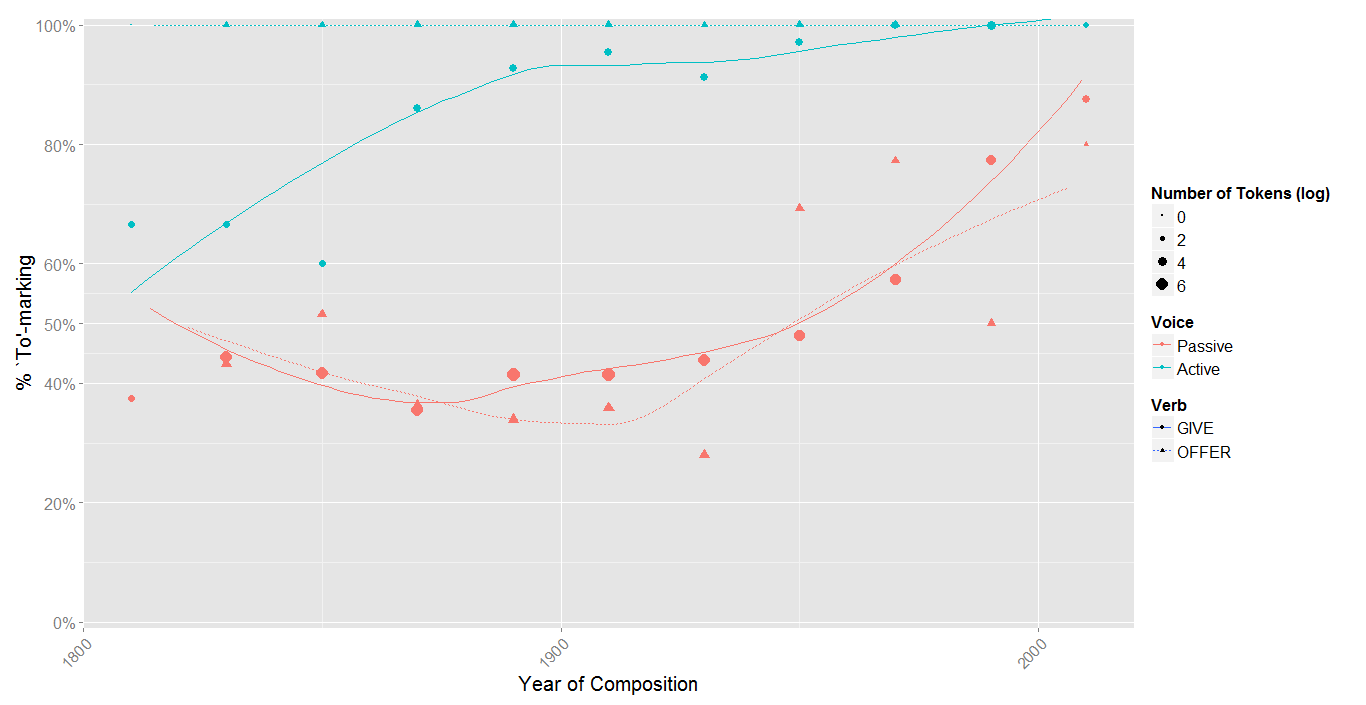
\includegraphics[width=\linewidth]{../images/recpro_to_am} 

}

\caption{LOESS lines for \textit{to} use in Modern American theme--recipient actives (with pronominal themes) and theme passives, both with pronominal recipients.\label{fig:amdata}}\label{fig:amtoset-graph}
\end{figure}

In combination with the results from Haddican's studies, this suggests that there is a complete dissociation between bare theme--recipients in the active and bare theme passives. All possible combinations of bare vs \textit{to}-marked theme--recipient actives and bare vs \textit{to}-marked theme passives are attested in different dialects/time periods. The analysis presented here predicts this dissociation, since the presence of case-based restrictions on locality are neither connected to nor solely dependent on pronoun cliticisation.

In order to investigate whether theme passives with bare recipients were restricted to theme pronouns, I extracted all tokens of theme passives with bare recipients after 1940 for a total of 337 tokens (with both full noun phrase and pronominal recipients. I coded all of the extracted tokens for the status of the theme: theme pronoun, theme noun, or theme empty (for empty categories, mostly subject relative clauses, or where information about the theme was unavailable). I found that theme nouns made up the largest number of tokens 63\%, with theme empty following at 24\%, and finally theme pronouns (almost exclusively \textit{it}) at 13\%. So, \textit{it} predominated among pronouns, probably because it is the most common theme pronoun. However, theme pronouns in general were the least likely to occur with bare recipients, probably because pronouns are rarer than full noun phrases in general in written text. The ample evidence for full noun phrase theme subjects with bare recipients reinforces the fact that bare recipients in active and passive clauses are unrelated.

To summarise, a logical conclusion on seeing theme passives with bare recipients (e.g., ``The book was given John'') would be to conclude that they derived from theme--recipient actives with bare recipients (e.g., ``I gave the book John''). In this section, I point out two problems with this conclusion. First, in Early Modern British English (and Early 19th century American English), bare recipients only occur with pronominal themes in the active but occur with full noun phrase themes in the passive. Secondly, mid-20th century American English provides an example of a language with bare recipient theme passives that lacks bare recipient theme--recipient actives. In other words, a purely locality based account of ditransitive passivisation (where theme passives always derives from theme--recipient actives) is not tenable.

\subsection{Swedish Verbs and Theme Passivisation}
As discussed above, Swedish presents one of the clearest cases for the P-incorporation analysis of dative-to-nominative conversion. In this subsection, I discuss data concerning claims that theme passivisation with bare recipients is also available with prefixed verbs. Since P-incorporation makes the recipient a valid target for subjecthood and blocks VP-internal scrambling, theme passivisation should generally be impossible in these cases, unless the recipient has moved. One type of potential counter-example that can be solved in this way are cases of purported theme passivisation with bare pronominal recipients. Cliticisation of pronominal recipients could explain why pronominal recipients can stay low in these cases.

\begin{exe}
	\ex Swedish:\label{ex:sw-offer-pass}
	\gll Ett nytt jobb erbjöds=honom.\\
A new job offered.PASS=him.OBL.\\
\trans `A new job was offered to him (\citealt{Anward.1989},\citealt{Falk.1990},\citealt{Lundquist.2006}).'
\end{exe}

If this is true, Swedish gives further clarity about the cliticisation process, since theme passivisation with unmarked recipients is \textbf{only} available with particle verbs. This suggests that in Swedish, the cliticisation process is restricted to DP pronouns. Pronouns in a dative PP (i.e., in non particle verbs) are unable to cliticise and thus serve as defective interveners for direct theme passivisation (see previous subsection).

\begin{exe}
	\ex Swedish:\label{ex:sw-give-pass}
	\gll *Ett äpple gavs honom.\\
	 An apple gave.PASS him.\\
	 \trans `An apple was given to him (\citealt{Anward.1989},\citealt{Lundquist.2006}).'
\end{exe}

However, \cite{Lundquist.2004} claims that there are examples of theme passivisation with full noun phrases with prefixed verbs.

\begin{exe}
	\ex Swedish:\label{ex:sw-offer-thepas}
	\gll Jobbet erbjöds mannen med den långa svarta kappan.\\
	job.DEF offered.PASS man.DEF with the long black coat\\
	'The job was offered to the man with the long black coat \citep[ex 26]{Lundquist.2004}.'
\end{exe}

If the prefixed verbs reflect P-incorporation, as I have argued, then direct theme passivisation is not a possible explanation (since the recipient is a valid target for subject movement). Instead, I claim that these are actually cases of recipient passivisation with theme topicalisation. Since Swedish is a V2 language, there is an ambiguity for sentence initial elements between a subject and topic interpretation. \cite{Lundquist.2004} provides examples in which themes occur in unambiguous subject positions (i.e., between an auxiliary and the passive participle) and such examples are degraded.

\begin{exe}
	\ex Swedish:\label{ex:sw-relpass}
	\begin{xlist}
		\ex[ ]{\gll Mannen som erbjöds \textbf{jobbet} hade redan tackat ja till ett annat jobb.\\
		man.DEF who offered.PASS \textbf{job.DEF} had already thanked yes to a other job\\
		\trans `The man, who was offered the job, had already accepted another job \citep[ex. 51]{Lundquist.2004}.'}
		\ex[??]{\gll Mannen som \textbf{jobbet} erbjöds hade redan tackat ja till ett annat jobb.\\
		man.DEF who \textbf{job.DEF} offered.PASS had already thanked yes to a other job\\
		\trans `The man, to whom the job was offered, had already accepted another job \citep[ex. 52]{Lundquist.2004}.'}
	\end{xlist}
\end{exe}

Another piece of evidence comes from the distribution of recipient and theme passivisation in corpora. \cite{Lundquist.2004} shows that recipient passivisation is extremely prevalent in modern Swedish (with prefix verbs), while theme passivisation is quite rare. This difference is explained if purported examples of theme passivisation are actually cases of theme topicalisation, which is expected to happen at relatively low rates in a corpus.

One challenge for this view is that there are cases where the recipient seems to not (obligatorily) occur in subject position. Since Swedish generally requires expletives when the subject position is not filled, this analysis would require that null expletives be licensed in theme relative clauses. 

\begin{exe}
	\ex Swedish:\label{ex:sw-relpass2}
	\begin{xlist}
		\ex[ ]{\gll Jobbet som erbjöds \textbf{mannen} var mycket slitsamt.\\
		job.DEF which offered.PASS \textbf{man.DEF} was very tiring\\
		\trans `The job, which was offered to the man, was very tiring \citep[ex. 49]{Lundquist.2004}.'}
		\ex[ ]{\gll Jobbet som erbjöds \textbf{mannen} var mycket slitsamt.\\
		job.DEF which \textbf{man.DEF} offered.PASS was very tiring\\
		\trans `The job, which the man was offered, was very tiring \citep[ex. 50]{Lundquist.2004}.'}
	\end{xlist}
\end{exe}

Interestingly, \cite{Haddican.2015} note that although theme passives with null recipients are generally judged unacceptable in American English, theme relative clauses are often judged much better. Since the relationship between theme relative clauses and bare recipients is replicated across at least two languages, it seems worthy of further research into the relationship between the head of relative clauses and the internal properties of the clause. However, such an investigation of relative clause structure is outside the scope of this dissertation.

\begin{exe}
	\ex Modern American English (Recipient Relatives):\label{ex:amen-relpass}
	\begin{xlist}
		\ex[ ]{The man, who was given the book, read.}
		\ex[?]{The man, who the book was given to, read.}
		\ex[??]{The man, who the book was given, read.}
	\end{xlist}
	\ex Modern American English (Theme Relatives):\label{ex:amen-rellpass2}
	\begin{xlist}
		\ex[?]{The book, which the man was given, was red}
		\ex[ ]{The book, which was given to the man, was red}
		\ex[??]{The book, which was given the man, was red}
	\end{xlist}
\end{exe}

In summary, Swedish has been claimed to allow bare recipient theme passives with prefixed verbs. Since I claim that bare recipient theme passives reflect direct theme movement past a PP recipient and that prefixed verbs in Swedish reflect P-incorporation creating a DP recipient, this data would contradict the claims I am making here. In this subsection, I argued that the Swedish data that had been used to make this claim was actually ambiguous with a theme topicalisation analysis and that data about themes in unambiguous subject position suggests that theme passivisation is not compatible with prefixed verbs in Swedish. Finally, this requires that some clauses in Swedish (especially relative clauses) may not have anything in subject position. Explaining where languages require filled subjects and where they do not is too far from the central point of this dissertation, but I also point out that similar patterns in relative clauses have been noticed to occur in American English.

\section{Conclusions}
This chapter analysed passivisation of recipient ditransitives. P-incorporation converted dative recipients into unmarked DPs, licensing dative-to-nominative conversion. This incorporation was seen on the surface in Dutch, German and Swedish. Oblique subjects were analysed by splitting the movement and case assignment properties of T into different searches (with different domains of application). In addition, surface theme passivisation with nominative themes were shown to arise from a number of possible mechanisms for avoiding locality violation, namely: relativised minimality, VP-internal scrambling, and recipient scrambling/cliticisation. Relativised minimality was argued to result in direct theme passivisation, where the theme moved to subject position directly from its base merged position.

%\bibliography{diss}

%historical case study
\chapter{Case Studies in English Diachrony}\label{ch:diachron}
\section{Introduction}
This chapter supports the claims made in the previous three chapters with three case studies in the development of recipient ditransitive syntax in the history of English. The first case study examines changes in the realisation of the dative P head. The second case study examines recipient passivisation. The third deals with the rate of passivisation from underlyingly RT (recipient--theme) word orders. As discussed in the introduction, quantitative (and especially) diachronic studies can provide a useful independent verification of analyses developed on the basis of acceptability judgements. Crucially, data from systematic patterns in language production can provide independent verification of theories developed primarily from language comprehension (i.e., acceptability judgements). This chapter begins with an introduction to the quantitative study of historical syntax, focussing primarily on statistical methods of extracting information from quantitative data. This background section is followed by a discussion of each of the case studies mentioned above. The conclusion summarises the case study results and considers broader implications for work on diachronic syntax.

\section{Quantitative Study of Historical Syntax}\label{sec:log-reg}
	Under the (commonly adopted) Borer--Chomsky Conjecture \citep{Baker.2008}, syntactic variation is driven by features of functional lexical items. Under this system, the syntactic machinery is universal and differences in the lexicon of functional items are the only points of syntactic variation. The presence/absence of a syntactic operation is formally implemented as the presence/absence of a particular feature on a functional head. Thus, syntactic change involves the addition, removal or replacement of functional items in the lexicon.

	Morphological change (especially with respect to allomorphy) can be thought of in similar terms. This analogy can be seen in the Distributed Morphology (DM) formalism \citep{Halle.1993}. In DM, allomorphy is captured by the use of vocabulary items, which formalise the relationship between syntactic/semantic features and phonological forms. Each vocabulary item must contain a set of syntactic/semantic features and a phonological form (e.g., /z/ $\leftrightarrow$ [+pl] for English plurals). A vocabulary item can also contain a context in which the item applies (e.g., /n/ $\leftrightarrow$ [+pl] / [OX,\dots]$^{\smallfrown}$\_ captures the allomorphy in plural suffixes producing English \textit{oxen}). The Subset Principle of DM (related to Panini's Elsewhere Principle) states that when multiple vocabulary items could apply (for example the contextual conditions of both the regular /z/ and irregular /n/ forms are met with the root OX), the more specific item is used (in this case the irregular /n/ form). Changes in allomorphy, thus, reflect the addition, removal or replacement of vocabulary items.

	Both syntactic and morphological changes have two stages. In order for the change to begin, some language user needs to innovate a new form, in a process called \textit{actuation}. Once a change has been actuated, the new form then needs to spread. Other speakers need to adopt the form, and speakers need to use the form more and more frequently. The increase in use frequency of the forms has been attributed to the process of grammar competition.
	
	Grammar competition occurs when two items compete to fulfil the same pragmatic function. Given that the pragmatic function of the items is the same, a speaker has no a priori way of choosing between the two items. This creates a situation of grammar competition, where two equal (or nearly equal) options are competing for use in speakers productions \citep{Kroch.1989}. A frequent outcome of this competition, diachronically, is that a newer alternatives replaces an older alternative, i.e., that over time the probability of the newer alternative continuously increases at the expense of the older alternative. Note that while the two alternatives reflect differences within the grammatical system, after the new alternative is innovated, the remaining change occurs within the non-grammatical system (i.e., is a change in the probability distribution over grammatical alternatives).

	These changes have been traditionally studied (since \citealt{Kroch.1989}) using \textit{logistic regression}, which is the standard statistical method to study variation in probabilities (i.e., numbers that range from 0 to 1). For syntactic change, the relevant probabilities are the probability of the surface form produced by the new item in any given year/context (i.e., the number of examples of the new form produced in a given year divided by the total number of opportunities to use either the old or new form). Year usually reflects the year the text was composed (assuming that the text is representative of the language for that year). The contexts reflect other factors that influence the probability of the different possible items being used (e.g., the pronoun vs. full noun status of arguments).

	Logistic regression maps the log odds\footnote{For any probability $p$, the log odds are defined as $log(\frac{p}{1-p})$.} (which range from -$\infty$ to $\infty$) to probabilities (which range from 0 to 1) using the following function: $p=\frac{1}{1+\text{exp}(-(\text{log odds}))}$. The log odds can then be modelled using linear regression, for which there are well understood methods for fitting to data. Linear regression models the value of a dependent variable (e.g., height) as the sum of weighted independent variables (e.g., age and gender). The weighting is done by multiplying each of the independent variables by a constant (called a regression coefficient). The goal of linear regression is to find the value for the regression coefficients that causes the sum of the weighted independent variables to best predict the dependent variable (for the data being modelled).

	There are three relevant types of regression coefficients for quantitative investigation of syntactic change using logistic regression. All models include an \textit{intercept}, which (for logistic regression) captures the average probability when all of the dependent variables are zero (for syntactic change this usually means for year 0 for some subset of syntactic contexts). The next type of regression coefficient are \textit{simple effects}, which for syntactic change indicate the effect of moving from one year to the next or from one context to another. The final type of regression coefficient are \textit{interactions}, which for syntactic change indicate how either the effect of year is different between different contexts or how the effect of one context is different based on some other context (e.g., how the effect of the recipient being a pronoun may be different depending on whether the theme is a pronoun or a full noun phrase).

	Modern statistics provides two main paradigms for examining regression coefficients: Null Hypothesis Testing and Bayesian Inference (this discussion and the Bayesian Inference paradigm draws heavily on the discussion in \citealt{Kruschke.2010}). While both paradigms have their origins in the 19th and early 20th century, Null Hypothesis Testing became prevalent because it was possible to easily calculate the relevant test statistics by hand (or at least by looking up the relevant values in tables). The Null Hypothesis Testing paradigm relies on asking a single question for each regression coefficient, namely is the data consistent with this coefficient being zero? Bayesian Inference instead asks: what values for the regression coefficient are plausible given the data and our prior beliefs about how systems of this type behave? Bayesian Inference provides a more nuanced approach to studying phenomenon and highlights the inherent uncertainty that underlies empirical investigation (i.e., the more data we have the smaller the range of plausible values is, but it would take an infinite amount of data to identify the exact value). This dissertation uses Bayesian Inference, and will report the 95\% uncertainty interval (i.e., the range of values such that there is a 95\% chance that the real value is above the lower bound and a 95\% chance the real value is below the higher bound).\footnote{In general the recommendations of \cite{Gelman.2008} have been followed in selecting prior distributions and in the choice of uncertainty intervals.}

	One of the major discoveries coming from the quantitative study of diachronic syntax has been the Constant Rate Effect \citep{Kroch.1989,Kroch.1994}. This effect obtains when considering a change that applies in multiple syntactic contexts. In these cases, it has been repeatedly found that the effect of year fit by logistic regression is constant across its different syntactic contexts (this is true even in cases where the environments themselves show different frequencies of use). Practically speaking, this means that significant interactions between year and variables representing syntactic contexts are not found.

	Note that the Constant Rate Effect relies on detecting a null effect (i.e., the \textit{absence} of a significant interaction). There is a statistical problem with interpreting the lack of a significant interaction in the model as reflecting a lack of interaction in reality, namely that all Null Hypothesis Testing can do is indicate whether there is sufficient data to reject the null hypothesis (i.e. that there is no interaction in reality). Thus, the lack of a significant interaction could reflect either: (a) the absence of an interaction in reality or (b) the absence of enough data to detect a real interaction. One solution to this problem is to take two further steps: (i) decide how large an effect would need to be to be considered substantial\footnote{It would take an infinite amount of data to detect that an interaction is exactly 0. However, if the effect of the interaction is really 0.00001, it would be safe to conclude that the interaction is practically non-existent. Here judgement is necessary to decide what size effect should be considered large enough that it would not be reasonable to ignore it.} and (ii) demonstrate that the data is sufficient to detect an interaction of that size. If the data set is at least as large as determined in (ii) and an interaction is still not detected, the conclusion can then be drawn that the interaction is unlikely to be substantial enough to count as a counterexample to the Constant Rate Effect. 
	
	One of the advantages of moving to Bayesian Inference is that the degree of uncertainty is built into the inference results. Since the end result of Bayesian Inference is the range of plausible values, the Constant Rate Effect simply means that zero is within the range of plausible values for the interaction between year and context. The width of the range depends on the amount of data, so the reported range demonstrates not only whether or not the data is compatible with the Constant Rate Effect, but how well it exemplifies the Constant Rate Effect (i.e., how close zero is to the boundary of plausible values and how wide the uncertainty interval is).

	Note that if there is only a small amount of data, the lack of power simply means that a larger difference in slopes would still appear as an instance of the Constant Rate Effect. Therefore, even low powered examples of the Constant Rate Effect still provide some evidence that the effect exists, the evidence is simply of low quality. Each additional example of the phenomenon, even if each example is not particularly powerful in its own right, increases our confidence that \textbf{if} the slopes really were different across contexts in the same change, the differences must be \textbf{reasonably small}, since large differences should show up even in low powered studies and smaller differences should occasionally be detected in a low powered study. The effect of low power is to decrease the probability of detecting an effect that really exists, however even if the probability of detecting the small real effect is low in any given study, the probability that the effect will not be detected decreases with each subsequent study. This happens for the same reason that rolling a 6 on a six sided die is not particularly likely, but the probability of rolling a 6 in 100 rolls of a six sided die is almost certain.

	The first example of the Constant Rate Effect comes from \cite{Kroch.1989}, where the use of do-support was studied in a number of different environments (e.g., negative declaratives, affirmative questions, negative questions, imperatives, etc.). Kroch found that while the frequency of the use of do-support in these environments differed from one another in any given year (see Fig. \ref{fig:kroch-graph}), the rate at which these frequencies changed was constant across environments (i.e., there was no significant interaction between year and the variables representing the different contexts of do-support). He hypothesised that this effect reflected the fact that only one change was taking place (the loss of V-to-T raising). Under this hypothesis, the Constant Rate Effect provides a means of recovering underlying grammatical information from diachronic patterns in language use. If a Constant Rate Effect is found (assuming that one has enough data that it would be possible to fail to find it), the most parsimonious hypothesis is that a unified change underlies the variation in each environment (i.e., use of a single new functional item is increasing in frequency).

	\begin{figure}[ht!]
		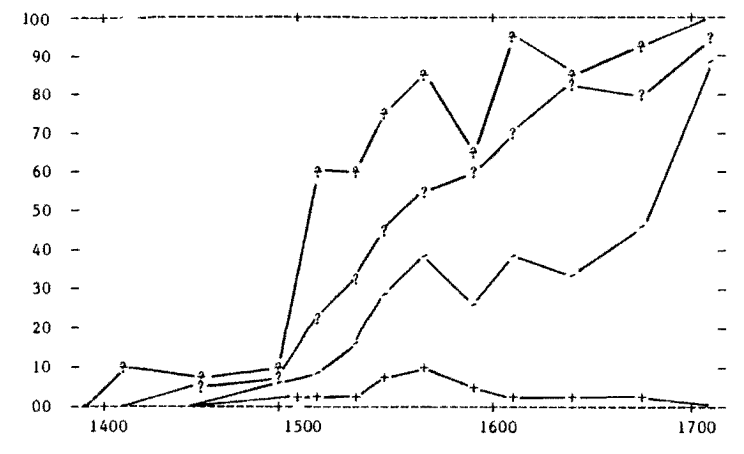
\includegraphics[width=.8\linewidth]{output/images/kroch-graph}
		\caption{Frequency of do-support in different environments: affirmative and negative questions (? and \sout{?}) and affirmative and negative declaratives (+ and ') (Fig. 1 from \citealt{Kroch.1989})}
		\label{fig:kroch-graph}
	\end{figure}

	In summary, quantitative diachronic syntax relies on logistic regression models to provide statistical comparison between various changes. The Constant Rate Effect occurs when a change spread through at least two different syntactic contexts at the same rate. This effect can be identified by the lack of a significant interaction between variables representing the different contexts and the variable representing year of composition. The interpretation of the Constant Rate Effect is that in such cases there is one grammatical change that has reflexes in multiple contexts, which means that quantitative corpus data can reveal information about the structure of the grammatical architecture (namely whether or not two surface constructions share an underlying grammatical derivation).

\section{Recipient Marking}
\subsection{Dative P Allomorphy}
This section shows how data from the history of English supports the allomorphy analysis of dative shift. As discussed in Chapter \ref{ch:active}, dative shift is the modern English phenomenon, where the recipient is unmarked when adjacent to the verb (e.g., ``John gave Mary the ball''), but marked with \textit{to} elsewhere (e.g., ``John gave the ball to Mary''). This can be captured with the pair of vocabulary items in (\ref{ex:eng-ds-vi}). This section shows how this grammar arose in the history of English. In order to support the claim that the absence of recipient marking in sentences like ``John gave Mary the ball'' reflects null allomorphy of the P head, I report a finding of the Constant Rate Effect. In particular, I provide evidence for a uniform To Item across all recipient contexts.  

	\begin{exe}
		\ex Examples:
		\begin{xlist}
			\ex John gave (*to) Mary the book.
			\ex John gave the book *(to) Mary.
		\end{xlist}
		\ex Vocabulary Items:\label{ex:eng-ds-vi}
		\begin{xlist}
			\ex Null Allomorph Item: /$\emptyset$/ $\leftrightarrow$ [dative P] / verb$^{\smallfrown}$\_
			\ex To Item: /tu/ $\leftrightarrow$ [dative P]
		\end{xlist}
	\end{exe}

	In order to study the use of \textit{to} for dative P in previous stages of the language, I extracted all tokens from the Parsed Corpora of Historical English \citep{Kroch.2000,Taylor.2003,Kroch.2004,Taylor.2006,Kroch.2010} containing the following recipient introducing verbs (verbs that also introduce goals, e.g., SEND, were excluded): ALLOT, APPOINT, ASSIGN, AYEVEN, BEHIEGHT, BEQUEATH, BETAKE, DAELAN, FEED, GIVE, GRANT, LEND, OFFER, OWE, PAY, PROFFER, PROMISE, RESTORE, SELL, SELLAN, SERVE, SHOW, VOUCHSAFE, and YIELD. I also extracted information about whether the arguments were full noun phrases or pronouns, the relative order of the recipient and theme (and their order with respect to the verb to rule out cases of topicalisation), and whether or not the recipient was marked with \textit{to} (passive data was also collected, which is discussed in Section \ref{sec:en-pas}).\footnote{See Appendix A for links to the queries used in collecting this data.} While I delay a detailed quantitative examination of the corpus results till the next subsection, Figure \ref{fig:to-use} shows the raw frequency of \textit{to} in various time phrases as well as the predicted frequencies according to the optimal model discussed in the next subsection. In this subsection, I provide a qualitative summary of the different stages of English. Since the availability of cliticisation makes data from theme pronouns more complicated, in these two subsections, I focus on cases with full noun phrase themes (e.g., ``John gave Mary the book''). I return to the case of theme pronouns in Section \ref{sec:act-tp}.

	\begin{figure}[ht!]
		\includegraphics[width=\linewidth]{output/images/to-use}
		\caption{Predicted frequency of \textit{to} with full noun phrase themes according to optimal model with raw means shown as points}
		\label{fig:to-use}
	\end{figure}

	None of the vocabulary items in (\ref{ex:eng-ds-vi}) were inherited from Old English. Old English had synthetic dative case marking, where the dative P head was realised as null (\ref{ex:old-eng-vi}), but its features were copied onto elements of the noun phrase through concord and realised on determiners, adjectives and noun heads as synthetic dative case. A consequence of the concord is that even though dative P was itself not realised phonologically, its features were phonologically realised on elements in the noun phrase. 
	\begin{exe}
		\ex Examples using Both Word Orders:
		\begin{xlist}
			\ex \gll and sealde healfne dael (*to) \TH am gesaeligan \TH earfan\\
			and gave half portion.ACC to the.DAT blessed.DAT needy.DAT\\
			\trans ` and gave a half portion to the blessed needy (coaelive.03,+ALS\_[Martin]:69.6009)'
			\ex \gll Man sceal eac syllan (*to) \TH am seocan men husel\\
			one should also give to the.DAT sick.DAT man.DAT eucharist.ACC\\
			\trans `One should also give the sick man eucharist (coaelhom.03,+AHom\_11:177.1583)'
		\end{xlist}
		\ex Vocabulary Items (6th--11th Centuries):\label{ex:old-eng-vi}
		\begin{xlist}
			\ex Universal Null Item:  /$\emptyset$/ $\leftrightarrow$ [dative P]
		\end{xlist}
	\end{exe}
	
	By the end of the Old English period (11th century), the morphological distinction between accusative and dative case inside the noun phrase was breaking down (i.e., the concord between the P head and elements in the noun phrase was no longer being clearly marked). Case marking on nouns, adjectives and determiners was no longer reliable. Both accusative and dative pronominal forms were still being used, but the forms were no longer consistently associated with dative and accusative case (i.e., old dative case forms would be used where previously accusative case was required and vis-a-versa). Around this time, \textit{to} began to be used for the first time to introduce recipients. In Old English, \textit{to} had previously been restricted to goals and addressees, i.e., the indirect object of verbs of communication \citep{Allen.1999,McFadden.2002,OED.2013}. 
	
	Under the analysis proposed here, language learners do not need to learn the existence of the dative P head, since it is always present in recipient constructions. Language learners do need to learn how the P head is realised. In Old English, the syntactic/semantic content of the P head was realised through concord on elements of the noun phrase. When the concord elements were lost, there was no longer any overt realisation of the recipient theta role. The fact that learners quickly reanalysed the goal marking \textit{to} as the realisation of a recipient P head shows that learners \textbf{proactively} seek realisations for syntactic/semantic content. In other words, a grammar with no overt marking of the recipient theta role is a possible natural language grammar (it was produced by adults in the 11th and 12th centuries), but it is diachronically unstable, because the language learning algorithm is biased towards assigning overt realisations to universally provided syntactic/semantic content, such as the recipient P.

	This reanalysis of goal \textit{to} as a possible recipient marker provides the first change in recipient marking, by introducing the To Item into the list of potential vocabulary items for speakers of English. The new grammar of English after the introduction of the To Item is shown in (\ref{ex:simple-vis-eng}). Since neither of the vocabulary items are more specific than the other, and both realise the same syntactic/semantic features, the grammar is unable to determine which item to use, which is the classic situation of grammar competition. As shown in Chapter \ref{ch:active}, the use of \textit{to} in RT orders (\ref{ex:mideng-rt-to}) cannot be attributed to Heavy NP shift, but must reflect underlying use of \textit{to} in RT orders, which supports the idea that both $\emptyset$ and \textit{to} were unrestricted in distribution). 
	\begin{exe}
		\ex Examples of Both Word Orders (spelling modernized and obsolete words translated in parentheses):
		\begin{xlist}
			\ex I have given \textbf{Purry} a gown (PASTON,I,232.2716)
			\ex They gave \textbf{to the people} this bread (CMWYCSER-M3,248.452)\label{ex:mideng-rt-to}
			\ex Thou givest thine aught (possessions) \textbf{God} (CMVICES1-M1,37.437)
			\ex Lord, in thy will, thou gave virtue \textbf{to my fairness} (CMEARLPS-M2,32.1360)
		\end{xlist}
		\ex Vocabulary Items (11th--14th Centuries):\label{ex:simple-vis-eng}
		\begin{xlist}
			\ex Universal Null Item: /$\emptyset$/ $\leftrightarrow$ [dative P]
			\ex To Item: /tu/ $\leftrightarrow$ [dative P]
		\end{xlist}
	\end{exe}

	The unrestricted distribution of \textit{to} and $\emptyset$ lasted until the 14th century. Throughout this period, \textit{to} use was more frequent in TR (theme--recipient) contexts (e.g., ``John gave the book (to) Mary'') than in RT contexts (e.g., ``John gave Mary the book''). If the recipient use of \textit{to} came from a reanalysis of the goal use of \textit{to}, this would explain the order asymmetry, since goal \textit{to} (as a traditional prepositional object) is base merged as a complement of the main verb and has the end of the verb phrase as its default word order. Our prediction of this explanation is that the TR/RT asymmetry should be insensitive to OV vs. VO word order, since the verb adjacency constraint is a later development that is used to explain the asymmetry by later language learners, rather than the origin of the asymmetry. This prediction is validated in Dutch, which has OV word order, but shows the same TR/RT asymmetry as Middle and Early Modern English.
	
	By the end of the 14th century, \textit{to} has become categorical in the TR order, while it still alternates with $\emptyset$ in the RT order. Once $\emptyset$ has become sufficiently rare in the TR order, some learners will by chance receive input with no examples of $\emptyset$ in TR orders (i.e., *``John gave the book Mary''). If the TR order was the only context recipients occurred in, then the grammar of English could have been reduced to having a single Vocabulary Item (the To Item). However, a Null Vocabulary Item is still necessary in order to account for the availability of $\emptyset$ in RT orders (e.g., ``John gave Mary the book''). In order to interpret the variation between 100\% \textit{to} use in the RT context and 50\% \textit{to} use in the RT context as a \textbf{grammatical} feature, children needed to find a local contextual clue to trigger the allomorphy (see the discussion above for the locality constraints on contextual allomorphy). Because Early Modern English had VO word order, the recipient was frequently linearly adjacent to the verb in RT orders. Thus, the RT order was able to be reanalysed as a grammatical condition of verb adjacency. The subsequent loss of verb raising in English (as part of the rise of do-support) removed the final exceptions to this generalisation (namely adverbial interveners between a finite verb and the recipient, e.g., ``John gave quickly Mary the book"). This adjacency to the verb was interpreted as a contextual cue for the distribution of $\emptyset$. The default realisation of [dative P] became \textit{to} and $\emptyset$ was restricted to a contextually specified allomorph. While this allomorph was actuated in the 14th century, it took until the 18th century for it to go to completion. During this 400 year period, the To Item was an invariable part of the grammar, but the Null Allomorph Item was only variably included in the list of Vocabulary Items. This state of affairs is presented formally in the following example:

	\begin{exe}
		\ex Vocabulary Items (14th--18th Centuries):
		\begin{xlist}
			\ex (Null Allomorph Item: /$\emptyset$/ $\leftrightarrow$ [dative P] / verb$^{\smallfrown}$\_)
			\ex To Item: /tu/ $\leftrightarrow$ [dative P]
		\end{xlist}
	\end{exe}

	The list of Vocabulary Items during the 14th--18th Centuries is identical to that of the modern grammar. The difference between the two grammars is that during the earlier period the Null Allomorph Item was only variably used. In other words, the Null Allomorph Item competed with the absence of a Vocabulary Item. This competition reflects the fact that \textit{to} was still used in the RT order during this time period. By the middle of the 18th century, the use of \textit{to} in RT contexts is the same as in the modern grammar (i.e., only grammatical when derived via Heavy NP Shift). If learners simply adopted the Null Allomorph Item wholesale, the rate of \textit{to} use in RT contexts would have instantly dropped to modern levels. As will be shown in detail in the next subsection, the rate of \textit{to} slowly decreased over the subsequent four centuries to reach modern levels.
	
	The competition of the Null Allomorph Item (122a) with the absence of an item reflects a case of \textbf{specialisation}. In Middle English, $\emptyset$ and \textit{to} were competing for the realisation of the recipient preposition across the board. Specialisation occurred when $\emptyset$ stopped competing with \textit{to} in the TR context, because the rate of \textit{to} use in that context was indistinguishable from 100\%. At that point, the variation between \textit{to} and $\emptyset$ was grammaticalised, by actuating the Null Allomorph Item. However, the primary linguistic data had more use of \textit{to} than would be predicted by the new grammar with the Null Allomorph Item. Therefore, learners needed both the new grammar and the old grammar that \textbf{only} contained the To Item in order to capture the frequency of \textit{to} in the surrounding speech community. Note that the To Item is identical between the two grammars, the only difference is the presence/absence of the Null Allomorphy Item. Thus, the development of specialisation (where the grammar becomes more complex by introducing contextual allomorphy) is driven by the competition between the new allomorph and the absence of that allomorph.

	\cite{Wallenberg.2013} argued that grammar competition inevitably results in one of two possible outcomes: (i) one of the competitors drives out the alternatives or (ii) the grammar specialises the competitors and restricts them to different contexts. The evidence from the rise of \textit{to} in English suggests that this specialisation can be driven by a learning heuristic that disprefers variation. Once probabilistic mechanisms have been introduced into the language machinery, a real question arises if there is any need for anything beyond the probabilistic mechanisms. Any probabilistic system is capable of accounting for categorical data by assigning 100\% (or 0\%) to the relevant forms. The data presented here provides evidence for the existence of a distinction between categorical and probabilistic systems in language use with a learning bias towards categorical analyses of Primary Linguistic Data. In the 14th century, it would have been possible to maintain the 11th--14th century grammar, and simply assign a 100\% probability to the use of the To Item in the TR context and a lower probability in the RT context. However, learners were averse to having surface categorical behaviour be driven by coincidental 100\% probability, instead they interpreted the surface 100\% realisation in TR orders as evidence of categorical behaviour and constructed their grammar accordingly.

	This specialisation was possible because of the following three properties of the grammar and language use in the 14th century. The first, as already described, is the fact that the use of \textit{to} had reached nearly 100\% in the TR context. The second property is the fact that $\emptyset$ still had a substantial presence in the RT context, so it was not possible for learners to simply adopt the To Item across the board. Finally, the third property was the fact that English grammar provided verb adjacency as a context to associate the remaining $\emptyset$ forms in RT context. If English did not provide a salient trigger with the proper grammatical properties (namely consistent adjacency of the recipient preposition to the verb in the RT context), specialisation would have been impossible. This predicts that this type of specialisation should be impossible in OV languages like Dutch, since the verb will not be adjacent to the recipient and thus fail to provide a salient cue for the distribution of the $\emptyset$ form. 

	To properly test this prediction would require looking at a parsed corpus of historical Dutch, which does not exist at this point in time. However, the currently typological evidence is suggestive. Of the Germanic languages that have adopted overt realisation of the dative P head (i.e., Danish, English, Swedish, Norwegian, Dutch and Afrikaans), all of the VO languages have developed the modern English grammar (where overt realisation is obligatory in TR order and the empty set is obligatory in RT order). Dutch and Afrikaans have obligatory overt realisation in the TR context, but optional overt realisation in RT contexts (i.e., they show a similar distribution as in 14th--17th century English without the contextual cue of the verbs). The currently open question is whether the grammar is progressing towards one in which To is obligatory in all contexts, or whether they have adopted some other cue for the distribution of $\emptyset$. The answer to this question awaits the public distribution of a parsed corpus of historical Dutch.

	Returning to VO languages, we find that all of the mainland Scandinavian languages (Norwegian, Swedish and Danish) have the pattern of \textit{to} in TR contexts and no \textit{to} in RT contexts.\footnote{This same pattern is also repeated in many other languages, including with other types of theta roles. In many of these languages, the data is more problematic for my account, since the variation between overt/null preposition coincides with an alternation between overt/null applicative morphemes (see \citet{Baker.1988} for a discussion of the alternation in languages with applicative morphemes). I do not have an explanation for the applicative alternation.} Given that the synchronic explanation for this phenomenon relies on contextual allomorphy, it is non-predicted that the same allomorphy pattern would reoccur in language after language. While the analysis given here does not provide a synchronic explanation for the typological patterns, the \textbf{historical} analysis suggests an explanation. As discussed above, the RT=null/TR=overt pattern found in English was not purely the consequence of accident (e.g., series of independent phonological changes that underly many cases of allomorphy). Instead, the pattern is derived from the origin of the prepositional marker in Prepositional Object Constructions. Thus, as long as languages are deriving their prepositional objects from the same source, it is plausible that the same learning trajectory would repeat in language after language. This is similar to the pattern of common sound changes occurring over and over again producing the same surface patterns (e.g., palatalised consonants before front vowels). While the distribution of null and overt forms in the synchronic grammar is purely accidental, there are strong historical reasons to expect that the same series of accidents would occur in language after language. This claim makes a strong prediction about the historical pattern in other languages that have the RT=null/TR=overt pattern, namely that those languages would show the same rise--fall pattern seen in the history of English.

	\subsection{Quantitative Analysis of the Rise of \textit{to}}
		The previous subsection claimed that the rise in \textit{to} use during the Middle English period reflected the uniform adoption of the To Item, which applied even in RT contexts. A quantitative prediction of this analysis is that a Constant Rate Effect should be found across all contexts in this period. Data was collected from four contexts: (i) TR with recipient noun, (ii) TR with recipient pronoun, (iii) RT with recipient noun, and (iv) RT with recipient pronoun. In order to test the Constant Rate Effect, it is necessary to create a mathematical model for the rate of \textit{to} in these contexts.
	
		For the two TR contexts (with full noun phrase and pronominal recipients), this rise can be modelled with the standard logistic regression models, since they show the typical 0\%--100\% S-shaped curve. The RT contexts require a different model, since \textit{to} rises from the 11th till the 14th century and then decreases in use until the 18th century (as seen in Figure \ref{fig:to-use}). The simple mathematical correlate to the qualitative model discussed above is to use a \textbf{piecewise} function. 
	
		Using a piecewise function, different logistic equations are used depending on whether the reanalysis point in the 14th century has been reached. Up until the reanalysis point in the 14th century, this context will be modelled with a logistic equation with a positive slope (i.e., the frequency of \textit{to} should increase). A Constant Rate Effect would hold between the RT contexts and the TR contexts if the slope of the first half of the RT function is the same as the slope predicted for the TR contexts. After the reanalysis point, a new logistic equation with a negative slope would be used, which would capture the decrease in frequency of \textit{to} from the 14th through the 18th century.

	For the piecewise function, there is one more constraint that is necessary. The frequency predicted by the two equations (before and after the reanalysis point) should be the same at the reanalysis point. This equality is necessary to capture the fact that when the learners do the reanalysis the distribution of the two forms in the newly proposed grammar would be chosen so that they would match the frequencies generated by the pre-reanalysis grammar. This equivalence is captured formally by selecting intercept terms for the second equation that (given a particular slope) generate the correct frequency at the reanalysis point. Therefore, the intercepts in the second function do not need to be estimated, once the reanalysis year has been selected.

	All of the parameters were estimated using Bayesian Inference with RSTAN \citep{stan.2016}. The results of relevance to the Constant Rate Effect are presented in Table \ref{tab:to-mcmc}, where plausible values are defined as being within the 95\% uncertainty interval. As discussed above, Bayesian Inference tests for the Constant Rate Effect by seeing if zero is a plausible value (i.e., if zero is in the uncertainty interval). If zero is \textbf{not} within the uncertainty interval, then zero should not be treated as a plausible value for the interaction and the data provide evidence against the existence of a Constant Rate Effect.

\input{'output/tables/to-mcmc.tex'}

   The results reflect a number of distinct tests for the Constant Rate Hypothesis. In general, the results support two major conclusions. First, the data is consistent with the analysis presented in the previous subsection, where the early rise of \textit{to} is derived from the spread of the To Item through the grammar impacting all ditransitive constructions simultaneously. This conclusion is supported by the CRE findings between RT and TR word orders for the rise of \textit{to}. CH1 Interaction (b) shows that the data is consistent with a Constant Rate Effect in the rise of \textit{to} between sentences like "I gave the books (to) John" and "I gave (to) John the books". CH1 Interaction (d) shows an even stronger example of the Constant Rate Effect for similar sentences with pronouns (e.g., "I gave the books (to) him" and "I gave (to) him the books"). These results bolster the theoretical claims about the nature of the change given in the previous subsection.

   However, the quantitative analysis also reveals that there is a disconnect between the spread of \textit{to} between nouns and pronouns. In the previous subsection, the assumption was that nouns and pronouns behaved identically with respect to the realisation of the dative P head. The CH1 Interaction (a) shows that there was \textbf{not} a Constant Rate Effect finding between sentences like "I gave the book (to) John" and "I gave the book (to) him". The use of \textit{to} with pronouns seems to have been actuated later than its use with nouns, but then spread through the grammar quicker (as can be seen in Figure \ref{fig:to-use} on page \pageref{fig:to-use}). It was also the case that sentences like "I gave (to) him the book" behaved more like "I gave the book (to) him" than to "I gave the book (to) John", with zero on the border of plausible values for the comparison between "I gave (to) him the book" and "I gave the book (to) John" (CH1 Interaction c). Finally, the development of the null form in RT contexts did not show a constant rate effect (CH2 Interaction), with pronouns showing a faster development of the null form. Together, these three pieces of evidence suggest that recipient pronouns and recipient noun phrases reflect different morphological systems.

   Given the difference between nouns and pronouns in both changes, it would have been reasonable for the reanalysis points to be different. The data from the parsed corpora are consistent with recipient nouns and pronouns sharing the same reanalysis point. However, if there is a difference between nouns and pronouns, it is likely that pronouns had a later reanalysis point than nouns (Reanalysis Diff). This is consistent with the analysis presented above, where high rates of \textit{to} use in TR clauses drove the reanalysis in RT clauses. Since the use of \textit{to} went to completion in TR clauses later with pronouns than with full noun phrases, it was predicted that the reanalysis point for pronouns be slightly later than for full noun phrases.

   Such a difference between the morphological realisation of nouns and pronouns is not uncommon cross-linguistically. Indeed, most of the Romance languages have the property where clitic recipient pronouns have a null dative P head, while full noun phrase recipients and non-clitic pronouns have an overt dative P head (in the Romance equivalent of \textit{to}). It may be the case that the difference in English also reflects a difference between clitic and non-clitic pronouns in English. In the next sub-section, I discuss other evidence for the existence of pronoun cliticisation in English and its impact on the morphological realisation of the dative P head.
    
	\subsection{Pronoun Cliticisation}\label{sec:act-tp}
	In this subsection, I present evidence of special behaviour by pronouns, focusing of data where the theme is a pronoun. When the theme is a pronoun, the TR order was essentially categorical (31 examples of RT order over 1000 years out of 712 examples with theme pronouns). Since there was such poor evidence for the frequency of \textit{to} use in these environments, their inclusion muddled any attempts at statistical analysis. Therefore, those cases have been excluded for the analyses discussed below. Instead, I focus on cases where with a theme pronoun and a TR order.

	As discussed in Chapter \ref{ch:active}, theme pronoun cliticisation can produce surface violations of the generalisation that the null allomorph of the dative P head only occurs adjacent to the verb (e.g., ``John gave it Mary''). The theme pronoun does not intervene once it has cliticised, because it is considered morphologically to be a part of the verb. I showed that in some dialects of Northwestern British English, this process still occurred:

	\begin{exe}
		\exr{ex:nw-brit-P} Northwestern British English:
		\begin{xlist}
		\ex[ ]{John [gave=it] [P=$\emptyset$ Mary]}
		\ex[*]{John [gave] [the book] [P=$\emptyset$ Mary]}
	\end{xlist}
	\end{exe}

	The effect of theme pronoun cliticisation can also be seen in the historical data. Figure \ref{fig:brit-tp} shows data from TR word orders with theme pronouns. In both cases, the same rise in \textit{to} as discussed earlier is seen, which just shows the adoption of the To Item. However, instead of levelling out at 100\%, for both recipient noun phrases and recipient pronouns, the logistic regression goes to some point short of completion, which can be explained as reflecting the combination of adopting the Null Allomorphy Item and the rate of theme pronoun cliticisation. For full noun phrase recipients, the rate of \textit{to} use is $\sim$\input{output/tables/fnpr-dtp.tex}, while for pronoun recipients, the rate of \textit{to} use is $\sim$\input{output/tables/pr-dtp.tex}.\footnote{These reflect the average rate of \textit{to} use in these two context between 1425 and 1700.} While theme pronoun cliticisation explains the existence of null marked recipients in these contexts, it does not explain the discrepancy between full noun phrase and pronoun recipients.

	\begin{figure}[ht!]
		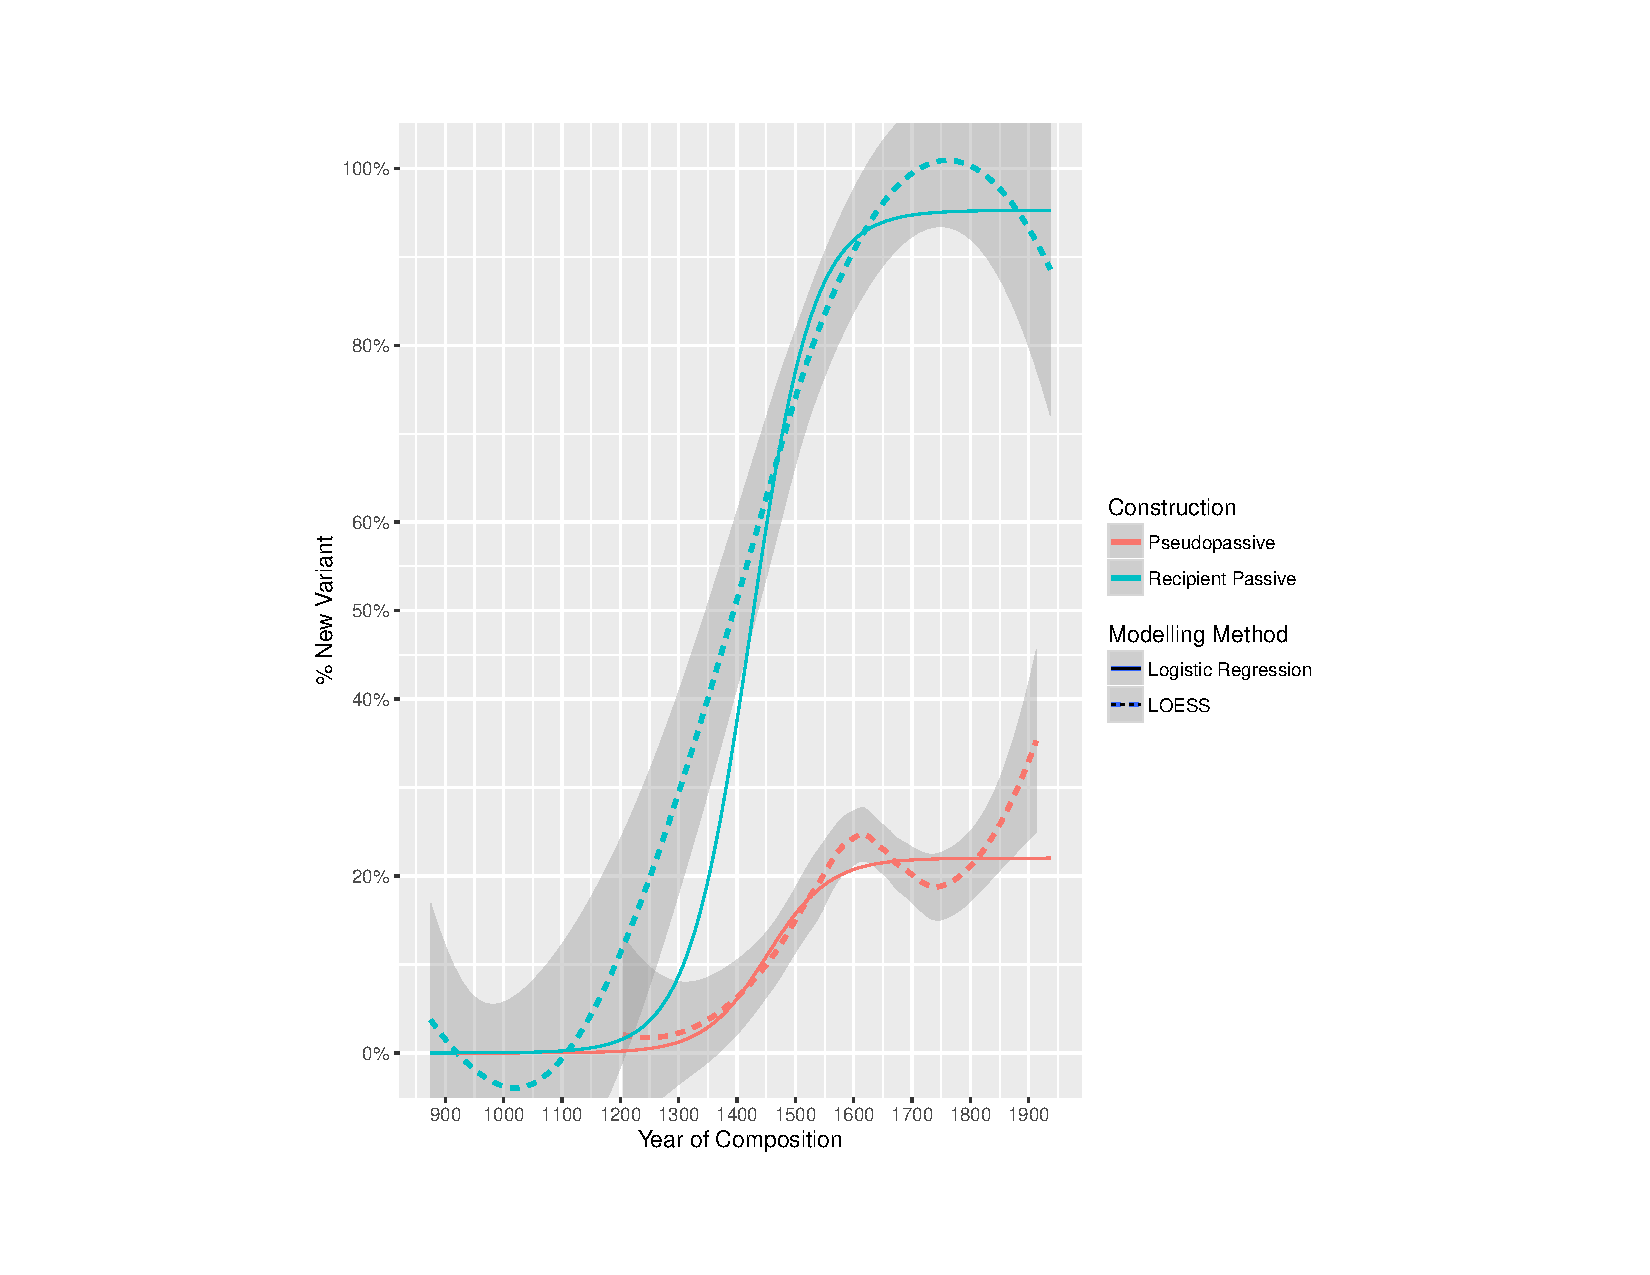
\includegraphics[width=\linewidth]{output/images/brit-tp}
		\caption{LOESS fits for TR data with theme pronouns (points indicate raw frequencies)}
		\label{fig:brit-tp}
	\end{figure}

	In the previous subsection, it was seen that pronoun recipients showed different behaviour from full noun phrase recipients in the adoption of the Null Allomorphy Item. I proposed that this involved a process of recipient pronoun cliticisation, which showed different morphological marking than full noun phrase recipients. The same explanation works for the situation discussed here. Theme cliticisation on its own is fairly rare, as seen by the low rate of null full noun phrase recipients. However, when both the theme and the recipient are pronouns, both pronouns are likely to cliticise, and the null form associated with the recipient pronoun explains the lower rates of \textit{to} use. The propensity for recipient pronouns to be null marked seen both in this subsection and the previous subsection supports the notion that the use of \textit{to} reflects morphological variation that is sensitive to pronominality as is seen in the morphological distinction between clitic and non-clitic pronouns in many Romance varieties.

	As can be seen in Figure \ref{fig:brit-tp}, the difference between pronouns and full noun phrases seems to be shrinking in standard Modern British English (i.e., after 1700). As discussed in chapter \ref{ch:passive}, American English data shows that sentences like ``John gave it Mary'' and ``John gave it him'' were already rare at the beginning of the 19th century in American English and were lost by the middle of the 20th century. While the British data ends in the early 20th century, it seems that the same process was affecting standard British English. It seems both standard British and standard American English lose pronoun cliticisation effects over the 18th, 19th and 20th centuries.

	Additional evidence for cliticisation comes from looking at recipient marking in theme passivisation and how it changes in American English. The relevant change is the loss of direct theme passivisation (e.g., ``The book was given John''), where the theme raises across the recipient to subject position (for more discussion see Chapter \ref{ch:passive}). In English, direct theme passivisation can be identified by the absence of \textit{to} before the recipient. If the theme scrambles to the left of the recipient before raising to subject position, then its lower copy intervenes between the recipient and the verb, preventing the null allomorph from being used (\ref{ex:eng-directtheme}).

\begin{exe}
	\exr{ex:eng-directtheme} English Dialects:
		\begin{xlist}
			\ex[ ]{The book was given P=$\emptyset$ the man \sout{the book}.}
			\ex[*]{The book was given \sout{the book} P=$\emptyset$ the man \sout{the book}.}
		\end{xlist}
\end{exe}
	
	In Chapter \ref{ch:passive}, direct theme passivisation was argued to result from two possible sources: (a) the locality properties of T in looking for a subject to move (i.e., are PPs valid subjects and how many arguments can T consider for subject properties) and (b) recipient pronoun cliticisation. When direct theme passivisation is possible, the recipient is passed over for subject movement either because, as a PP, it is not a valid subject and T can keep looking down the tree to find the theme or because as a clitic it has incorporated into the verbal head. In the new grammar, however, T is no longer allowed to consider multiple arguments. Therefore, the recipient blocks passivisation since T can no longer keep looking and find the theme. The loss of direct theme passivisation can be operationalised as both: (a) the replacement of T with the invisible search property with one with defective intervention and (b) the loss of recipient pronoun cliticisation. The trajectory of this change can be seen in Figure \ref{fig:loss-of-dt-in-amen} on the next page.

	\begin{figure}[ht!]
		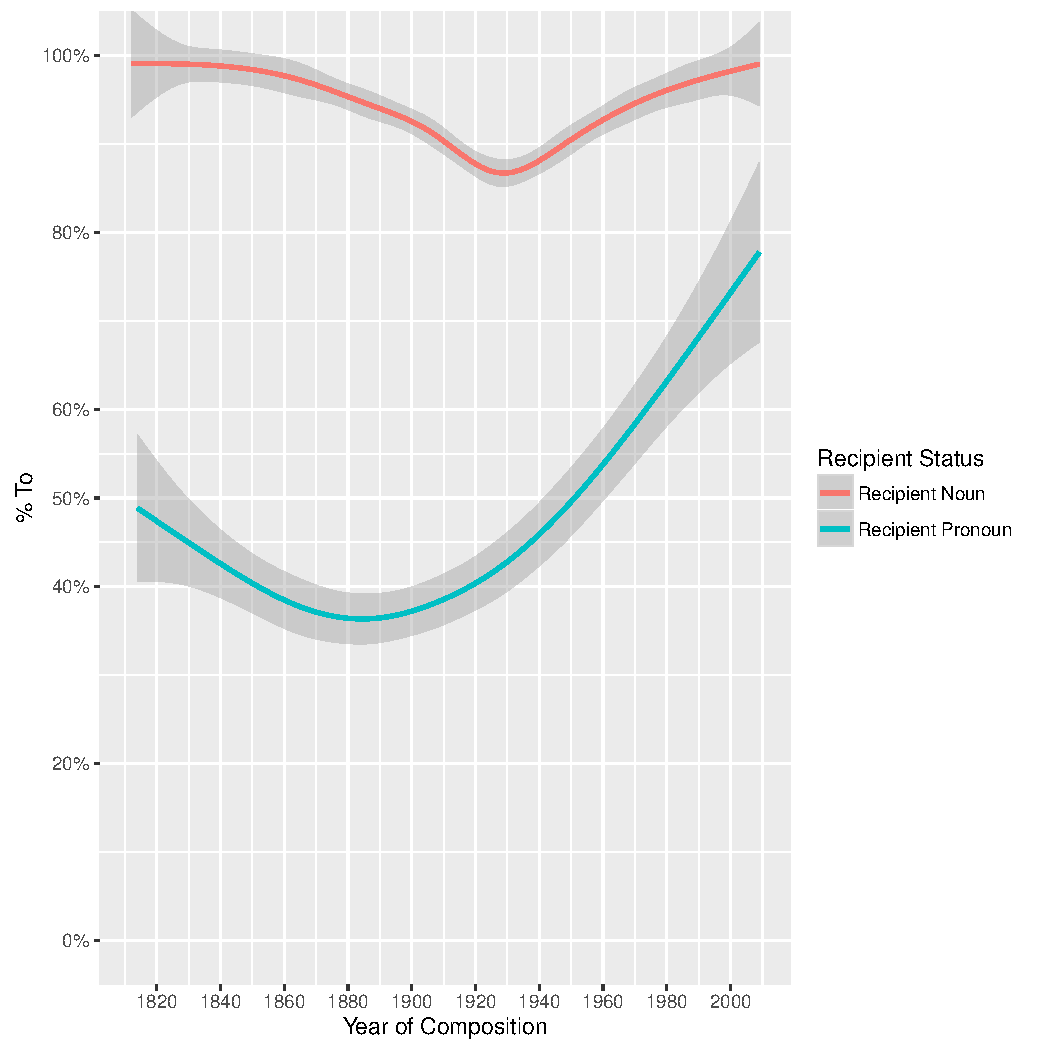
\includegraphics[width=\linewidth]{output/images/directtheme-am}
		\caption{LOESS curves showing the loss of direct theme passivisation with GIVE and OFFER in American English}
		\label{fig:loss-of-dt-in-amen}
	\end{figure}

	The rise/fall pattern seen in the development of direct theme passivisation in American English is discussed further in section \ref{sec:pasrate}. Before turning to that, it is worthwhile to spend a brief moment on the loss of recipient pronoun cliticisation. As can be seen in Figure \ref{fig:loss-of-dt-in-amen}, direct theme passives (absence of \textit{to} with theme passivisation) are much more common with pronoun recipients than full noun phrase recipients, suggesting that pronoun cliticisation was a common operation that could independently derive direct theme passivisation. The higher rates of direct theme passivisation with recipient pronouns can be directly attributed in this case to the fact that there are two independent mechanisms for generating the same surface phenomenon.
	
	In Chapter \ref{ch:passive}, I showed that direct theme passivisation survived in American English after the loss of theme cliticisation (i.e., after sentences like ``I gave it him'' became ungrammatical). While the loss of theme cliticisation and the loss of recipient cliticisation were shown to not be identical, there is a plausible connection between the two. It is plausible that language learners generalise evidence about one type of cliticisation, using the evidence of cliticisation with one type of pronoun as supporting evidence for cliticisation with other types of pronouns. Thus, the loss of theme cliticisation removed a potential source of evidence for the existence of cliticisation in the grammar. It is probably not coincidental that direct theme passivisation begins to decline around the same time that theme cliticisation is lost (i.e., 1940s).
 
	\section{Recipient Passivisation}\label{sec:en-pas}

	The change discussed in this section is the replacement of oblique passives (e.g., 'him was given the book') by nominative recipient passives (e.g., 'he was given the book'). The structure of the section is as follows. First, Old English is discussed and it is argued that the situation is too impoverished to provide clear data, although there is suggestive evidence that Old English had some oblique passives. Secondly, I discuss the change from oblique passives to nominative passives and show that this change co-exists with the rise in pseudopassivisation in English, which supports the notion that nominative recipient passivisation derives from P-incorporation as discussed in Chapter \ref{ch:passive}. 

\subsection{Old English}
	The situation in Old English is quite complex. \cite{Allen.1999} provides evidence that monotransitive datives are able to become oblique subjects in Old English and not topicalised objects. To discuss this distinction, she introduces the term ``fronted dative'', which is agnostic as to whether the fronted element is a topic or a subject. Contrary to her claims about monotransitive datives, she argues that there are no oblique subjects in ditransitive passives, only topicalised objects. This claim is made on the basis of Coordinate Subject Deletion facts. In Old English (as in Modern English), arguments are generally obligatory (i.e., neither subject nor object drop is generally licensed). However, when two sentences are coordinated and share the same subject, the subject does not need to be expressed in the second sentence (\ref{ex:OECSD}). In a corpus investigation, none of the fronted datives in ditransitive passives triggered Coordinate Subject Deletion, while a number of fronted nominatives did (see Table \ref{tab:AllenOECSD}). 

	\begin{table}[t]
		\begin{tabular}{cccc}
			Nominative Coreferential & & Deletion & No Deletion \\
			& Order NOM DAT & 11 & 4 \\
			& Order DAT NOM & 4 & 3 \\
			& Total & 15 & 7 \\
			\hline
			Dative Coreferential & & Deletion & No Deletion \\
			& Order NOM DAT & 0 & 27 \\
			& Order DAT NOM & 0 & 11 \\
			& Total & 0 & 38 \\
		\end{tabular}
		\caption{Allen's counts of Coordinate Subject Deletion with ditransitive passive in OE prose (Table 2-6, \citealt{Allen.1999})}
		\label{tab:AllenOECSD}
	\end{table}

	\begin{exe}
		\ex \label{ex:OECSD} Old English:
		\gll and him comon \textbf{englas} to, and him ðenodon\\
		and him.DAT came \textbf{angels.NOM} to, and him.DAT served\\
		\trans ` and to him angels came and him (they) served \citep[ex. 34]{Allen.1999}.''
	\end{exe}

	The main problem with this conclusion is that there were only a small number of Old English coordinated examples, such that the lack of deletion for datives could be accidental. The problem of whether fronted oblique elements are subjects is not unique to Old English. The same uncertainty hold with respect to Old Norse (see for example \citealt{Kristoffersen.1991,Kristoffersen.1994} and \citealt{Bardal.2001b}). Unfortunately, many of the examples that clearly show that oblique elements are subjects rely on negative data, which is unavailable for earlier states of the language. Because of this problem, I focus instead on data starting with Middle English, where I make the assumption that oblique fronted elements are subjects, since Middle English has developed an obligatorily filled subject position and lost any traces of V2 (or V2-like effects), meaning that the element immediately before the finite verb is the subject.

	\subsection{Rise of Nominative Recipient Passivisation}\label{sec:eng-to-pass}

	As discussed in the previous subsection, I am assuming that Middle English has oblique subjects in cases of fronted recipients. However, since synthetic case marking had been lost (for full noun phrases) by Early Middle English and since the To Grammar (see the previous section) was not yet universal, even with these assumptions, it is difficult to determine whether a fronted recipient was nominative or dative. \cite{Allen.1999}, after carefully examining the extant Middle English corpus, identifies that the first unambiguous case of a nominative recipient subject in the passive of a ditransitive occurs in 1375. This reflects a change in the grammar of English, in so far as previously nominative recipient subjects were ungrammatical and now they are grammatical.

	There are potentially three distinct types of recipient passive. Example (\ref{ex:obliq-rec-eng}) shows an example of oblique passive without \textit{to}. Even though the recipient itself (``the king Gurthym'') is ambiguous between an oblique and nominative structure, the fact that the verb (``were'') agrees in number with the theme (``the provinces'') shows that the theme received nominative case and the recipient subject must be oblique. These kinds of examples are quite rare. Most examples of recipient subjects without \textit{to} are coded as nominative subjects (\ref{ex:nom-rec-eng}), even though their form does not distinguish between an oblique and a nominative analysis. Clear examples of oblique recipient passives can be seen in (\ref{ex:obliq-to-rec-eng}). As discussed in the previous section, the realisation of dative P as \textit{to} became obligatory for non-adjacent constructions by about 1400. At that point, the distinction between \textit{to}-marked (\ref{ex:obliq-to-rec-eng}) and bare recipients (\ref{ex:nom-rec-eng}) becomes an unambiguous indicator of the case of the recipient (namely dative and nominative respectively).

	\begin{exe}
		\ex Middle English \citep{Kroch.2000} and Early Modern English \citep{Kroch.2004}
		\begin{xlist}
			\ex\label{ex:obliq-rec-eng} the king Gurthym, that we clepteth Gurmundus, were i-yeve the provinces of Est Anglia and Northumbria (CMPOLYCH-M3,VI,377.2770)
			\ex\label{ex:nom-rec-eng} for the prioress is given a matter to proud in the beginning of her ordinance (CMBENRULE-M3,43.1346)
			\ex\label{ex:obliq-to-rec-eng} to thy holy name be given laude and praise (STOW-E2-P2,581.96)
		\end{xlist}
	\end{exe}

	Under the analysis described in Chapter \ref{ch:passive}, the nature of this grammar change reflects the availability of P-incorporation. Without P-incorporation, the only possible form of recipient passivisation is to have oblique subjects. Given that P-incorporation also generates pseudopassives, the simple prediction would be that pseudopassives would enter the language at the same time as nominative recipient passives. \cite{Sigursson.2014} showed that pseudopassivisation comes into the language in the beginning of the Middle English period. Indeed, as seen in Figure \ref{fig:recpas-pseudo}, pseudopassivisation and nominative recipient passivisation increase in use from about 1200 until 1650, when they both level off.\footnote{The pseudopassive data here is taken from a hand corrected dataset produced by Sigursson from the Parsed Corpora of Historical English. Using automatic queries, roughly the same number of pseudopassive examples are found, but the number of corresponding actives are much higher. This discrepancy probably derives from a failure to identify a number of criteria that would prevent a possible active from being a potential pseudopassiviser. Since Sigursson curated his dataset for the study of pseudopassivisation, it provides a more reliable dataset and therefore his values are reported here.}

	\begin{figure}[ht!]
		\includegraphics[width=\linewidth]{output/images/recpas-old-pseudo}
		\caption{Logistic regression curves and LOESS curves showing rates of nominative recipient passivisation and pseudopassivisation in English}
		\label{fig:recpas-pseudo}
	\end{figure}

	Neither pseudopassivisation nor nominative recipient passivisation go to 100\%. For pseudopassivisation, this is expected. If the pseudopassivisation rate was 100\% that would mean that there were no active sentences with PP objects, which is highly improbable. For nominative recipient passivisation, it is less clear why the process should not go to completion, since this is the probability of having a nominative subject given that recipient passivisation has occurred, which could reasonably occur 100\% of the time. However, locative inversion remains possible to the present day (\ref{ex:locinv}). There is debate in the literature about the proper analysis of locative inversion, but it seems likely that locative inversion is actually a type of topicalisation and not subject raising \citep{Bresnan.1994}. Ideally, locative inversion should be excluded from our cases, but this cannot be done, since cases of locative inversion are surface identical with the cases of oblique passivisation with \textit{to}.

	\begin{exe}
		\ex Modern English: To the guests were given goblets of gold and silver (\citealt{Bruening.2010}, Ex 26a)\label{ex:locinv}
	\end{exe}

	To summarise, the change from oblique passivisation to nominative passivisation suffers from two surface complications. In the early period, some cases of oblique recipient passivisation have bare recipients, since realisation of dative P as \textit{to} was not yet obligatory. Also, throughout the change, some cases of fronted recipients with \textit{to} represent cases of locative inversion, which properly should not be included, but cannot be distinguished from genuine cases of oblique recipient passivisation. In spite of these complications, it is possible to do quantitative research on the trajectory of the change.

	This change would seem to be a good case to look for a Constant Rate Effect (see Section \ref{sec:log-reg}), namely between the rise of pseudopassivisation and the replacement of oblique recipient passives by nominative recipient passives, since both are proposed to reflect the underlying adoption of P-incorporation into the grammar. However, there are two problems that impede investigation of a constant rate effect. There is a great deal of uncertainty about the rise of nominative recipient passivisation, because there are few cases of recipient passivisation overall (see the next subsection for a discussion of why there is little data). Thus, even if a Constant Rate Effect is found (i.e., there was no significant interaction between year and pseudopassive vs nominative recipient passive), this can be attributed to the lack of data concerning recipient passives. Secondly, the fact that the changes do not go to 100\% means that standard techniques for fitting the logistic regressions cannot be used.

	In order to resolve the second problem (fitting models to data that does not go to 100\%), scaled versions of logistic regression can be used, where the output of the formula for each year is scaled by multiplying the predicted output by a scaling constant reflecting the final rate of usage. For example, assume that the change from oblique recipient passives to nominative recipient passives stabilises at 90\% instead of 100\%. The rate of 90\% is calculated by averaging the rate of all years after the change seems to have stabilised (in this case after 1700). Instead of using the direct output of logistic regression to predict the probability of using a nominative recipient passive in any year, the output of the logistic model is first multiplied by 90\%. The consequence of this process is that at the end of the change the predicted probability is 90\% instead of 100\%. The optimal values for the logistic regression parameters can still be estimated from the data, so a Constant Rate Effect can still be tested for. 

	In this case, a Constant Rate Effect was found. Table \ref{tab:pas-change-tab} shows that zero is a plausible value for the Year:Type interaction. In fact, the effect here is even stronger than the Constant Rate Effect, since the data is compatible with there being no difference at all between the two conditions. Since the data from recipient passives is tentative, the result is only suggestive, but it is most consistent with the notion that the rise of nominative recipient passivisation and pseudopassivisation are derived from the same underlying change, namely the adoption of P-incorporation.

\input{output/tables/recpas-old-mcmc.tex}

	In summary, the rise of nominative recipient passives in English provides tentative additional evidence for the P-incorporation analysis. Nominative recipient passivisation and pseudopassivisation enter the language in the same way, providing another example of the Constant Rate Effect. Since P-incorporation is a standard analysis of pseudopassivisation, the Constant Rate Effect finding supports the notion that nominative recipient passivisation is also derived via P-incorporation when the operation entered the language during the Middle English period. One caveat about the Constant Rate Effect finding was that it was based on only a small amount of data from recipient passives. The next subsection discusses why there are so few recipient passive examples.

	\section{Passivisation and Underlying Word Order}\label{sec:pasrate}

	This subsection discusses a change in American English that supports the analysis of direct theme passivisation as being derived from an underlying RT word order. In particular, before the loss of direct theme passivisation in 20th century American English (as discussed above), recipient passivisation and direct theme passivisation pattern together. In Early Modern and Modern British English, they both show depressed rates, which both increase in American English. While the proper account of the depressed passivisation rate and its subsequent increase are unknown, the fact that recipient passives and direct theme passives pattern together supports the notion that they share some property in common. Under the analyses proposed here, the shared property is passivisation from the RT word order.

	As discussed in the preceding subsection, the grammar of recipient passivisation changed during the Early Modern British period from oblique recipient subjects to nominative recipient subjects. However, during that time, the over all rate of recipient passivisation (as either oblique or nominative) remained constant at about 1\% (as can be seen in Figure \ref{fig:brit-pas} on the next page), which reflects the percentage of passive sentences with RT word order out of all sentences with RT word order. This rate of 1\% is substantially lower than the rate of monotransitive passivisation and the rate of passivisation with TR word order (as shown in Figure \ref{fig:brit-pas}). Table \ref{tab:model-comp-pasrate} on the next page shows that there is a difference in passivisation rates between RT and TR word orders (i.e., 0 is not a plausible value for the difference).
	\input{'output/tables/pas-mcmc.tex'}

	\begin{figure}[ht!]
		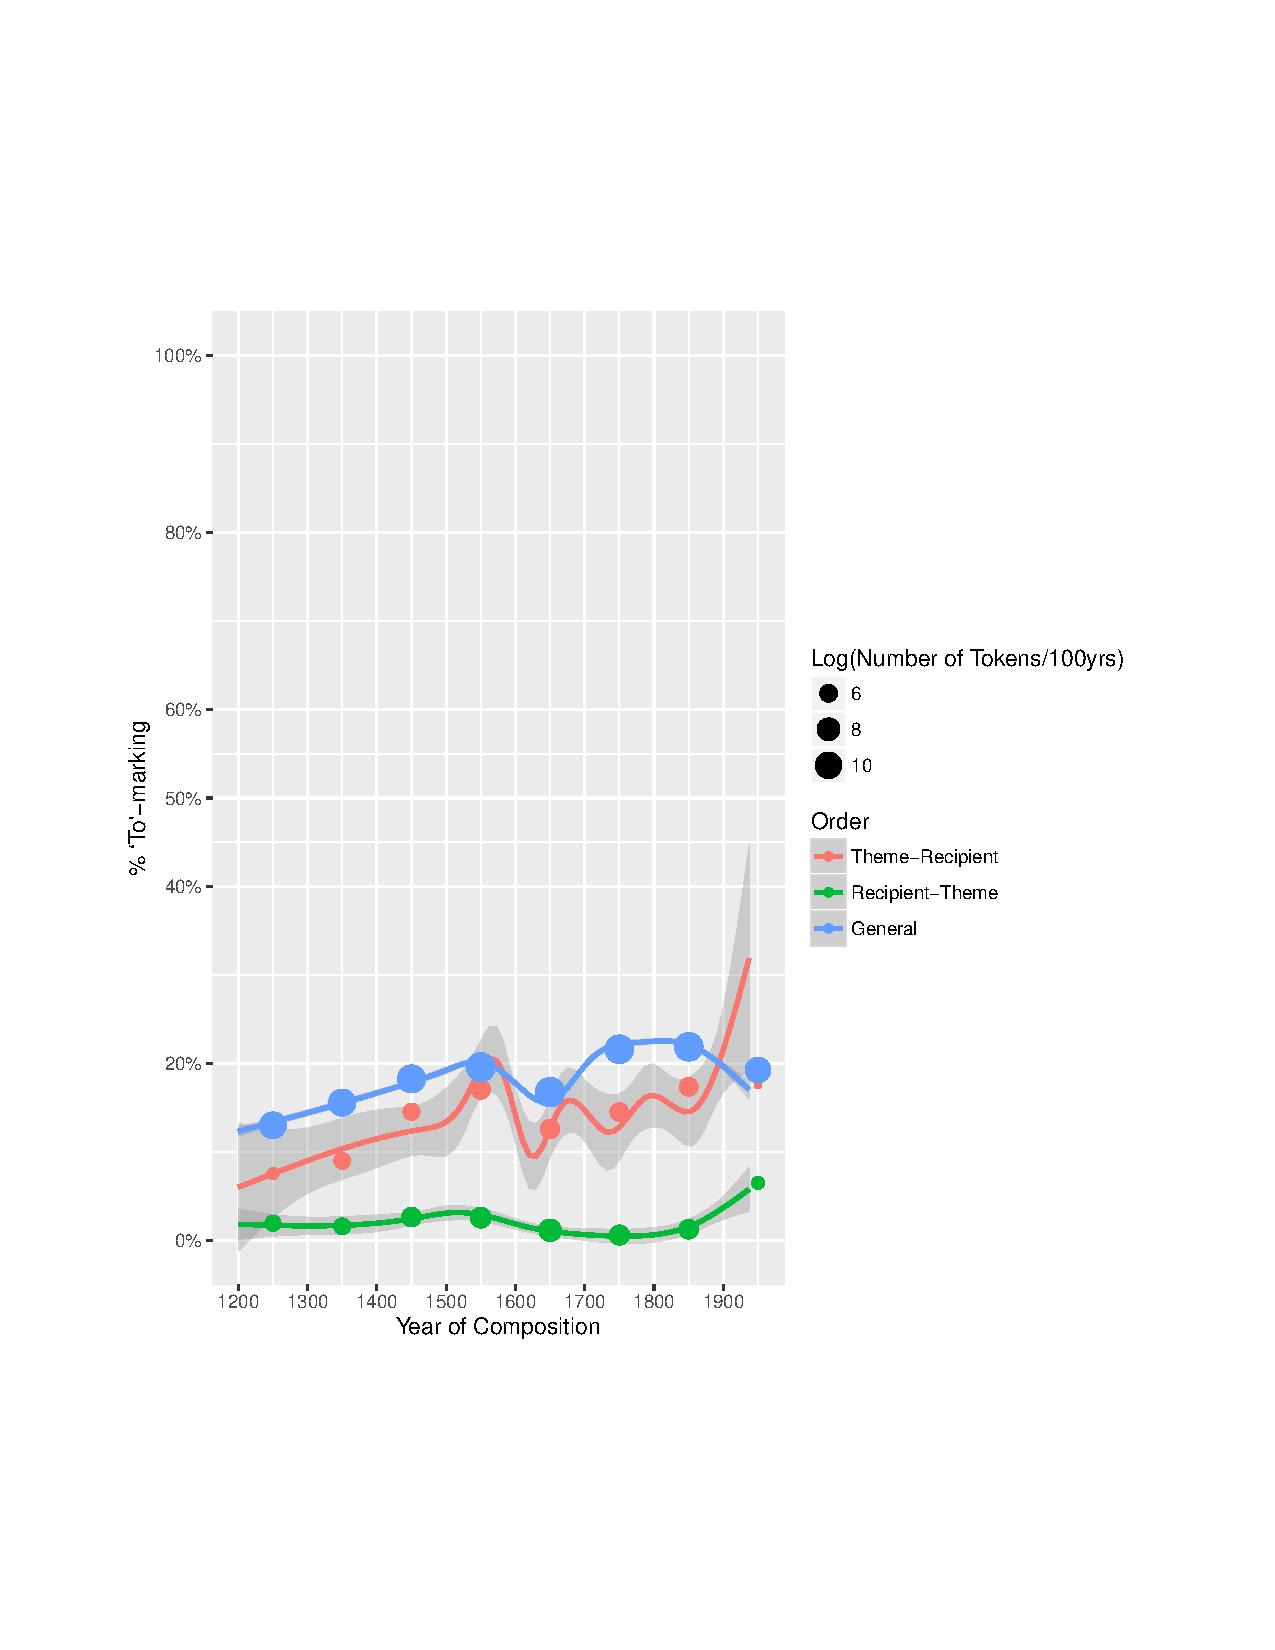
\includegraphics[width=\linewidth]{output/images/brit-pas}
		\caption{LOESS fits for rates of passivisation in TR, recipient theme and general clauses}
		\label{fig:brit-pas}
	\end{figure}

	At the same time, as shown in Figure \ref{fig:brit-tp} on page \pageref{fig:brit-tp}, the rate of direct theme passivisation (i.e., lack of \textit{to} marking on the recipient in a theme passive) with full noun phrase recipients was also low. In both cases, recipient passivisation and direct theme passivisation occur often enough that they are unlikely to be the product of errors and thus should be taken as grammatical, but seem to be seldomly used. The fact that both of these constructions show a marginal status in the British English data is not a particularly strong argument in favour of them sharing an underlying analysis. However, in American English, the marginal status of these constructions goes away at the same time. Figure \ref{fig:am-change-pass} shows the rate of recipient passivisation and direct theme passivisation together in American English with full noun phrase recipients. Throughout the 19th century (i.e., before the loss of direct theme passivisation), the rate of direct theme passivisation and recipient passivisation rise in tandem. The parallel nature of this change can be captured by assuming that whatever the formal properties of the change are, they target passivisation from RT underlying word orders.

	\begin{figure}[ht!]
		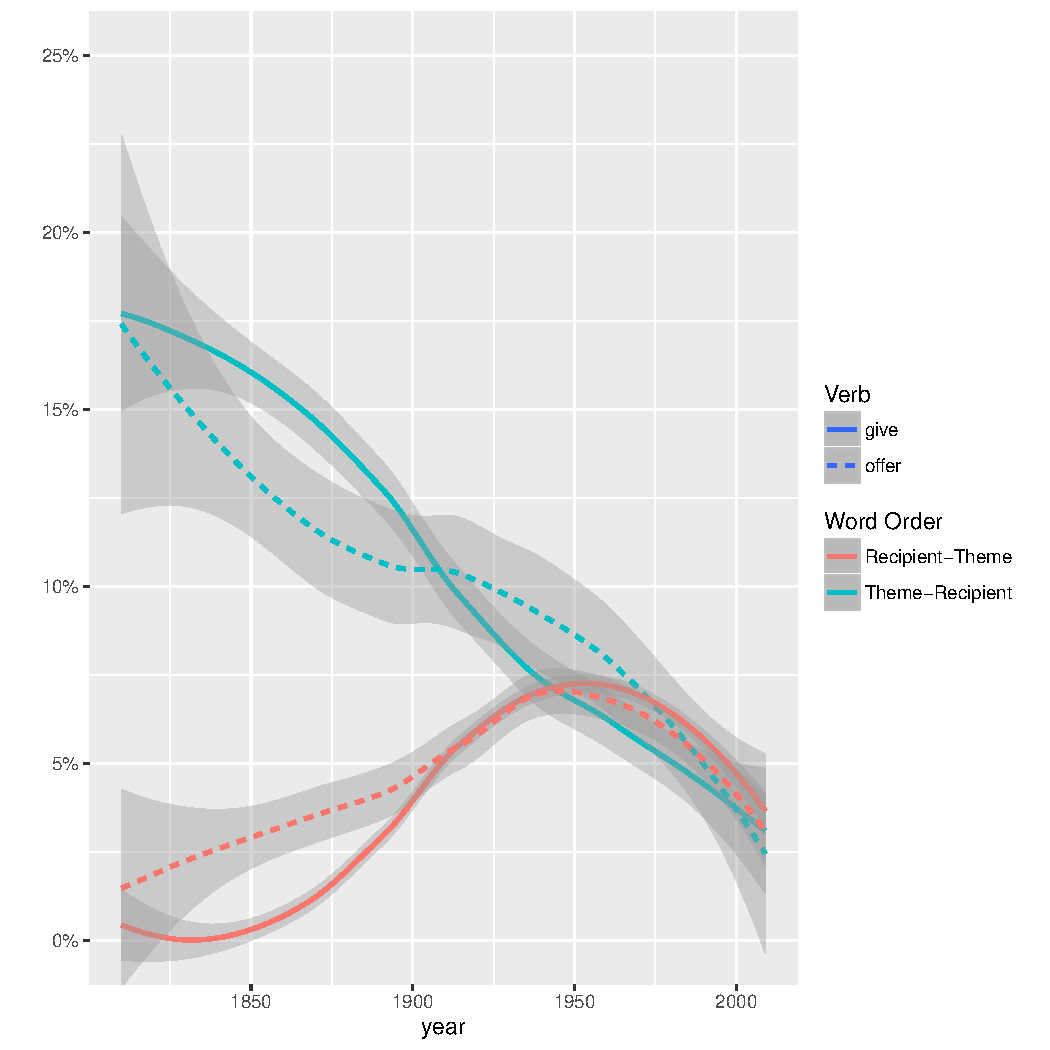
\includegraphics[width=\linewidth]{output/images/am-change-pass}
		\caption{Ditransitive passivisation for GIVE and OFFER from COHA and overall passivisation rate}
		\label{fig:am-change-pass}
	\end{figure}

	I do not have a clear explanation of what formal property changed to produce the change in usage rates in American English. Whatever that formal property is, it specifically targeted the passivisation from underlyingly RT word orders. Throughout Middle and Early Modern English passivisation from underlyingly RT word orders seems marginal in the corpus data (i.e., the usage rates are very low). In 19th century American English, the rate of passivisation in all constructions that are proposed to derive from underlyingly RT word orders in this dissertation increase in usage at the same time. The analysis proposed here (that direct theme passivisation comes from an underlyingly RT word order) is supported by the fact that the two constructions share a shared property under this analysis and the two constructions show parallel development in usage.


\section{Conclusions}
	In this chapter, I showed examples of using quantitative studies in syntactic change to inform linguistic research. This was embedded in a discussion of the nature of linguistic architecture and the relevance of different types of linguistic evidence. Examples were brought to show that quantitative use data can be informative about grammar, but is essential in studying systematic non-grammatical aspects of language.
	
	Looking at the development of recipient marking in English (i.e., the innovation of \textit{to} as the marker of recipients) provided an example of how even complex changes involving the interaction of two distinct changes can be broken apart using relatively simple statistical processes. By breaking apart interacting changes, it is possible to use quantitative measures (such as the Constant Rate Effect) to study the grammatical architecture underlying each change. The quantitative data demonstrated a difference between full noun phrase recipients and pronoun recipients. Within each class, a Constant Rate Effect was found between TR and RT clauses, which supported the uniform analysis of \textit{to} given in this dissertation. However, different slopes were detected between clauses with pronominal recipients and full noun phrase recipients. On the basis of this evidence, I provided an analysis in which pronouns and full noun phrases have different realisations for the recipient P head. While morphological differences between nouns and pronouns are not surprising, given the already known differences between nouns and pronouns in English morphology, this particular difference could not have been discovered without looking at quantitative data.
	
	Looking at recipient passivisation, another case of a clear grammatical change was identified. In particular, both nominative recipient passivisation and pseudopassivisation increase in use during the same time period (Middle and Early Modern English). In this case, there was insufficient data to get strong quantitative results, but the data was consistent with the notion that both nominative recipient passivisation and pseudopassivisation are driven by the same mechanism under this analysis.

	Both of the case studies above show how diachronic syntactic studies can provide independent evidence to support claims made on the basis of synchronic data. In the previous two chapters, I posited two grammatical theories on the basis of synchronic and comparative data: (i) the allomorphy account of dative shift and (ii) the P-incorporation account of nominative recipient passivisation. These grammatical theories made \textit{testable} predictions about diachronic change, in particular predicting Constant Rate Effects. The use of parsed historical corpora provide quantitative data that allows these predictions to be tested. Since the historical data is of a completely different type from the synchronic data (production instead of comprehension; usage rates instead of acceptability judgements), the fact that the synchronic theories predict the diachronic results provides strong independent support to the plausibility of the underlying theories.

	Finally, the rates of recipient passivisation and direct theme passivisation changed together in American English. While there is not clear formal explanation for the change in usage rates, the fact that the use of these two constructions changed in parallel suggests that they share some underlying property (i.e., the property that the change is targeting). I argued that the shared property was passivisation from an underlying RT word order, and used the American English change as another piece of evidence for the analysis of direct theme passivisation as movement of the theme to subject position from an underlying RT word order.

	All of the cases discussed in this chapter shared the property that evidence for particular grammatical analyses was derived from data about the rate at which various grammatical options were used in particular corpora. The underlying logic behind all of these arguments is that concomitant changes in usage reflect a change targeting a particular linguistic property. When two constructions change in parallel, that provides evidence that some change is targeting something shared between the two constructions. By building up a set of constructions that must share \textbf{some} property, it constrains the grammatical analyses to posit some shared property between the different constructions.

%\bibliography{diss}

%\part{Conclusions and Further Implications}\label{part:form}
\chapter{Conclusions and Further Implications}
\section{Conclusions}
This dissertation argued for the dative PP + applicative analysis for recipient ditransitives. Recipient dative PPs were distinguished from goal PPs in so far as goal PPs are merged as the complement of V and recipients are merged in the specifier of an applicative head. Data from typology, focus sensitivity, reconstruction effects, and control possibilities (into purpose clauses) were used to support the notion that the recipient starts off in a position outside of the VP, which C-commands the base position of the theme. After linearisation, this generates a base RT word order in the active.

TR (theme--recipient) word orders were derived by VP-internal scrambling of the theme to a second specifier of the applicative phrase. Focus sensitivity evidence from German as well as scope reconstruction effects from German and English support this analysis. The availability of this operation was subject to variation; Modern Icelandic does not have this operation and only has RT (recipient--theme) word orders in the active. 

Dative shift, where the recipient is marked with a preposition in the TR order and unmarked in the RT order, is attributed to allmorphy in the realisation of the dative P head. Evidence from modern Dutch, quantitative historical evidence from Middle English, and data from High German dialects supports the notion that the P-head that marks recipients in dative shift languages is parallel to the synthetic dative case in languages that have synthetic dative case. For dative shift, the overt allomorph (English \textit{to}) is the default realisation, which is blocked by a null allomorph when the P-head is linearly adjacent to the verb.

This linear adjacency property was sensitive to prior copies of the theme (e.g., ``John gave \sout{the book that he loves} *(to) Mary the book that he loves). This data point granted insight into the ordering of morphological processes, namely that checking linear adjacency for allomorphy must occur before (at least some) copies are deleted.

Considering passive data, Swedish provided overt evidence for the idea that P-incorporation licenses recipient passivisation, since only verbs with overt prefixes (argued to be the reflex of incorporated dative P) allow recipient passivisation. Following \cite{Alexiadou.2014}, Dutch and German were also used to provide evidence in the form of auxiliary variation in the availability of recipient passivisation. The difference between auxiliary variation in OV and prefix vs. non-prefixed verbs in VO languages was used to explore the nature of P-incorporation. This sensitivity to object order provided tangential evidence in favour of a roll-up analysis of object--verb ordering. P-incorporation always moved out of the PP into the next highest functional head; for OV, the next highest head is the auxiliary (after rollup), while, for VO, it is the main verb. This analysis was also supported with quantitative historical English data, where nominative recipient passivisation and pseudopassivisation were found to enter the language in parallel.

Theme passivisation, which is a violation of locality without further syntactic operations (since the recipient intervenes between T and the theme in base generated position), provided evidence for a number of distinct licensing operations. VP-internal scrambling solved the locality problem by moving the theme over the recipient. Recipient cliticisation solved the problem by moving the recipient out of the way of the theme.

When the neither the theme nor the recipient moved, languages varied as to how they solved the locality violation. Most languages only allowed DPs to move to subject position (Icelandic exceptionally allowing dative PPs in subject position). Assuming that PPs were not a valid target for movement, languages treated the intervention differently. For some languages (i.e., some English dialects, Icelandic, German and Dutch), T was able to consider multiple arguments, allowing it to see the theme and to directly move the theme directly to spec-TP. In other languages (e.g., modern American English, Danish and Swedish), T could only consider the highest argument, which caused passivisation to fail, requiring one of the previously mentioned licensing techniques.

\section{Implications}
The conclusions discussed above were only able to be supported by combining data from multiple languages. One clear example of this phenomenon was the typological argument for the RT base order (namely that all Germanic languages have the RT order, but Icelandic lacks the TR order). This type of argument is only possible because a wide variety of languages were surveyed.

Another example is the evidence for P-incorporation. Here Swedish, with its surface realisation of incorporated P-heads, provided the clearest evidence in favour of P-incorporation. However, the same complicated data that makes Swedish ideal for studying P-incorporation makes it a less than ideal case study for arguing for the morphological underpinnings of dative shift. Having access to data from a variety of different languages enabled using the clearest supporting evidence for each point being made, which would have been impossible if only data from one language was used.

Also, diachronic data provided independent support for the analysis. While synchronic evidence from scopal ambiguities and control into purpose clauses is strongly suggestive of the dative PP + applicative analysis, the quantitative analysis of how dative shift developed in the Middle and Early Modern English periods provided a distinct type of evidence that the dative PP + applicative analysis must have been true at an earlier stage of English. Since it was true at an earlier stage, and the modern data is still compatible with the analysis, the most parsimonious explanation is to maintain the analysis throughout the history of English.

The history of recipient passivisation in English provided an example of the interplay between the grammar and performance in cases of variation. With ditransitives, the grammar has a number of different mechanisms for generating grammatical passives (recipient passives and a number of distinct types of theme passives). In some cases (as with nominative recipient passivisation), the necessary mechanism may be commonly used outside of ditransitive passivisation (in this case in pseudopassives). However, the availability of the mechanism in the grammar proves insufficient to generate frequent use of the mechanism in production. For most of modern British English, recipient passivisation was grammatical, but strongly dispreferred. This suggests a two-tiered status of operations within the category of grammatical operations: (a) last-resort operations (grammatical, but only used when necessary) and (b) free-use operations (grammatical and not dispreferred).

The stability through the history of English is a sub-case of the stronger point argued for here. I showed that the dative PP + applicative analysis was compatible with synchronic and diachronic data from all of the major Germanic languages. I proposed that this provides tentative support for the strong UTAH hypothesis \citep{Baker.1988}, namely that \textbf{all} languages share a universal argument structure. In other words, languages cannot vary the base generation positions assigned to arguments. This conclusion resembles the claims about the deep structure of earlier generative traditions \citep{Chomsky.1965,Chomsky.1981}, i.e., that syntax is fundamentally about performing transformations on a universal (possibly non-linguistic) basic structure. This hypothesis is quite falsifiable, in so far as it predicts that the dative PP + applicative analysis should be able to account for recipient data from all natural languages.

A final larger point that this dissertation highlights is the advantage of modularity in approaching linguistic complexity. The Germanic languages showed a large degree of surface variation in the position and surface marking of recipient arguments across active and passive sentences. By distributing the burden of accounting for the surface complexity to the interaction of syntactic and morphological processes, a globally parsimonious account was achieved.

The clearest example of this is the analysis of dative shift. Empirically, dative shift is characterised by an unmarked recipient when adjacent to the verb and a marked recipient elsewhere (with a small number of categoriseable surface exceptions). A purely syntactic approach would need to account for how the syntax is able to identify the linear adjacency of two elements as well as accounting for the difference between marked and unmarked recipients. By using modularity, the syntax of dative shift languages can be made identical to that of non-dative shift languages, with only the addition of the allmorphy operation, which is independently necessary and independently known to be sensitive to linear adjacency. Only because the variation could be attributed to the morphology was the strong UTAH claim explained above possible; languages might have widely varying surface structures that reflect morphological obfuscation of a unified syntactic underpinning.

%\bibliography{diss}

\appendix
\chapter{Statistical Details}
\label{app:stats}

All of the scripts used to collate the data from the parsed corpora and to generate the statistics, tables and figures in the main body of the document can be found at:\\ http://www.github.com/bacovcin/dissertation in the folder called ``analysis''.

\chapter{Germanic Ditansitive Examples}
This appendix collates all of the examples from the main body of the text by language. At the beginning of each language section, I also list all of the works that I referenced to learn about the behaviour of recipient ditransitives in that language. There are details for each of the languages that did not make it into the broader focus of this dissertation. I urge the reader who is interested in the details of a particular language to consult the listed references.

Languages are grouped by language sub-family: North Germanic (Icelandic, Faroese, Norwegian, Swedish and Danish) and then West Germanic (High German, Yiddish, Dutch, Afrikaans, Frisian, Low German and English).

\section{North Germanic}
\subsection{Icelandic}
\subsubsection{Relevant Citations}
\cite{Haugen.1982,Zaenen.1985,Yip.1987,Falk.1990,Maling.1990,Rognvaldsson.1991,Ottosson.1991,Mrck.1992,Ottosson.1993,Kristoffersen.1994,Sprouse.1995,Holmberg.1995,Rognvaldsson.1996,Bardal.1997,Haugen.1998,Holmberg.1998,Maling.1998,Maling.2001,Holmberg.2002,Eythorsson.2005,Bardal.2000,Faarlund.2001,Bardal.2001,Bardal.2001b,Askedal.2001,Dehe.2004,Bardal.2006,Bardal.2007,Thrainsson.2007,Jonsson.2009b,Wallenberg.2011,Norris.2012,Eyorsson.2012,Sigursson.2012,Sigursson.2012b,Alexiadou.2013,Arnadottir.2013,Lundquist.2013,Lundquist.2013b,Alexiadou.2014}
\subsubsection{Active Data}
\begin{exe}
	\exr{ex:ice-rt} Icelandic:
		\gll P\'{e}tur gaf konunginum amb\'{a}ttina.\\
		Peter.NOM gave king.DEF.DAT maid-servant.DEF.ACC.\\
		\trans `Peter gave the king the maid-servant.'

	\exr{ex:ice-tr} Icelandic:
		\gll ?*Hann gaf amb\'attina konunginum.\\
		He.NOM gave maid-servant.DEF.ACC king.DEF.DAT. \\
		\trans `He gave the king the maid-servant \citep[ex 14b]{Dehe.2004}.'
	\exr{ex:icelandic-goals} Icelandic \citep{Thrainsson.2007}:
		\begin{xlist}
		\ex \gll \'{E}g gaf b\ae kurnar til H\'ask\'olab\'okasafnsins\\
		I.NOM gave books.the.ACC to University.Library.the.GEN\\
		\trans `I gave the books to the University Library'
		\ex \gll \th eir seldu skipi\dh  til Englands\\
		they.NOM sold ship.the.ACC to England.GEN\\
		\trans `They sold the ship to England.'
		\end{xlist}

\end{exe}
\subsubsection{Passive Data}
\begin{exe}
	\exr{ex:ice-topic} Icelandic, Topicalization:
\begin{xlist}
	\ex \gll Refinn skaut \textbf{Ólafur} með  þessari byssu.\\
	fox.DEF.ACC shot \textbf{Olaf.NOM} with this shotgun\\
\trans `The fox, Olaf shot with this shotgun \citep[ex. 19a]{Zaenen.1985}.'
\ex[*]{\gll Með  þessari byssu skaut \textbf{refinn} Ólafur.\\
	with this shotgun shot \textbf{fox.DEF.ACC} Olaf.NOM\\
\trans `The fox, Olaf shot with this shotgun \citep[ex. 19b]{Zaenen.1985}.'}
\end{xlist}
\exr{ex:ice-dq} Icelandic, Direct Question:
\begin{xlist}
	\ex \gll Hafði \textbf{Sigga} aldrei hjálpað Haraldi?\\
	had \textbf{Sigga.NOM} never helped Harald.DAT\\
\trans `Had Sigga never helped Harald \citep[ex. 20b]{Zaenen.1985}?'
\ex[*]{\gll Hafði \textbf{Haraldi} Sigga aldrei hjálpað?\\
	had \textbf{Harald.DAT} Sigga.NOM never helped\\
\trans `Had Sigga never helped Harald \citep[ex. 20c]{Zaenen.1985}?'}
\end{xlist}
	\exr{ex:ice-dittop} Icelandic, Ditransitive Topicalization:
\begin{xlist}
	\ex \gll Um veturinn voru \textbf{konunginum} gefnar amb\'{a}ttir.\\
In winter.the were \textbf{king.the.DAT} given slaves.NOM\\
\trans `In the winter the king was given slaves \citep[ex. 47a]{Zaenen.1985}.'
\end{xlist}
\exr{ex:ice-ditdq} Icelandic, Ditransitive Direct Question:
\begin{xlist}
	\ex \gll Voru \textbf{konunginum} gefnar amb\'{a}ttir?\\
were \textbf{king.the.DAT} given slaves.NOM\\
\trans `Was the king given slaves \citep[ex. 48a]{Zaenen.1985}?'
\end{xlist}


	\exr{ex:ice-directthe} Icelandic:
	\begin{xlist}
		\ex \gll Um veturinn voru \textbf{amb\'{a}ttin} gefin konunginum \sout{amb\'{a}ttin}.\\
		In winter.the was \textbf{slave-the.NOM} given king.the.DAT \sout{slave-the.NOM}\\
		\trans `In the winter the slave was given to the king \citep[ex. 47b]{Zaenen.1985}.'
		\ex \gll Var \textbf{amb\'{a}ttin} gefnar konunginum \sout{amb\'{a}ttin}?\\
		were \textbf{slave-the.NOM} given king.the.DAT \sout{slave-the.NOM}\\
		\trans `Was the slave given to the king \citep[ex. 48b]{Zaenen.1985}?'
		\ex \gll \textbf{B\'{o}kin} var gefin J\'{o}ni \sout{B\'{o}kin}\\
		\textbf{book-the.NOM} was given John.DAT \sout{book-the.NOM}\\
		\trans `The book was given to John \citep{Holmberg.1995,Bardal.2001}.'
	\end{xlist}

	\exr{ex:ice-ppsbj} Icelandic:
	\begin{xlist}
		\ex[*]{\gll {\'{I} gar} var um þessa konu oftast talað\\
		yesterday was about this woman often talked\\
		\trans `Yesterday, this woman was often talked about'}
		\ex[*]{\gll {\'{I} gar} var \'{i} r\'{u}minu sofið\\
		yesterday was in bed.DEF slept\\
		\trans `Yesterday, the bed was slept in.'}
	\end{xlist}
\end{exe}

\subsection{Faroese}
\subsubsection{Relevant Citations}
\cite{Haugen.1982,Barnes.1986,Hoskuldurrainsson.2004,Bardal.2007,Jonsson.2009,Eyorsson.2012,Arnadottir.2013,Lundquist.2013,Lundquist.2013b}
\subsubsection{Active Data}
\begin{exe}
	\exr{ex:far-rt} Faroese:
		\gll Hon gav Mariu troyggiuna.\\
		She gave Maria.DAT sweater.DEF.ACC.\\
		\trans `She gave Maria the sweater \citep{Lundquist.2013b}.'
	\exr{ex:far-tr}[\%]{Faroese:
		\gll Hon gav telduna til gentuna.\\
		she gave computer-the.ACC to girl-the.ACC\\
		\trans `She gave the computer to the girl.'}
	\exr{ex:far-case} Faroese:
		\begin{xlist}
			\ex[ ]{\gll Teir góvu \textbf{gentuni} telduna \\
				they gave \textbf{girl-the.DAT} computer-the.ACC \\
			            \trans `They gave the girl the computer.'}
				    \ex[*]{\gll Teir góvu \textbf{gentuna} telduna \\
				they gave \textbf{girl-the.ACC} computer-the.ACC \\
			    \trans `They gave the girl the computer.'}
		\end{xlist}

\end{exe}
\pagebreak
\subsubsection{Passive Data}
\begin{exe}
		\exr{ex:far-pass} Faroese:
		\begin{xlist}
		\ex[ ]{\gll Gentan bleiv givin telduna\\
			    girl-the.NOM was given.NOM computer-the.ACC\\
		    	    \trans `The girl was given the computer.'}
		\ex[??]{\gll Gentuni bleiv givin ein telda\\
			    girl-the.DAT was givn.NOM a.NOM computer.NOM\\
		    	    \trans `The girl was given the computer.'}
		\end{xlist}
\end{exe}

\subsection{Norwegian}
\subsubsection{Relevant Citations}
\cite{Haugen.1982,Afarli.1992,Sprouse.1995,Holmberg.1995,Kristoffersen.1994,Askedal.2001,Holmberg.2002,Bardal.2007,Kinn.2010,Afarli.2012,Eyorsson.2012,Lundquist.2013,Lundquist.2013b,Haddican.2014}
\subsubsection{Active Data}
\begin{exe}
	\exr{ex:nor-rt} Standard Norwegian:
		\gll Jeg har gitt mannen boken.\\
		I have given man.DEF book.DEF.\\
		\trans `I gave the man the book \citep[ex 10]{Sprouse.1995}.'

	\exr{ex:nor-tr} Norwegian:
		\gll Vi har lånt den interessante boken du nevnte *(til) Petter.\\
		we have lent the interesting book you mentioned to Peter.\\
		\trans `We have lent the interesting book you mentioned to Peter \citep{Larson.1988}.'
	\exr{ex:halsa-case} Halsa Norwegian:
	\begin{xlist}
		\ex \gll Ho erta \textbf{katt\aa} \\
		she teased \textbf{cat.DEF.ACC} \\
			\trans `She teased the cat.'
			\ex \gll Ho ga \textbf{katt\aa inn} mat \\
			she gave \textbf{cat.DEF.DAT} food \\
			\trans `She gave the cat food.'
	\end{xlist}
	
\end{exe}
\subsubsection{Passive Data}
\begin{exe}
	\exr{ex:nor-null-incorp} Standard Norwegian:
		\gll Han vart P=$\emptyset$-gitt \sout{hann} ein medalje\\
		he.NOM was given \sout{he.NOM} a medal\\
		\trans `He was given a medal.'
	\exr{ex:halsa-pass} Halsa Norwegian:
	\begin{xlist}
		\ex[ ]{\gll Hainn vart gjevinn ei skei.\\
		He.NOM was given a spoon\\
		\trans `He was given a spoon.' \cite[ex 50c]{Eyorsson.2012}}
		\ex[*]{\gll Hånnå vart gjevinn ei skei.\\
		He.DAT was given a spoon\\
		\trans `He was given a spoon.' \cite[ex 50c]{Eyorsson.2012}}
	\end{xlist}
\end{exe}
\subsection{Swedish}
\subsubsection{Relevant Citations}
\cite{Haugen.1982,Falk.1990,Falk.1993,Holmberg.1995,Falk.1997,Anward.1989,Holmberg.2002,Lundquist.2004,Platzack.2005,Lundquist.2006,Bardal.2007,Lundquist.2013,Lundquist.2013b,Haddican.2014,Haddican.2015}
\subsubsection{Active Data}
\begin{exe}
	\exr{ex:sw-rt} Swedish:
		\gll Jag gav Johan en bok.\\
		I gave John a book.\\
		\trans `I gave John a book \citep{Holmberg.1995}.'
	\pagebreak
	\exr{ex:sw-tr} Swedish:
		\gll Jag gav en bok *(til) Johan.\\
		I gave a book to John.\\
		\trans `I gave a book to John \citep{Holmberg.1995}.'

	\exr{ex:sw-act-simple} Swedish:
			\begin{xlist}
				\ex \gll Han gav Jan bollen\\
				he.NOM gave John ball.the\\
				\trans `He gave John the ball'
				\ex \gll Han gav bollen *(til) Jan\\
				he.NOM gave ball.the to John\\
				\trans `He gave the ball to John'
			\end{xlist}
	\exr{ex:Swedish-complex-act} Swedish:
			\begin{xlist}
				\ex[ ]{\gll Han erbjöd Jan ett nytt jobb\\
				he.NOM offered John a new job\\
			\trans `He offered John a new job'}
				\ex[??]{\gll Han erbjöd ett nytt jobb til Jan\\
				he.NOM offered a new job to John\\
			\trans `He offered a new job to John'}
				\ex[*]{\gll Han erbjöd ett nytt jobb Jan\\
				he.NOM offered a new job John\\
			\trans `He offered a new job to John'}
			\end{xlist}

\end{exe}
\subsubsection{Passive Data}
\begin{exe}
	\exr{ex:swe-part} Swedish:
	\begin{xlist}
		\ex[ ]{Particle Verb:
		\gll Han erbjöds ett nytt jobb\\
			he.NOM offered.PASS a new job\\
			\trans `He was offered a new job (\citealt{Anward.1989}, \citealt{Lundquist.2006}).'}
		\pagebreak
		\ex[*]{Non-Particle Verb:
		\gll Pelle gavs ett äpple\\
			Pelle gave.PASS a apple\\
			\trans `Pelle was given an apple (\citealt{Anward.1989}, \citealt{Lundquist.2006}).'}
	\end{xlist}	
	\exr{ex:swe-nopart-pass} Swedish (verbs without particles):
		\sn[*]{
			\gll Ett äpple gavs Pelle.\\
			 An apple gave.PASS Pelle.\\
			 \trans `An apple was given to Pelle (\citealt{Anward.1989},\citealt{Lundquist.2006}).'}
	\exr{ex:sw-offer-pass} Swedish:
		\gll Ett nytt jobb erbjöds=honom.\\
		A new job offered.PASS=him.OBL.\\
		\trans `A new job was offered to him (\citealt{Anward.1989},\citealt{Falk.1990},\citealt{Lundquist.2006}).'
	\exr{ex:sw-give-pass} Swedish:
		\gll *Ett äpple gavs honom.\\
		 An apple gave.PASS him.\\
		 \trans `An apple was given to him (\citealt{Anward.1989},\citealt{Lundquist.2006}).'
	 \exr{ex:sw-offer-thepas} Swedish:
		\gll Jobbet erbjöds mannen med den långa svarta kappan.\\
		job.DEF offered.PASS man.DEF with the long black coat\\
		'The job was offered to the man with the long black coat \citep[ex 26]{Lundquist.2004}.'

	\exr{ex:sw-relpass} Swedish:
		\begin{xlist}
			\ex[ ]{\gll \textbf{DET} \textbf{jobbet} har Kalle tilldelats.\\
			that job.DEF has Kalle assigned.PART.PASS\\
			\trans `THAT job, Kalle has been assigned \citep[ex. 59]{Lundquist.2004}.'}
			\ex[??]{\gll DEN mannen har jobbet tilldelats.\\
			that man.DEF has job.DEF assigned.PART.PASS\\
			\trans `To THAT man, the job has been assigned \citep[ex. 58]{Lundquist.2004}.'}
		\end{xlist}
		\pagebreak
	\exr{ex:sw-relpass2} Swedish:
		\begin{xlist}
			\ex[ ]{\gll Jobbet som erbjöds \textbf{mannen} var mycket slitsamt.\\
			job.DEF which offered.PASS \textbf{man.DEF} was very tiring\\
			\trans `The job, which was offered to the man, was very tiring \citep[ex. 49]{Lundquist.2004}.'}
			\ex[ ]{\gll Jobbet som \textbf{mannen} erbjöds var mycket slitsamt.\\
			job.DEF which \textbf{man.DEF} offered.PASS was very tiring\\
			\trans `The job, which the man was offered, was very tiring \citep[ex. 50]{Lundquist.2004}.'}
		\end{xlist}
\end{exe}



\subsection{Danish}
\subsubsection{Relevant Citations}
\cite{Haugen.1982,Herslund.1986,Vikner.1989,Falk.1990,Sprouse.1995,Allan.1995,Bardal.2007,Lundquist.2013,Lundquist.2013b}
\subsubsection{Active Data}
\begin{exe}
	\exr{ex:dan-rt} Danish:
		\gll Peter viste jo Marie bogen.\\
		Peter showed indeed Mary book.DEF.\\
		\trans `Peter indeed showed Mary the book \citep{Vikner.1989}.'
	\exr{ex:dan-tr} Danish:
		\gll Jeg gav bogen *(til) Anna.\\
		I gave book.the to Anna.\\
		\trans `I gave the book to Anna\citep{Holmberg.1998}.'
\end{exe}
\subsubsection{Passive Data}
\begin{exe}
	\exr{ex:dan-pass} Danish:
	 \sn[*]{
	 \gll En stilling blev tilbudt ham.\\
A job was offered him.OBL.\\
\trans `A job was offered to him \citep{Falk.1990}.'}

	\exr{ex:dan-null-incorp} Danish:
	\gll Han blev P=$\emptyset$-tilbudt \sout{hann} en stilling\\
	he.NOM was offered \sout{he.NOM} a job\\
	\trans `He was offered a job.'
	\exr{ex:dan-pseudopass} Danish:
	\begin{xlist}
		\ex[ ]{\gll Revisionen blev \textbf{p\aa begyndt} i maj\\
		revision-the was \textbf{on-begun} in May\\
		\trans `The revision was begun in May'}
		\ex[*]{\gll Revisionen blev \textbf{begyndt} \textbf{p\aa} i maj\\
		revision-the was \textbf{begun} \textbf{on} in May\\
		\trans `The revision was begun in May'}
	\end{xlist}
\end{exe}




\section{West Germanic}
\subsection{High German}

\subsubsection{Relevant Citations}
\cite{Shrier.1965,Lenerz.1977,Werner.1982,Hohle.1982,Webelhuth.1984,Scherpenisse.1986,Abraham.1986,Webelhuth.1989,Besten.1990,Czepluch.1990,Frey.1993,Lee.1994,Sprouse.1995,Draye.1996,Leirbukt.1997,Holmberg.1998,McGinnis.1998,Maling.2001,Frey.2001,Seiler.2001,Askedal.2001,Bayer.2001,Seiler.2003,McFadden.2004,Platzack.2005,McFadden.2006,Meinunger.2006,Eythorsson.2005,Bardal.2006,Fleischer.2006,Georgala.2011,Georgala.2011b,Alexiadou.2013b,Alexiadou.2014}
\subsubsection{Active Data}
\begin{exe}
	\exr{ex:german-forms} High German, Dative--Preposition Alternation:
	\begin{xlist}
		\ex  \gll Ich habe der Frau das Buch geschickt\\
			I.NOM have the.DAT woman the.ACC book sent\\
			 \trans `I sent the woman the book.'
		 \ex \gll Ich habe das Buch der Frau geschickt\\
			 I.NOM have the.ACC book the.DAT woman sent\\
			 \trans `I sent the woman the book.'
		 \ex \gll Ich habe das Buch an die Frau geschickt\\
			 I.NOM have the.ACC book to the.ACC woman sent\\
			 \trans `I sent the book to the woman.'
	\end{xlist}
	\exr{ex:hg-rt} High German:
		\gll weil er der Unehrlichkeit keine Chance gibt.\\
		as he.NOM the.DAT dishonesty no.ACC opportunity gives.\\
		\trans `as he gives dishonesty no opportunity \citep[162]{Draye.1996}.'
	\exr{ex:hg-tr} High German:
		\gll weil er keine Chance der Unehrlichkeit gibt.\\
		as he.NOM no.ACC opportunity the.DAT dishonesty gives.\\
		\trans `as he gives no opportunity to dishonesty'
	\exr{ex:german-goals} High German:
		\begin{xlist}
			\ex[\#]{\gll Er hat \textbf{Maria} einen Brief geschickt, aber er ist bei ihr nicht angekommen\\
			he.NOM has \textbf{Maria} a.ACC letter sent, but he.NOM is by her.DAT not arrived\\
			\trans `He sent Maria a letter, but it has not reached her.'}
			\ex[\#]{\gll Er hat einen Brief \textbf{Maria} geschickt, aber er ist bei ihr nicht angekommen\\
			he.NOM has a.ACC letter \textbf{Maria} sent, but he.NOM is by her.DAT not arrived\\
			\trans `He sent a letter to Maria, but it has not reached her.'}
			\ex[ ]{\gll Er hat einen Brief \textbf{an} \textbf{Maria}  geschickt, aber er ist bei ihr nicht angekommen\\
			he.NOM has a.ACC letter \textbf{to} \textbf{Maria} sent, but he.NOM is by her.DAT not arrived\\
			\trans `He sent a letter to Maria, but it has not reached her.'}
		\end{xlist}
		\pagebreak
	\exr{ex:german-VP-top} High German, VP-topicalisation:
		\begin{xlist}
			\ex \gll  Dem Mann das Buch gegeben habe ich, (nicht der Frau dEN Film geschenkt).\\
			the.DAT man the.ACC book given have I, (not the.DAT woman the.ACC film sent).\\
			\trans `It was giving the man the book that I did (not sending the woman the film).'
			\ex \gll Das Buch dem Mann gegeben habe ich, (nicht dEN Film der Frau geschenkt).\\
			the.ACC book the.DAT man given have I, (not the.ACC film the.DAT woman sent).\\
			\trans `It was giving the book to the man that I did (not sending the film to the woman).\\
		\end{xlist}
	\exr{ex:hg-vp-top-goals} High German, VP-topicalisation:
		\begin{xlist}
			\ex[*]{ \gll  An den Mann das Buch geschickt habe ich, (nicht an die Frau dEN Film übergeben).\\
			to the.ACC man the.ACC book sent have I, (not to the.ACC woman the.ACC film delivered).\\
		\trans `It was sending to the man the book that I did (not delivering to the woman the film).'}
		\ex[ ]{\gll Das Buch an den Mann gegeben habe ich, (nicht dEN Film an die Frau übergeben).\\
			the.ACC book to the.ACC man given have I, (not the.ACC film to the.ACC woman delivered).\\
		\trans `It was sending the book to the man that I did (not delivering the film to the woman).\\}
	\end{xlist}

	\exr{ex:hg-rec-focus} High German, Recipient Focus \citep{Choi.1996}:
		\gll Wem hast du das Geld gegeben?\\
		whom.DAT have you.NOM the money.ACC given\\
		\trans `Who did you give the money to?'
		\begin{xlist}
			\ex \gll Ich habe dem KASSIERER das Geld gegeben.\\
			I.NOM have the cashier.DAT the money.ACC given.\\
			\trans `I have given the cashier the money.'
			\ex \gll Ich habe das Geld dem KASSIERER gegeben.\\
			I.NOM have the money.ACC the cashier.DAT given.\\
			\trans `I have given the money to the cashier.'
		\end{xlist}
	\exr{ex:hg-theme-focus} High German, Theme Focus \citep{Choi.1996}:
		\gll Was hast du dem Kassierer gegeben?\\
		what.ACC have you.NOM the cashier.DAT given\\
		\trans `What did you give to the cashier?'
		\begin{xlist}
			\ex[ ]{\gll Ich habe dem Kassierer das GELD gegeben.\\
			I.NOM have the cashier.DAT the money.ACC given.\\
			\trans `I have given the cashier the money.'}
			\ex[?*]{\gll Ich habe das GELD dem Kassierer gegeben.\\
			I.NOM have the money.ACC the cashier.DAT given.\\
			\trans `I have given the money to the cashier.'}
		\end{xlist}
	\exr{ex:hg-binding-rt} High German, recipient--theme:
		\begin{xlist}
			\ex[ ]{\gll dass Maria jedem seinen Nachbarn vorgestellt hat.\\
			that Maria everyone.DAT his.ACC neighbour.ACC introduced has.\\
			\trans `that Maria introduced everyone his neighbor \citep[ex. 11a]{Lee.1994}.'}
			\ex[*]{\gll dass Maria seinem Nachbarn jeden vorgestellt hat.\\
			that Maria his.DAT neighbour.DAT everyone.ACC introduced had.\\
			\trans `that Maria introduced everyone to his neighbour \citep[ex. 9a]{Lee.1994}.'}
		\end{xlist}
	\exr{ex:hg-binding-tr} High German, theme--recipient:
		\begin{xlist}
			\ex[ ]{\gll dass Maria jeden seinem Nachbarn vorgestellt hat.\\
			that Maria everyone.ACC his.DAT neighbour.DAT introduced had.\\
			\trans `that Maria introduced everyone to his neighbour \citep[ex. 10a]{Lee.1994}.'}
			\ex[\%]{\gll dass Maria seinen Nachbarn jedem vorgestellt hat.\\
			that Maria his.ACC neighbour.ACC everyone.DAT introduced had.\\
			\trans `that Maria introduced everyone his neighbour \citep[ex. 12a (note 10)]{Lee.1994}.'}
		\end{xlist}


	\exr{ex:hg-creation} High German \citep[ex 31]{Frey.2001}:
	\begin{xlist}
		\ex[ ]{\gll dass Hans geschickt eine Flöte schnitzte\\
		that John skillfully a.ACC flute carved\\
		\trans `that John skillfully carved a flute.'}
		\ex[*]{\gll dass Hans eine Flöte geschickt schnitzte\\
		that John a.ACC flute skillfully carved\\
		\trans `that John skillfully carve a flute.'}
	\end{xlist}
	\exr{ex:hg-VPadverb} High German, VP-level adverbs:
		\begin{xlist}
			\ex \gll Ich habe nicht dem Mann das Buch gegeben, SONDERN DER FRAU DEN FILM GESCHENKT.\\
			I have not the.DAT man the.ACC book given, but the.DAT woman the.ACC film sent.\\
			\trans `I didn't give the man the book, instead I sent the woman the film.'
			\ex \gll Ich habe nicht das Buch dem Mann gegeben, SONDERN DEN FILM DER FRAU GESCHENKT.\\
			I have not the.ACC book the.DAT man given, but the.ACC film the.DAT woman sent.\\
			\trans `I didn't give the book to the man, insead I sent the film to the woman.'
		\end{xlist}
	\exr{german-nom} High German, Nominalisation:
		\begin{xlist}
			\ex[ ]{\gll Oswald hat den P\"{a}sident errnordet\\
			Oswald has the president.ACC assassinated\\
			\trans `Oswald assassinated the president \citep[ex 5a]{Bayer.2001}'}
			\ex[ ]{\gll die Ermordung des Pr\"{a}sidenten\\
			the.NOM assassination the.GEN president\\
			\trans `the assassination of the president \citep[ex 5c]{Bayer.2001}'}
			\ex[ ]{\gll Oswald hat dem Pr\"{a}sidenten gehuldigt\\
			Oswald has the.DAT president given-homage\\
			\trans `Oswald gave homage to the president \citep[ex 6a]{Bayer.2001}'}
			\ex[*]{\gll die Huldigung des/dem Pr\"{a}sidenten\\
			the.NOM homage-giving the.GEN/the.DAT president\\
			\trans `the homage giving to the president \citep[ex 6]{Bayer.2001}'}
		\end{xlist}
\pagebreak
	\exr{ex:zurich} Zürich German:
		\gll si schänkt äine \textbf{a} \textbf{de} \textbf{Tristane}\\
		they.NOM sent one.ACC to the Tristan\\
		\trans `The sent one to Tristan \citep[pg. 175]{Seiler.2003}.'
	\exr{ex:luzern} Luzern German:
		\gll miir verchauggid \textbf{i} \textbf{de} \textbf{Chunde} nur Mère-Josephine-Poulets\\
		we.NOM sold to the clients only Mere-Josephine chicken\\
		`We sold the clients only Mere-Josephine chicken \citep[pg. 175]{Seiler.2003}.'
	\exr{ex:hg-Pcomp} High German:
		\begin{xlist}
			\ex \gll in + P$_{goal}$ den Baum\\
				 in + P$_{goal}$ the.ACC tree\\
				 \trans `into the tree'
			\ex \gll in + P$_{location}$ dem Baum\\
				 in + P$_{location}$ the.DAT tree\\
				 \trans `in the tree'
		\end{xlist}

\end{exe}
\subsubsection{Passive Data}
\begin{exe}
	\exr{ex:hg-accnom} High German:
		\begin{xlist}
			\ex \gll Ich habe den Mann gesehen\\
			I.NOM have the.\textbf{ACC} man seen\\
			\trans `I saw the man.'
			\ex \gll Der Mann wurde gesehen\\
			the.\textbf{NOM} man was seen\\
			\trans `The man was seen.'
		\end{xlist}
	\exr{ex:hg-insitu-sbj} High German:
		\gll Ich glaube, dass den Kindern das Fahrrad geschenkt worden ist.\\
		I beleive that the.DAT.PL children the.NOM bicycle granted become be.3sg\\
		\trans `I believe that the child was granted the bicycle.'
	\pagebreak
	\exr{ex:hg-normal-pass} High German:
		\begin{xlist}
			\ex[ ]{\gll Ich glaube, dass \textbf{den} \textbf{Kindern} das Fahrrad geschenkt worden ist.\\
			I beleive that \textbf{the.DAT.PL} \textbf{children} the.NOM bicycle granted become be.3sg\\
			\trans `I believe that the children were granted the bicycle.'}
			\ex[*]{\gll Ich glaube, dass \textbf{die} \textbf{Kindern} das Fahrrad geschenkt worden sind.\\
			I beleive that \textbf{the.NOM.PL} \textbf{children} the.ACC bicycle granted become be.3pl\\
			\trans `I believe that the children were granted the bicycle.'}
		\end{xlist}
	\exr{ex:hg-get-pass} High German:
		\begin{xlist}
			\ex \gll dass der Vater \textbf{der} \textbf{Tochter} ein Buch geschenkt hat\\
			that the.NOM father \textbf{the.DAT} \textbf{daughter} a.ACC book sent has\\
			\trans `that the father sent the daughter a book.'
			\ex \gll dass \textbf{die} \textbf{Tochter} von dem Vater ein Buch geschenkt bekommen hat\\
			that \textbf{the.NOM} \textbf{daughter} by the father a.ACC book sent got has\\
			\trans `that the daughter got sent a book by her father \cite[183]{Draye.1996}.'
		\end{xlist}

\end{exe}
\subsection{Yiddish}
\subsubsection{Relevant Citations}
\cite{Birnbaum.1979,Holmberg.1998}
\subsubsection{Active Data}
\begin{exe}
	\exr{ex:yid-rt} Yiddish:
		\gll Zi git der snjjer dus pékl. \\
		she.NOM gives the.DAT daughter-in-law the.ACC parcel.\\
		\trans 'She gives her daughter-in-law the parcel \citep[ex 190a]{Birnbaum.1979}.'
\end{exe}
\subsubsection{Passive Data}
No examples.


\subsection{Dutch}
\subsubsection{Relevant Citations}
\cite{Scherpenisse.1986,Besten.1990,Hoekstra.1991,SchermerVermeer.1991,Broekhuis.1994,Sprouse.1995,DenDikken.1995,Sprouse.1995,Holmberg.1995,vanBelle.1996b,Holmberg.1998,Holmberg.2002,Anagnostopoulou.2003,Donaldson.2008,Colleman.2009,Colleman.2009b,Colleman.2010,Colleman.2010b,Colleman.2011,Colleman.2010c,Colleman.2012,Broekhuis.2012,Alexiadou.2013b,Alexiadou.2014}
\subsubsection{Active Data}
\begin{exe}
	\exr{ex:dut-rt} Dutch:
		\gll Ik heb (aan) Jan een boek gegeven.\\
		I have (to) Jan a book given.\\
		\trans `I gave Jan a book \citep{Tiersma.1985}.'
	\exr{ex:dut-tr} Dutch:
		\gll Ik heb een boek *(aan) Jan gegeven.\\
		I have a book *(to) Jan given.\\
		\trans `I gave a book to Jan.'
	\exr{ex:dutch-rec-marking} Dutch:
		\begin{xlist}
			\ex \gll Ik heb een boek *(aan) Jan gegeven\\
			I have a book to John given\\
			\trans `I gave a book to John \citep{Tiersma.1985}.'
			\ex \gll Ik heb (aan) Jan een boek gegeven\\
			I have to John a book given\\
			\trans `I gave John a book \citep{Tiersma.1985}.'
		\end{xlist}

\end{exe}
\subsubsection{Passive Data}
\begin{exe}
	\exr{ex:dutch-normal-pass} Dutch:
		\begin{xlist}
			\ex[ ]{\gll De boeken \textbf{werden} haar aangeboden.\\
			the books \textbf{became.PL} her given\\
			\trans `The books were given to her.' \citep[ex. 5b]{Broekhuis.1994}}
			\ex[*]{\gll Zij \textbf{werd} de boeken aangeboden.\\
			she.NOM \textbf{became.SG} the books given\\
			\trans `She was given the books.' \citep[ex. 5c]{Broekhuis.1994}}
		\end{xlist}
	\exr{ex:dut-insitu-sbj} Dutch:
		\gll Er werd mij een boek gegeven.\\
		There became.3sg me a book given\\
		\trans `A book was given to me. \cite[pg 245]{Donaldson.2008}'
	\exr{ex:dut-get-pass} Dutch:
		\gll \textbf{Zij} kreeg de boeken (van mij) aangeboden.\\
		\textbf{she.NOM} got the books (by me) given\\
		\trans `She was given the books (by me).' \citep[ex. 7]{Broekhuis.1994}
	\exr{ex:dut-scram} Dutch:
	\begin{xlist}
		\ex[ ]{\gll dat het boek \textbf{Marie} waarschijnlijk gegeven wordt\\
		that the book \textbf{Mary} probably given was\\
		\trans `that the book was probably given to Mary.'}
		\ex[?*]{\gll dat het boek waarschijnlijk \textbf{Marie} gegeven wordt\\
		that the book probably \textbf{Marie} given was\\
		\trans `that the book was probably given to Mary.'}
	\end{xlist}

\end{exe}

\subsection{Afrikaans}
\subsubsection{Relevant Citations}
\cite{Donaldson.1993,Stadler.1996,Louw.2012}
\subsubsection{Active Data}
\begin{exe}
	\exr{ex:af-rt} Afrikaans:
		\gll dat die man die vrou `n dokument gegee het.\\
		that the man the woman a document given has.\\
		\trans `...that the man gave a document to the woman \citep{Louw.2012}.'
	\exr{ex:af-tr} Afrikaans:
		\gll Ek het `n fooitjie aan hom gegee.\\
		I have a tip to him given.\\
		\trans `I have given a tip to him \citep{Stadler.1996}.'

\end{exe}
\subsubsection{Passive Data}
\begin{exe}
	\exr{ex:af-rec-pass1} Afrikaans: 
		\begin{xlist}
			\ex \gll Is aan hom ooit 'n geskenk gegee?\\
			Was to him ever a present given.\\
			\trans `Was he ever given a present \citep[ex. 49]{Stadler.1996}?'
			\ex \gll Gister is aan hom `n klomp geld gegee.\\
			Yesterday was to him a {lot of} money given.\\
			\trans `Yesterday he was given a lot of money \citep[ex. 50]{Stadler.1996}.'
	\end{xlist}

	\exr{ex:af-rec-pass2} Afrikaans:
		\begin{xlist}
			\ex[?]{\gll hy is `n present gegee.\\
			he was a present given\\
			\trans `He was given a present \citep[ex. 35]{Stadler.1996}.'}
			\ex[ ]{\gll Aan hom is `n present gegee.\\
			to him was a present given\\
			\trans `He was given a present \citep[ex. 44]{Stadler.1996}.'}
		\end{xlist}

\end{exe}


\subsection{Frisian}
\subsubsection{Relevant Citations}
\cite{Tiersma.1985}
\subsubsection{Active Data}
\begin{exe}
	\exr{ex:fri-rt} Frisian:
		\gll se joech jar kammeraatske in skjirre.\\
		she gave her girlfriend a {pair of scissors}.\\
		\trans `She gave her girlfriend a pair of scissors.'

	\exr{ex:fri-tr} Frisian:
		\gll ik joech in plant oan Beppe.\\
		I gave a plant to Grandmother.\\
		\trans `I gave a plant to Grandmother \citep{Tiersma.1985}.'

\end{exe}
\subsubsection{Passive Data}
No examples.

\subsection{Low German}
\subsubsection{Relevant Citations}
\cite{Mussaus.1829,Lasch.1914,Keseling.1970,Ponelis.1979,Ponelis.1993,Boden.1993,Lindow.1998,Appel.2007}
\subsubsection{Active Data}
\begin{exe}
	\exr{ex:lg-rt} Low German:
		\gll ick gaw den Mann dat Brod.\\
		I gave the man the bread.\\
		\trans `I gave the man the bread \citep{Mussaus.1829}.'

	\exr{ex:lg-tr} Low German:
		\gll ick gaw dat Brod den Man, wobei dat Brod zeigend ist.\\
		I gave the bread the man who the bread shown is.\\
		\trans `I gave the bread to the man who was shown the bread \citep{Mussaus.1829}.'
\end{exe}
\subsubsection{Passive Data}
No examples.

\subsection{English}
\subsubsection{Relevant Citations}
\cite{Fillmore.1965,Emonds.1972,Langendoen.1973,Oehrle.1976,Hornstein.1981,McLaughlin.1983,Mitchell.1985,Barss.1986,Larson.1988,Gropen.1989,Anward.1989,Aoun.1989,Maling.1990,Falk.1990,Jackendoff.1990,Johnson.1991,Hoekstra.1991,Levin.1993,DenDikken.1995,Sprouse.1995,Collins.1995,Holmberg.1998,Allen.1999,Kroch.2000,Maling.2001,Bruening.2001,Oba.2002,Polo.2002,McFadden.2002,Harley.2002,Taylor.2003,Anagnostopoulou.2003,McFadden.2004,Kroch.2004,Postal.2004,Platzack.2005,Oba.2005,Alexiadou.2005,Levinson.2005,Taylor.2006,Bresnan.2007,Gast.2007,Hovav.2008,Bresnan.2009,Kroch.2010,Levin.2010,Bresnan.2010,Davies.2010,Bruening.2010,Bruening.2010b,Haddican.2010,Larson.2010,Myler.2011,Haddican.2011,Haddican.2012,Ormazabal.2012,SowkaPietraszewska.2013,Gerwin.2013,Bruening.2014,Haddican.2014,Sigursson.2014,Biggs.2015,Cuypere.2015,Hallman.2015,Harley.2015}
\subsubsection{Active Data}
\begin{exe}
	\exr{ex:eng-rt} English: I gave the man the book.
	\exr{ex:en-tr} English: I gave the book to the man.
	\exr{ex:dat-shift} Modern American English, Dative Shift:
	\begin{xlist}
		\ex I sent the woman the book.
		\ex I sent the book to the woman.
	\end{xlist}
	\pagebreak
	\exr{ex:eng-rec-wh} English, Recipients:
		\begin{xlist}
			\ex[ ]{Who did you give the package to?}
			\ex[*]{Where did you give the package to?}
		\end{xlist}
	\exr{ex:eng-goal-wh} English, Goals:
		\begin{xlist}
			\ex[ ]{Who did you send the package to?}
			\ex[ ]{Where did you send the package to?}
		\end{xlist}
	\exr{ex:hallman-rec} English \citep[exx 6 \& 7]{Hallman.2015}:
		\begin{xlist}
			\ex Mary gave John$_{i}$ a puppy$_{k}$ [PRO$_{i}$ to play with e$_{k}$].
			\ex Mary gave a puppy$_{k}$ to John$_{i}$ [PRO$_{i}$ to play with e$_{k}$].
			\ex Mary sent John$_{i}$ a manuscript$_{k}$ [PRO$_{i}$ to read e$_{k}$]
			\ex Mary sent a manuscript$_{k}$ to John$_{i}$ [PRO$_{i}$ to read e$_{k}$]
		\end{xlist}
	\exr{ex:recipient--purpose} English \citep[ex 25]{Hallman.2015}:
	\begin{xlist}
		\ex[*]{Mary gave a puppy to play with to John}
		\ex[ ]{Mary gave a puppy to John to play with}
	\end{xlist}
	\exr{ex:hallman-poc} English \citep[ex 9]{Hallman.2015}:
	\begin{xlist}
		\ex[*]{Mary put the child$_{k}$ on the horse$_{i}$ [PRO$_{i}$ to carry e$_{k}$]}
		\ex[*]{Mary led the horse$_{k}$ to John$_{i}$ [PRO$_{i}$ to feed e$_{k}$]}
		\ex[*]{Mary immersed the cloth$_{k}$ in oil$_{i}$ [PRO$_{i}$ to permeate e$_{k}$]}
		\ex[*]{Mary placed the planting pots$_{k}$ under the tomato vines$_{i}$ [PRO$_{i}$ to grow over e$_{k}$]}
	\end{xlist}
	\exr{ex:hallman-control-2}English \citep[ex 10]{Hallman.2015}:
	\begin{xlist}
		\ex[ ]{Mary put the child on the horse}
		\ex[ ]{Mary led the horse to John}
		\ex[ ]{Mary immersed the cloth in oil}
		\ex[ ]{Mary placed the planting pots under the tomato vines}
	\end{xlist}
	\exr{ex:en-anaphor} English, Anaphor Binding:
		\begin{xlist}
			\ex Recipient--theme: I showed Mary herself (in the mirror).
			\ex Recipient--theme: *I showed herself Mary (in the mirror).
			\ex Theme--recipient: I showed Mary to herself (in the mirror).
			\ex Theme--recipient: *I showed herself to Mary (in the mirror).
		\end{xlist}
	\exr{ex:en-superiority} English, Superiority:
		\begin{xlist}
			\ex Recipient--theme: Who did you give which check?
			\ex Recipient--theme: *Which paycheck did you give who?
			\ex Theme--recipient: Which check did you give to who?
			\ex Theme--recipient: *Who did you give which check to?
		\end{xlist}
	\exr{ex:en-negpol} English, Negative Polarity:
		\begin{xlist}
			\ex Recipient--theme: I showed no one anything.
			\ex Recipient--theme: *I showed anyone nothing.
			\ex Theme--recipient: I showed nothing to any one.
			\ex Theme--recipient: *I showed anything to no one.
		\end{xlist}
	\exr{ex:en-qb} English, Quantifier Binding:
		\begin{xlist}
			\ex Recipient--theme: I gave every worker$_i$'s mother his$_i$ paycheck.
			\ex Recipient--theme: * I gave his$_i$ mother every worker$_i$'s paycheck.
			\ex Theme--recipient: I gave every worker$_i$'s paycheck to his$_i$ mother.
			\ex Theme--recipient: ? I gave his paycheck to every worker$_i$'s mother.
		\end{xlist}
	\exr{ex:en-eachother} English, Each...the other:
		\begin{xlist}
			\ex Recipient--theme: I showed each man the other's friend.
			\ex Recipient--theme: * I showed the other's friend each man.
			\ex Theme--recipient: I showed each man to the other's friend.
			\ex Theme--recipient: ? I showed the other's friend to each man.
		\end{xlist}
	\exr{ex:me-accgen} Modern English, Accusative-to-genitive in nominalisation (Non-recipient):
		\begin{xlist}
			\ex John kissed Mary.
			\ex John's kissing of Mary\ldots
		\end{xlist}
	\exr{ex:me-rec-nominal-gen} Modern English, Accusative-to-genitive in nominalisation (Recipient):
		\begin{xlist}
		\ex[ ]{John gave Mary a book.}
		\ex[*]{John's giving of a book of Mary\ldots}
		\ex[*]{John's giving of Mary\ldots}
		\ex[*]{John's giving of Mary of a book\ldots}
		\end{xlist}
	\exr{ex:en-implicature} Modern English:
	\begin{xlist}
		\ex[\#]{John taught the students French, but they didn't learn French}
		\ex[ ]{John taught French to the students, but they didn't learn French}
	\end{xlist}
	\exr{ex:en-implicature-give} English, `give', \citep[exx 36 \& 37]{Hovav.2008}:
	\begin{xlist}
		\ex[\#]{My aunt gave my brother some money for new skis, but he never got it}
		\ex[\#]{My aunt gave some money to my brother for new skis, but he never got it}
	\end{xlist}
	\exr{ex:en-implicature-offer} English, `offer', \citep[exx 38 \& 39]{Hovav.2008}:
	\begin{xlist}
		\ex Max offered the victims help, but they refused his offer.
		\ex Max offered help to the victims, but they refused his offer.
	\end{xlist}
	\exr{ex:en-nixon-rt} English: Nixon gave Mahler a book.
	\begin{xlist}
		\ex[ ]{Nixon gave Mahler a physical object (namely a book)}
		\ex[ ]{Nixon gave Mahler an idea (that Mahler wrote into a book)}
	\end{xlist}
	\exr{ex:en-nixon-tr} English: Nixon gave a book to Mahler.
	\begin{xlist}
		\ex[ ]{Nixon gave Mahler a physical object (namely a book)}
		\ex[*]{Nixon gave Mahler an idea (that Mahler wrote into a book)}
	\end{xlist}
	\pagebreak
	\exr{ex:en-creation} English \citep[ex. 2]{Bruening.2010b}:
	\begin{xlist}
	\ex[ ]{The lighting here gives me a headache}
	\ex[*]{The lighting here gives a headache to me}
	\end{xlist}
	\exr{ex:en-idioms} English \citep[ex 3]{Bruening.2010b}:
	\begin{xlist}
		\ex[ ]{The count gives me the creeps}
		\ex[*]{The count gives the creeps to me}
	\end{xlist}

	\exr{ex:me-rec-nominal} Modern English, Recipients in nominalisation:
		\begin{xlist}
			\ex[ ]{John gave Mary a book.}
				\ex[ ]{John's giving of a book to Mary\ldots}
				\ex[ ]{John's giving to Mary\ldots}
				\ex[?]{John's giving to Mary of a book\ldots}
		\end{xlist}
	\exr{ex:en-purpose-donate} English (ex. 48 from \citealt{Hallman.2015}):
	\begin{xlist}
		\ex John donate money$_{j}$ to the church$_{i}$ [PRO$_{i}$ to buy candles with e$_{j}$].
		\ex Mary submitted a draft$_{j}$ to the professor$_{i}$ [PRO$_{i}$ to comment on e$_{j}$].
		\ex Mary returned the books$_{j}$ to John$_{i}$ [PRO$_{i}$ to reshelve e$_{j}$].
		\ex John revealed the plan$_{j}$ to Mary$_{i}$ [PRO$_{i}$ to consider e$_{j}$].
		\ex Mary demonstrated the technique$_{j}$ to John$_{i}$ [PRO$_{i}$ to teach e$_{j}$ to the new assistants].
	\end{xlist}
	\exr{ex:en-donate} Modern English:
	\begin{xlist}
		\ex[*]{John donated him a kidney.}
		\ex[?]{John donated the library books.}
	\end{xlist}

	\exr{ex:nw-brit-P} Northwestern British English:
		\begin{xlist}
		\ex[ ]{John [gave=it] [P=$\emptyset$ Mary]}
		\ex[*]{John [gave] [the book] [P=$\emptyset$ Mary]}
		\end{xlist}
	\pagebreak
	\exr{ex:liverpool} Liverpool English \citep{Biggs.2015}:
		\begin{xlist}
			\ex Mary gave the teacher the book.
			\ex Mary gave the book the teacher.
			\ex Mary sent the package her nan's.
			\ex I want to go Chessington. (unambiguous goal)
		\end{xlist}

\end{exe}
\subsubsection{Passive Data}
\begin{exe}

	\exr{ex:eng-null-incorp} English: He was P=$\emptyset$-given \sout{he} the ball.
	\exr{ex:eng-pseudopass} English: 
	\begin{xlist}
		\ex[*]{The bed was inslept.}
		\ex[ ]{The bed was slept in.}
	\end{xlist}
	\exr{ex:eng-directtheme} English Dialects:
		\begin{xlist}
			\ex[ ]{The book was given P=$\emptyset$ the man \sout{the book}.}
			\ex[*]{The book was given \sout{the book} P=$\emptyset$ the man \sout{the book}.}
		\end{xlist}

	\exr{ex:amen-pass} Modern American English: *The book was given P=$\emptyset$ John \sout{the book}.

	\exr{ex:amen-thepass} Modern American English: The book was given \sout{the book} P=to John \sout{the book}.
	\exr{ex:en-intervene} English:
	\begin{xlist}
			\ex[ ]{The book was given \sout{the book} P=to the man \sout{the book}.}
			\ex[*]{The book was given \sout{the book} P=$\emptyset$ the man \sout{the book}.}
	\end{xlist}
	\exr{ex:en-clitic} English Dialects (cliticisation): The book was given=me \sout{the book}.
	\exr{ex:endial-prosens} English Dialects:
	\begin{xlist}
		\ex[ ]{The book was given me.}
		\ex[*]{The book was given John.}
	\end{xlist}
	\pagebreak
	\exr{ex:amen-relpass} Modern American English (Recipient Relatives):
	\begin{xlist}
		\ex[ ]{The man, who was given the book, read.}
		\ex[?]{The man, who the book was given to, read.}
		\ex[??]{The man, who the book was given, read.}
	\end{xlist}
	\exr{ex:amen-rellpass2} Modern American English (Theme Relatives):
	\begin{xlist}
		\ex[?]{The book, which the man was given, was red}
		\ex[ ]{The book, which was given to the man, was red}
		\ex[??]{The book, which was given the man, was red}
	\end{xlist}
\end{exe}
%\bibliography{diss.bib}

\bibliographystyle{tex/book/mcbride}
\bibliography{tex/diss}
\end{document}
